% !TEX encoding = UTF-8 Unicode
\documentclass[
  12pt,                        % フォントサイズ
  openany,                     % 省の始まりを奇数ページに限定しない
 %draft,                       % 下書き用 画像を読み込まないのでタイプセットが早く済む
]{jsbook}

%====================================================================================================
%===== use package
\usepackage[dvipdfmx]{graphicx}% figure環境:\begin{figure}
\usepackage[top=20mm, bottom=25mm, left=20mm, right=20mm]{geometry}
                               % 余白の設定
\usepackage{amsmath,amssymb}   % 数式環境:\begin{align}
\DeclareMathOperator \arctanh{arctanh}
% \usepackage{bm}                % 太字かつイタリックでベクトルを表現:\bm{} 
% \usepackage{lscape}            % 本文を横向きに配置:\begin{landscape}
% \usepackage{ascmac}            % 罫線付きテキスト:\begin{screen}, \begin{itembox}, ...
% \usepackage{fancybox}          % 罫線付きテキスト:\doublebox{}, \ovalbox{}, ...
\usepackage{fancyhdr}          % fancy header環境
% \usepackage{mediabb}           % \includegraphycsでpdfを読み込む, pngとかが読めなくなる副作用あり
\usepackage{float}
\usepackage[samesize]{cancel} %ファインマンのスラッシュ記法
% \usepackage{longtable}         % 頁をまたぐ表の作成
% \usepackage{multirow}          % 表のセルを縦に結合
\usepackage[dvipdfmx,          % PDF環境
 bookmarks        =true,       % 目次の作成するか
 bookmarksnumbered=false,      % 節を目次に載せるか
 bookmarkstype    =toc,        % tocはデフォルト
 bookmarksopen    =true,       % ツリー状の目次
 hidelinks,                    % リンクに色や枠をつけない
 colorlinks       =false,      % リンクをカラー表記にするか
 linkbordercolor  ={1 1 0},    % リンクを囲む罫線の色
 citebordercolor  ={0 1 1},    % 参考文献のリンクの色
 urlbordercolor   ={1 0 1},    % URLのリンクの色
 pdfstartview     ={FitH -32768},
                               % PDFを開いた時のビューの初期値
 pdftitle         ={修士論文},
                               % PDF Title
 pdfsubject       ={九州大学大学院 理学府 物理学専攻 粒子物理学分野 素粒子実験研究室 2022年度 修士論文},
                               % PDF Subject
 pdfauthor        ={},% PDF Author
 pdfkeywords      ={}          % PDF Keywords
 pdfborder        ={1 1 1},    % PDFのリンクの幅
]{hyperref}                    % ハイパーリンクの使用
% \usepackage{pxjahyper}         % pdfで日本語目次を使用
\usepackage{url}               % URL環境:\url{}
\usepackage{dcolumn}           % 表中の任意の位置で揃える D{.}{.}{-1}
\usepackage{mathcomp}          % °=\tcdegree, ℃ = \tccelsius
\usepackage{subcaption}        % 図1.1(a), (b)のように図を並べられる。
\usepackage{comment}
% \usepackage{color}             % 文字に色を付けるためのパッケージ
% \usepackage{mathtools}         % \begin{matrix*}[l]で行列要素を左寄せが可能
\usepackage{siunitx}             %単位を自動調整してくれる
%\usepackage[left]{lineno}             %行番号を表示する。清書時は外す
%\linenumbers
%\usepackage[colorlinks=true,allcolors=blue]{hyperref}  %リンクを青く塗る・製本するときは外す
%\usepackage{pxjahyper}
%===================================================================================================
%===== set length
\setlength { \textheight } { 37 \baselineskip }
\setlength { \textwidth } { \fullwidth }
\setcounter{tocdepth}{3}

%====================================================================================================
%===== set header
\pagestyle{fancy} 
\fancyhead{}
\fancyhead[LO,LE]{\leftmark}
\fancyhead[RO,RE]{\rightmark}
\cfoot{\thepage}

%====================================================================================================
%===== new parameter, new command
\newif\ifabstract
%\newcounter{footnotecounter}
%\setcounter{footnotecounter}{1}

\makeatletter
\def\fiscalyear#1{\def\@fiscalyear{#1}} % 年度
\def\supervisor#1{\def\@supervisor{#1}} % 指導教員
\def\university#1{\def\@university{#1}} % 大学
\def\department#1{\def\@department{#1}} % 所属学部/学府
\def\labolatory#1{\def\@laboratory{#1}} % 所属研究室

\newcommand{\maketitlepage}{% 回覧版/製本版のタイトル
 \begin{titlepage}
  \begin{center}
   {\Large \@fiscalyear{}年度 修士論文}   \\ 
   \vspace*{125pt}
   {\Large \@title{}}                     \\[11pt]
   {\large \@university{} \@department{}} \\
   {\large \@laboratory{}}                \\[15pt]
   \vspace{40pt}
   {\large \@author{  津村周作}}                    \\[1ex]
   {\large \ \@supervisor{指導教員 末原大幹, 川越清以}}      \\[1em]
   \@date{}                               \\
   \vspace{100pt}
   
\includegraphics[width=3cm]{./Figure/Introduction/KyushuUniversityLogo.eps}
  \end{center}
 \end{titlepage}
}
\renewcommand{\maketitle}{% 修論概要提出時のタイトル
 \thispagestyle{empty}
 \begin{center}
  {\Large \@title{}}            \\
  \@university{} \@department{} \\
  \@laboratory{}                \\
  \@author{}                    \\[1ex]
  \ \@supervisor{}      \\
  \mbox{}                       \\
 \end{center}
}
\makeatother

% ベクトル演算子の定義
% \newcommand{\divergence}{\mathrm{div}\,}
% \newcommand{\grad}{\mathrm{grad}\,}
% \newcommand{\rot}{\mathrm{rot}\,}

% 空白ページの挿入
\newcommand{\blackpage}{\newpage\thispagestyle{empty}\mbox{}\newpage}

% 目次の生成
\newcommand{\makeindexpage}{
 \tableofcontents
 \listoffigures
 \listoftables
}

% ヘッダに表示する項目
\renewcommand{\headfont}{\bfseries}
\renewcommand{\chaptermark}[1]{\markboth{第\ \thechapter\ 章~#1}{}}
\renewcommand{\sectionmark}[1]{\markright{\thesection \ \ #1}{}}

%====================================================================================================
%===== タイトルのパラメータ
\fiscalyear{2022}
\title     {電子陽電子加速器実験のためのカロリメトリーの研究}
\author    { }
\supervisor{}
\university{九州大学大学院}
\department{理学府 物理学専攻}
\labolatory{粒子物理学分野 素粒子実験研究室}
%\date      {2023年2月6日}
\date      {\today}

%====================================================================================================
%===== 概要提出時は「\abstracttrue」
%===== 回覧版/製本版は「\abstractfalse」
\abstractfalse
%\abstracttrue

%====================================================================================================
%===== begin document
\begin{document}
\pagestyle{headings}

%----------------------------------------------------------------------------------------------------
%----- タイトル
\ifabstract\else
 \maketitlepage
 \blackpage
\fi

%----------------------------------------------------------------------------------------------------
%----- 概要
% !TEX root = ../MasterThesis.tex

\ifabstract
 \maketitle
\fi
\begin{center}
{\huge 概要}\\
\end{center}


%----- 物理に関する概要
%20世紀の数々の素粒子の発見を始め、素粒子物理の基礎理論である標準理論Standard Model, SM)は実験的事実の多くを正確に予測してきた。

%今後の素粒子物理の進展に向けて、超対称性理論(Supersymmetry,SUSY)や大統一理論(Grand Unification Theory, GUT)のような理論は新物理の予測を可能にし、将来にわたる素粒子実験の一つの指針として機能している一方で、現状のLarge Hadron Collider(LHC)における測定ではこれらの理論で予測されるような標準理論からのずれは確認されておらず、広い視野を持って新たな可能性を探る必要が改めて重要となっている。その実現に向けて、LHCにおいて発見が難しいと考えられる新物理に感度を持った電子陽電子ヒッグスファクトリーと反応が稀な新物理を探索する固定標的実験の双方を行い、未知の事象を探索することが計画されている。%しかし、未だ物理学上の未解明な現象や標準理論と反する観測結果が存在し、その解明のために標準理論を超える更なる理論の確立が待たれている。SUSYやTeVスケールにおける物理のような理論は新物理の予測を可能にし、将来にわたる素粒子実験の一つの指針として機能している。一方で、現状のLarge Hadron Collider(LHC)における測定ではこれらの理論で予測されるような標準理論からのずれは確認されていない。そのために、広い視野を持って新たな可能性を探る必要が改めて重要となっている。その実現に向けて、LHCにおいて発見が難しいと考えられる新物理に感度を持った電子陽電子ヒッグスファクトリーと反応が稀な新物理を探索する固定標的実験の双方を行い、未知の事象を探索することを目指す。
%現状のLarge Hadron Collider(LHC)における測定を振り返ると、未知の理論により予測されるような標準理論からのずれは確認されておらず、広い視野を持って新たな可能性を探る必要が改めて重要となっている。その実現に向けて、LHCにおいて発見が難しいと考えられる新物理に感度を持った電子陽電子ヒッグスファクトリーと反応が稀な新物理を探索する固定標的実験の双方を行い、未知の事象を探索することが計画されている。
ヒッグスの精密測定とTeVスケールの新物理探索を目的とした電子陽電子ヒッグスファクトリーと、同じく電子陽電子を用いたGeVスケールの弱結合新物理を探索する固定標的実験は、素粒子標準模型の枠に含まれない物理を相補的に探索し、宇宙の謎に迫る素粒子実験の次期計画である。
%カロリメータ技術は入射してきた粒子のエネルギーを正確に測定するために必要不可欠な要素となっている。カロリメータ技術の中には共通して利用することが可能なものも含まれる。
本研究ではこれらの実験に共通する重要な測定技術であり、入射粒子のエネルギーを正確に測定するカロリメータ技術に着目して、その実装と各実験での応用を検討した。

電子陽電子ヒッグスファクトリーとして、東北地方・北上山地に建設が予定されているのが国際リニアコライダー(International Linear Collider, ILC)である。%本研究ではその衝突点に置かれるInternational Large Detector(ILD)に搭載される電磁カロリメータ(Electromagnetic Calorimeter, Ecal)について着目する。ILCに搭載される予定の検出器にはInternational Large Detector(ILD)とSilicon Detector(SiD)があり、本研究ではILDに搭載される電磁カロリメータについて着目する。
%SM粒子とはスピンが1/2異なる超対称性粒子を仮定するSUSYやより高エネルギーにおける新物理が期待されるTeVスケール物理といった新たな理論が構築されている。
%特に、2012年にその存在が明らかとなったヒッグス粒子については正確な質量や崩壊分岐比など、未解明の性質が多く、実験的観測による新物理発見が大いに期待されている。その精密測定を行うことを主目的としているのが、International Linear Collider(ILC, 国際リニアコライダー)であり、岩手県北上山地に建設予定の電子陽電子コライダーとして研究が進められている。
%開始運転時の重心エネルギーが250\ GeVとして設定され、これはヒッグスファクトリーとして運転するために十分なエネルギーとなる。
%本研究はその最先端の実験にも利用可能な高度な実験装置および解析手法の開発を目的としている。
   粒子の相互作用により生じるハドロン粒子束から成るジェットは、新物理に関わるヒッグス分岐比を測定する上で重要な情報であり、その正確なジェットエネルギーの測定が求められる。Particle Flow Algorithm (PFA)は異なる検出器ごとに各粒子を分離し、分解能を高めるための有力な手法として開発が行われており、十分な性能を持ったPFAの開発には微細分割したカロリメータと粒子を分離するためのアルゴリズムが必要となる。GravNetは欧州原子核研究共同機構(CERN)のLHC/CMS実験に導入されるHigh Granularity CALorimeter (HGCAL)のために開発された深層学習ネットワークである。PFAの過程の中で重要な部分であるカロリメータクラスタリングの向上を目的として研究されており、従来の手法を上回るクラスタリング性能が示されている。CMSのHGCALはILCで用いられるカロリメータとの共通点が多い。そのため、本研究ではILCの測定器シミュレーションにおいて近接する2光子事象の分離能力を検証した。その結果、GravNetが2つの光子を効率的に分離できることを示した。
   %Particle Flow Algorithm (PFA)は各粒子を分離し、個別にジェットエネルギーを測定することで分解能を高める有力な手法として開発が行われている。しかし、現在のILCで採用されているものは人の手によるカッティング手法を元にしたアルゴリズムとなっており、シミュレーションの結果から更なる改善が見込まれている。そのために本研究で採用したのが機械学習技術の一つである深層学習である。特に、グラフニューラルネットワークは検出器技術との親和性が高く、最適となるネットワークを用いることで人力による解析よりも優れた結果をもたらすことが期待されている。その中でも、Gravnet技術はCMSにおけるhigh granularity calorimeterのために開発されたシャワー識別ネットワークであり、Object Condensationと呼ばれる損失関数と組み合わせることでジェットエネルギー分解能の向上に貢献しうることが示されている。本研究ではこの手法のILCへの適用と評価を行う。
  
  また、電子陽電子固定標的実験としては、KEK(高エネルギー加速器研究機構)入射器ビームダンプにおいてAxion Like Particles (ALPs)探索を探索するEBES (Electron Beam dump Experiment at SY3)実験に参加した。この実験では電子・陽電子ビームを固定標的に照射し、光子が原子核と相互作用して擬スカラーメソンが生じるPrimakoff効果によるALPsの生成を通じて生成された光子ペアをカロリメータにより測定する。この際、ALPsへの崩壊は稀であるため中性子やミューオンといったバックグラウンドイベントが測定の障害となりうる。従って、他のバックグラウンドイベントと明確に分離するためにビーム衝突により生じた粒子のエネルギーをカロリメータで正確に測定することが必要である。本研究ではその実現のために、KEKにおいて2つのビームテストを行った。一つはKEK Linacで行われたバックグラウンド測定、もう一つはKEK AR-TBで行われた鉛ガラス検出器性能評価実験である。本研究ではその解析結果を示すとともに、本実験に向けた今後のカロリメータ技術の応用について考察する。
 

%----- COMET実験に関する概要
%xxx実験は、・・・。

%----- 本研究に関する概要
%本研究では、・・・。
%また、・・・を行った。
%その結果、・・・を示した。

%----- 今後の課題に関する概要
%この結果をもとに、・・・。



%----------------------------------------------------------------------------------------------------
%----- 目次
\ifabstract\else
 \blackpage
 \makeindexpage
\fi

%----------------------------------------------------------------------------------------------------
%----- 本章
\ifabstract\else
 % !TEX root = ../MasterThesis.tex

\chapter{序論} \label{sec:Introduction}

本章では、最初に1.1節において現在の素粒子物理の基礎となっている、標準理論(Standard Model、 SM)について説明する。その後、1.2節で標準理論を超える理論(Beyond Standard Model, BSM)のいくつかの例を取り上げる。1.3節でBSMを探索する上でカロリメータの果たしうる役割について述べる。1.4節ではその一環として研究が進められている電子陽電子コライダー計画のILC計画について説明する。1.5節ではILC検出器について取り上げる。1.6節ではBSMを電子陽電子ビームによって探索するもう一つの計画であるEBES実験について述べる。1.7節で本研究の目的を説明した後、本論文の流れを概観する。



\section{標準理論}
物質の最も基本的な構成要素とは何か、 という謎は古来から人間の興味を惹きつけるテーマの一つであった。現代ではその基本的な構成要素を素粒子と呼んでいる。20世紀から現在までの素粒子実験により、その性質の多くが標準理論によって記述されることが実証されてきた。

標準理論に属する粒子には大きく分けて4つのグループが存在している。これらを図\ref{StandardModel}
に示す。そのうち、レプトンやクォークは私たちの身の回りの物質を構成する素粒子であり、 スピン1/2のフェルミ粒子である。標準理論には、 6つのレプトンと6つのクォークが存在し、 それぞれ3つの世代に分けられている。世代という言葉は、 レプトンやクォークを分類した時に、 質量の違いによって生じる階層性を示している。それぞれの世代では電荷の違いによって2つの粒子が区別されており、 レプトンでは荷電レプトンと中性レプトン、 クォークでは電荷$+2/3$のクォークと電荷$-1/3$のクォークがそれぞれの世代に含まれている。

標準理論を構成する他の要素がゲージ粒子とHiggsボソンである。ゲージ粒子は現在存在が確かめられている4つの相互作用のうち、 3つを媒介するために必要となる粒子である。4つの相互作用とは、 電磁気相互作用、 弱い相互作用、 強い相互作用、 重力相互作用を指し、これらはゲージ粒子の伝搬が重要な役割を果たす。具体的には、 電磁気相互作用を媒介する光子$\gamma$、強い相互作用を媒介するグルーオン$g$、弱い相互作用を媒介するWボソン($W^\pm$)およびZボソン($Z^0$)が標準理論に含まれる。なお、もう1つのゲージ粒子はグラビトンであり、スピン2を持つとともに重力相互作用を伝搬するが、未だ発見されていない上標準理論の枠組みには当てはまらない。

最後にHiggsボソン$H$の存在は素粒子が質量をもつという事実と関連しており、Higgsボソン自身はスピン0、 電荷0の粒子である。

\begin{figure}[h]
	\begin{center}
		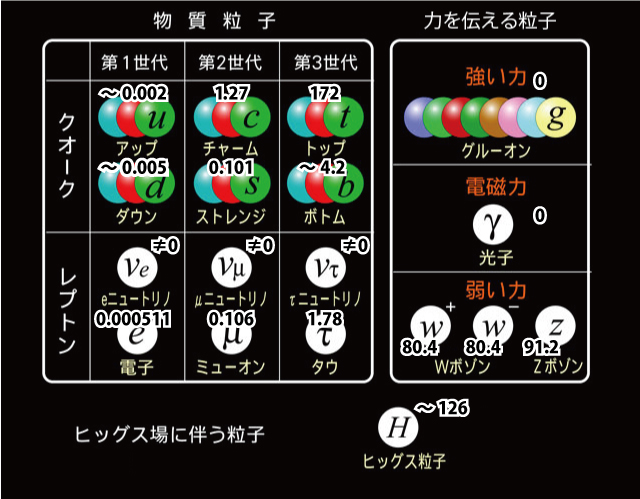
\includegraphics[width=250pt]{./Figure/Introduction/image_01.jpeg}
		\caption[標準模型]{標準模型~\cite{StandardModel}。各粒子の直上に示された数字は質量[GeV]を表す。}
		\label{StandardModel}
	\end{center}
\end{figure}

\section{Beyond the Standard Modelの探索}
標準理論はレプトンやクォークを始めとする素粒子の振る舞いを正確に記述するが、未だこの宇宙には多くの標準理論で説明できない謎が存在している。例として、暗黒物質(Dark Matter, DM)の正体は何か、超高エネルギースケールにおいて力は統一されるのか、ニュートリノの質量の起源とは何か、などが挙げられる。これらの謎に対して、TeVスケールを想定した理論がこれらの謎を解き明かすことが期待されている。一方で、現状のLarge Hadron Collider (LHC)における測定ではこれらの理論で存在が予言される新粒子は発見されていない。そのために、広い視野を持って新たな可能性を探ることが改めて重要となっている。LHCにおける発見が困難な原因として、新物理が重い、新物理で導入される新粒子が強い相互作用をしない、未発見の粒子が縮退した質量スペクトルである、などの要因が存在する可能性がある。もしくは、新粒子が軽いが相互作用の強さが小さいためコライダー実験では検証できない範囲にある可能性も挙げられる。

重心エネルギーが数百$\SI{}{GeV}$を超えるような加速器で粒子衝突を行い、$\SI{}{TeV}$スケール粒子の探索やそれに関連した結合定数などの測定を行う高エネルギー実験と、$\SI{}{GeV}$程度のエネルギーでより高い衝突頻度を持ち、相互作用の小さい$\SI{}{GeV}$スケールの新粒子を探索する固定標的実験は、BSMの広いパラメータスペースを探索する上で相補的に重要である。以下では、そのような新物理の一例を示す。

\subsection{Higgsボソンの精密測定}
2012年にLHCにおいてHiggsボソンが発見され、その存在が証明された。しかし依然としてその詳細な特性は明らかになっていない。例えば、HiggsセクターにおけるHiggsボソンの崩壊分岐比及び質量を極めて精密に測定することは新物理の証拠を見つける上で有力な手法となる。特に、崩壊分岐比を1\%以下の精度まで精密に測定することによりTeVスケールにおける新物理において生じる数\%のSMからのズレを発見することが多くの理論により提唱されている~\cite{Snowmass}。
Higgs質量や崩壊分岐比は表\ref{HiggsDecay}に示す多くの崩壊モードの観測を行うことにより測定される。

\begin{table}[h]
	\begin{center}
		\begin{tabular}{|ccc|}
		\hline
		崩壊モード&分岐比&$\sigma\times BR(\SI{}{fb})$\\\hline\hline
		$h\rightarrow b\bar{b}$&65.7\%&232.8\\\hline
		$h\rightarrow c\bar{c}$&3.6\%&12.7\\\hline
		$h\rightarrow gg$&5.5\%&19.5\\\hline
		$h\rightarrow WW^*$&15.0\%&53.1\\\hline
		$h\rightarrow \tau^+\tau^-$&8.0\%&28.2\\\hline
		$h\rightarrow ZZ^*$&1.7\%&6.1\\\hline
		$h\rightarrow \gamma\gamma$&0.29\%&1.02\\\hline		
		\end{tabular}
	\end{center}
	\caption[Higgsボソンの崩壊モード]{Higgsボソンの崩壊モード}
\label{HiggsDecay}
\end{table}


%%%%%%%%%%%%%%%%%%%%%%%%%%%%%%%%%%%%%%%%%%%%%%%%%%%%%%%%%%%%%%%%%%%%%%%%%%
\begin{comment}
これに加えて、Higgs-strahlung (図\ref{Higgs})により生成されるHiggsボソンの情報は崩壊分岐比を測定する上で重要な要素の一つである。この反応では、HiggsボソンはZボソンの反跳粒子として得られるので、Higgsボソンの崩壊モードによらずZボソンの崩壊にのみ着目することでヒッグス粒子の任意の粒子への崩壊断面積$\sigma_{ZH}\times BR\ (H\rightarrow X)\ (X = b, W, \tau, \ldots)$の測定を行うことができる。
\end{comment}
%%%%%%%%%%%%%%%%%%%%%%%%%%%%%%%%%%%%%%%%%%%%%%%%%%%%%%%%%%%%%%%%%%%%%%%%%%


\begin{figure}[h]
	\begin{center}
		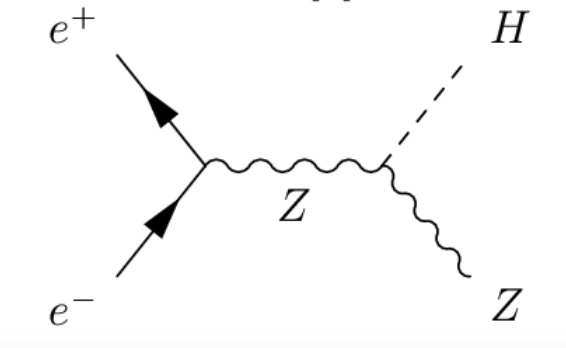
\includegraphics[width=150pt]{./Figure/Introduction/eeZZH.png}
		\caption[Higgs-strahlungのファインマンダイアグラム]{Higgs-strahlungのファインマンダイアグラム}
		\label{Higgs}
	\end{center}
\end{figure}

\subsection{超対称性}
超対称性は新物理探索の中で最も有望視され、これまでのコライダー実験でその理論に基づく新粒子の探索が行われてきた。SM粒子のパートナーとして、スピンが$1/2$だけ異なる超対称性パートナーを仮定し、RパリティやSMパートナーとの結合定数などのパラメータを考慮する。Rパリティは
\[
R\equiv(-1)^{3(B-L)+2S}
\]
によって定義される値で、超対称性粒子は$R=-1$、SM粒子は$R=1$をもつ。ここで、$S$はスピン、$B$はバリオン数、$L$はレプトン数である。

超対称性粒子の主な例を表\ref{SUSY_particle}に示す。%これらの他に、荷電Winoと荷電Higgsinoの混合状態である Chargino ($\chi^\pm$)やZino、Photinoと中性Higgsinoの混合状態であるNeutralinoが挙げられる。

\begin{table}[H]
	\begin{center}
		\begin{tabular}{|ccc|}
		\hline
		フェルミオン&超対称性パートナー&超対称性パートナーを示す記号\\\hline\hline
	        electron&selectron&$\tilde{e}$\\\hline
	        muon&smuon&$\tilde{\mu}$\\\hline
	        tauon&stauon&$\tilde{\tau}$\\\hline
	        electron neutrino&electron sneutrino&$\tilde{\nu_e}$\\\hline
	        muon neutrino&muon sneutrino&$\tilde{\nu_\mu}$\\\hline
	        tau neutrino&tau sneutrino&$\tilde{\nu_\tau}$\\\hline
	        up quark&scalar up quark&$\tilde{u}$\\\hline
	        down quark&scalar down quark&$\tilde{d}$\\\hline
	        charm quark&scalar charm quark&$\tilde{c}$\\\hline
	        strange quark&scalar strange quark&$\tilde{s}$\\\hline
	        top quark&scalar top quark&$\tilde{t}$\\\hline
	        bottom quark&scalar bottom quark&$\tilde{b}$\\\hline
	        \hline
	        ゲージボソン&超対称性パートナー&超対称性パートナーを示す記号\\\hline\hline
	        photon&photino&$\tilde{\gamma}^0$\\\hline
	        gluon&gluino&$\tilde{g}$\\\hline
	        W Boson&wino&$\tilde{W}^\pm$\\\hline
	        Z Boson&zino&$\tilde{Z}^0$\\\hline
	        %Higgs Boson&higgsino&$\tilde{H}^0,\tilde{H}^\pm$\\\hline
	        \hline
		\end{tabular}
	\end{center}
	\caption[超対称性パートナーの例]{超対称性パートナーの例。}
\label{SUSY_particle}
\end{table}

%%%%%%%%%%%%%%%%%%%%%%%%%%%%%%%%%%%%%%%%%%%%%%%%%%%%%%%%%%%%%%%%%%%%%%%%%%%%%%%%%%%
\begin{comment}
\begin{table}[H]
	\begin{center}
		\begin{tabular}{|ccc|}
		\hline
		フェルミオン&超対称性パートナー&超対称性パートナーを示す記号\\\hline\hline
	        電子(electron)&スカラー電子(selectron)&$\tilde{e}$\\\hline
	        ミューオン(muon)&スカラーミューオン(smuon)&$\tilde{\mu}$\\\hline
	        タウオン(tauon)&スカラータウオン(stauon)&$\tilde{\tau}$\\\hline
	        電子ニュートリノ(electron neutrino)&スカラー電子ニュートリノ(electron sneutrino)&$\tilde{\nu_e}$\\\hline
	        ミューニュートリノ(muon neutrino)&スカラーミューニュートリノ(muon sneutrino)&$\tilde{\nu_\mu}$\\\hline
	        タウニュートリノ(tau neutrino)&スカラータウニュートリノ(tau sneutrino)&$\tilde{\nu_\tau}$\\\hline
	        アップクォーク(up quark)&スアップスクォーク(scalar up quark)&$\tilde{u}$\\\hline
	        ダウンクォーク(down quark)&スダウンスクォーク(scalar down quark)&$\tilde{d}$\\\hline
	        チャームクォーク(charm quark)&スチャームスクォーク(scalar charm quark)&$\tilde{c}$\\\hline
	        ストレンジクォーク(strange quark)&スストレンジスクォーク(scalar strange quark)&$\tilde{s}$\\\hline
	        トップクォーク(top quark)&ストップスクォーク(stop squark)&$\tilde{t}$\\\hline
	        ボトムクォーク(bottom quark)&ボトムクォーク(s squark)&$\tilde{d}$\\\hline
	        \hline
	        ゲージボソン&超対称性パートナー&超対称性パートナーを示す記号\\\hline\hline
	        光子(photon)&ヴィーノ(Bino)&$\tilde{B_0}$\\\hline
	        グルーオン(gluon)&グルイーノ(gluino)&$\tilde{g}$\\\hline
	        Wボソン(W Boson)&ウィーノ(wino)&$\tilde{W}^\pm$\\\hline
	        Z ボソン(Z Boson)&グルイーノ(zino)&$\tilde{W}^0$\\\hline
	        Higgs ボソン(Higgs Boson)&ヒッグシーノ(higgsino) &$\tilde{H}$\\\hline
	        \hline
		\end{tabular}
	\end{center}
	\caption[超対称性パートナーの例]{超対称性パートナーの例。}
\label{SUSY_particle}
\end{table}

\end{comment}
%%%%%%%%%%%%%%%%%%%%%%%%%%%%%%%%%%%%%%%%%%%%%%%%%%%%%%%%%%%%%%%%%%%%%%%%%%%%%%%%%%%%%%

さらに、GauginoおよびHiggsinoが混合して生じるcharginoやneutralinoの存在も予測されている。

超対称性粒子はその質量の順序に関して幾つかの仮説があるが、最も軽い超対称性粒子(the Lightest SUSY Particle、 LSP)としては通常Nuetralinoが考えられる。Neutralinoの混合として、Wino-likeもしくはHiggsino-likeとして存在している場合、LSPと質量差がほとんど無いBosinoが存在することが示唆されている。一方、Bino-likeなNeutralinoがLSPである場合、LSPと次に軽い超対称性粒子との間に大きな質量差が生じる。しかし、この場合、初期宇宙のLSP生成および消滅の間にバランスが必要になるため、DMの存在が予期される。SUSY粒子の消滅を高めるための方法として$\tilde{\tau}$の対消滅を通じて生成するものがある。

SUSYは$\ \SI{}{GeV} - \ \SI{}{TeV}$まで探索が行われているが、未だ発見されておらず質量や結合定数に対する制限が与えられている。そのため、現在さらに高エネルギー領域へと探索範囲が広げられつつある。

加速器でSUSYを探索する上で、コライダー実験で SUSY を探索する上で、R パリティが保存するモデルを考えると、最終状態に必ず偶数個のLSPが現れる。
SUSY粒子のカスケード崩壊\footnote{粒子が物質中に入射すると連続的に相互作用を引き起こす。これをカスケード崩壊と呼ぶ。第2章で詳しく述べる。}で現れるSM粒子の信号と、LSPによるエネルギー・運動量欠損からSUSY探索を行う。

\subsection{Axion/ALPs}
BSMでその存在が予想されている粒子の一つに擬スカラー粒子が挙げられる。この粒子は物理学における強いCP問題の解を探索する上で提案された~\cite{Axion}~\cite{Axion1}。  quantum chromodynamics (QCD)におけるLagrangianは
%\begin{equation}
\[
{\cal L}_{QCD} = \sum_{q} \bar{q}(i \cancel D - m_q e^{i\theta_q \gamma_5})q -\frac{1}{4} G^{a \mu\nu}G^a_{\mu\nu} + \theta \frac{g_s^2}{32\pi^2}G^{a\mu\nu}\tilde{G}^a_{\mu\nu}
%\end{equation}
\]
と記される。ここで、$\theta_q$および$\theta$はそれぞれクォーク質量の位相およびゲージ変換における定数である。これらの定数はPおよびT変換に対して保存しないので、一般にはQCDにおけるCP対称性の破れが生じると考えられていた。しかし、中性子の電気双極子モーメント$d_n$の測定から得られる$\theta_q + \theta$の値はこの予測値よりも小さく、従ってCP破れの程度が小さくなることが示されている。これを強いCP問題と呼ぶ。

この問題の解の一つとして与えられたのが擬スカラー粒子のQCD axionである。もしこの粒子が存在すると仮定すれば、QCDラグランジアンは
\begin{equation}
{\cal L} = \left(\frac{a}{f_a} - \bar{\theta}\right) \frac{\alpha_s}{8\pi }G^{\mu\nu a}\tilde{G}^a_{\mu\nu} 
\end{equation}

\[
a : \textrm{QCD axion}
\]
\[
\bar{\theta} = \theta_q + \theta
\]
となり、$\bar{\theta}$の項が相殺されるため、CP保存が成立する。Axionの質量の候補としては$\SI{}{\mu eV}$ 程度の極めて小さいものから TeV スケール以上の大きいものまで幅広く、もし十分に小さいのであれば、高エネルギー加速器を使用することなく、小規模の実験でも発見されうる。Axionを探索するための実験は今日まで行われてきているが、未だ発見されていない。

Axionと同様に自発的対称性の破れから生じる擬南部ゴールドストーン粒子をAxion Like Particles (ALPs)と呼び、これらの粒子もまた探索の対象となっている。ALPsは多くの理論により予言されており、その質量や結合の強さは様々に及んでいる。一つのモデルとして、次の有効ラグランジアンによって記述されるALPが提案されている。
\begin{equation}
\delta{\cal L} =-\frac{1}{4}g_{a\gamma\gamma}aF_{\mu\nu}\tilde{F}^{\mu\nu}+\frac{1}{2}(\partial_{\mu}a)^2-\frac{1}{2}m_a^2a^2
\end{equation}

ここで$a$はALPを指しており、$F$はフォトン場の強さ、$\tilde{F}^{\mu\nu}=\epsilon_{\mu\nu}\lambda_\rho F^{\lambda\rho}/2$である。
このALPの角度に対する生成微分断面積は
\begin{equation}
\frac{d\sigma_{\gamma a}}{d\theta_a} \cong \frac{\alpha g^2_{a\gamma\gamma}k^4\theta_a^3}{t4^2} G_2(t)
\end{equation}
で表される。ここで、$G_2(t)\cong Z^2(a'^2t/(1+a7^2t))^2/(1+t/d)^2$、$Z$は標的の原子番号、$a'=112Z^{-1/3}/m_e$、$d=\SI{0.164}{GeV^2}$、$m_e=\SI{511}{keV}$は電子質量である。
一方、崩壊幅は
\begin{equation}
\Gamma_a = \frac{g_{a\gamma\gamma^2 m_a^3}}{64\pi}
\end{equation}
であり、2光子へと崩壊する。電子ビームのビームダンプへの照射からALPが生成されるファインマンダイアグラムを図\ref{ALP_int}に示す。aがALPを示しており、その崩壊で生じる2光子対をカロリメータによって検出する。

\begin{figure}[h]
	\begin{center}
		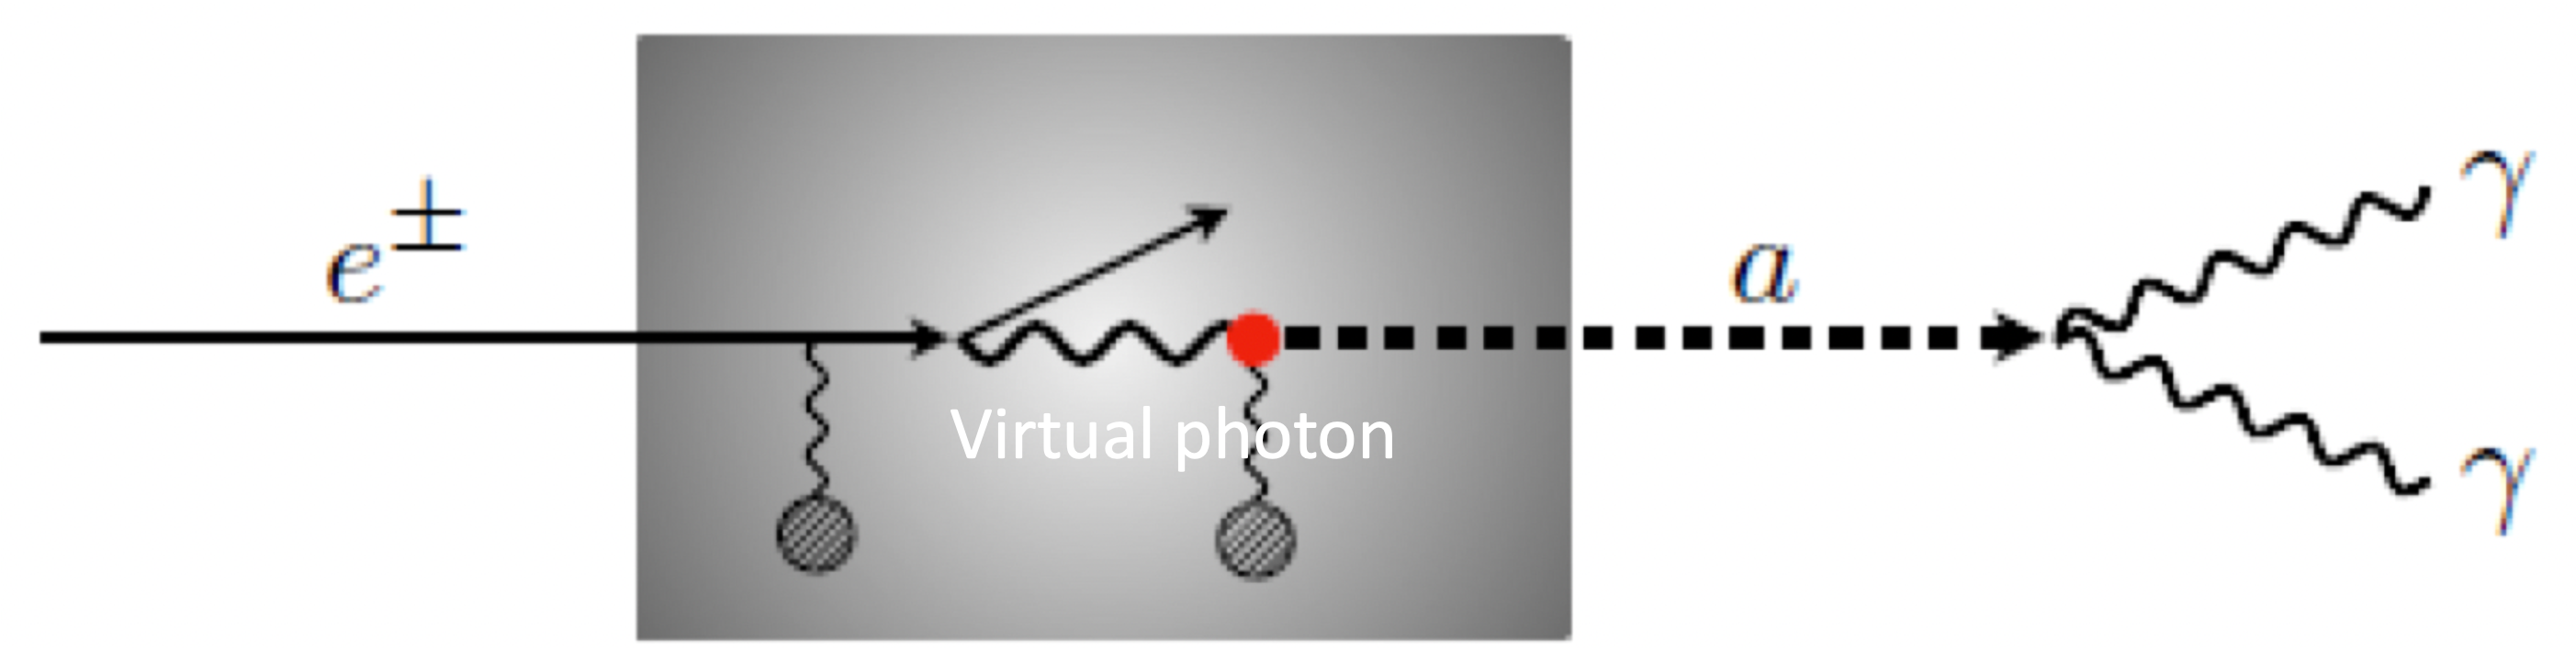
\includegraphics[width=350pt]{./Figure/Introduction/ALP_int.png}
		\caption[ビームダンプによるALPの生成を示すファインマンダイアグラム]{電子ビームのビームダンプによるALPの生成を示すダイアグラム。aがALPを示している。}
		\label{ALP_int}
	\end{center}
\end{figure}


%この粒子は強いCP問題のPeccei-Quinn解の候補として得られ、QCD Axionと名付けられた。Axionは初期宇宙において冷たいDMとして残存しうることが宇宙論の観測から推測され、現在のダークマター候補の一つとして有力視されている。

%これらの事実から、LHCで見つかりにくい新物理に感度がある$e^+e^-$ Higgs Factoryと結合が小さい新物理を探せる固定標的実験の両面で新物理を探索する必要がある。

%今回の研究では$e^+e^-$ Higgs factoryと$e^+e^-$固定標的実験の双方で、共通の技術を使うことができるカロリメーター技術に着目し、その実装と各実験での応用を検討した。
%例えば、ダークマターが挙げられる。この物質はエネルギー密度に関して宇宙の構成要素の25\%を占めると推定され、このダークセクターに属する粒子は標準理論のSM粒子と非常に弱く相互作用するため、検出が難しいと考えられている\cite{Axion}。現在までに数々のSMを超える理論(Beyond Standard Model、 BSM)が発表され、この粒子の特性を予想している。

\section{新物理探索におけるカロリメータの役割}
新物理イベントが生じていれば、特定のイベントに対して実験で測定される散乱断面積に標準理論で記述される散乱断面積とのズレが生じ、そのズレを精度よく測定することによって新物理が存在することがより強く示唆される。新物理探索を行う上でのカロリメータの役割はビームの衝突によって生じたジェットや中性粒子を特定し、そのエネルギーを測定することである。
%%%%%%%%%%%%%%%%%%%%%%%%%%%%%%%%%%%%%%%%%%%%%%%%%%%%%%%%%%%%%%%%
\begin{comment}
カロリメータで測定されたジェットエネルギーは解析を通じて再構成され、不変質量へと変換される。不変質量$m_0$は光速$c$、粒子のエネルギーを$E$、粒子の運動量を$\mathbf{p}$とすると、以下の式で表される。
\begin{equation}
(m_0c^2)^2 =E^2-c^2|\mathbf{p}|^2
\end{equation}

%モンテカルロ(MC)シミュレーションはハードウェアでは観測できないバックグラウンド事象を推定するために有効であり、新物理探索を行う上では必要不可欠である。
%シミュレーションを元にした不変質量分布により、バックグラウンド事象とシグナル事象が区別され、もしここで新物理が観測できていれば、SMに基づいたシミュレーションでは存在しないスペクトラムが現れている。
\end{comment}
%%%%%%%%%%%%%%%%%%%%%%%%%%%%%%%%%%%%%%%%%%%%%%%%%%%%%%%%%%%%%%%
新物理探索を行う上で必要となるのがジェットエネルギー分解能の向上である。
%再構成される不変質量スペクトラムには事象由来の自然幅に加えて、統計量の平方根に依存する統計誤差と測定器に依存する系統誤差が生じる。この影響により断面積の小さい反応はもし観測できていたとしてもピークが埋没してしまい存在を確認することが難しくなる。
例として、ILC計画においてW - Zボソンの不変質量を3$\sigma$の精度で識別するためには角度の不確定性を無視すると少なくとも3-4\%のジェットエネルギー分解能を必要とする~\cite{PFATest}。
この精度はハードウェアの改善だけでなく、ソフトウェアによる解析アルゴリズムの改善が必要不可欠である。

%新物理が観測された証明をより確固たるものとするためにはルミノシティを高め、統計誤差を減らすだけでなく、検出器や検出アルゴリズムに依存した系統誤差を低減させることが重要となる。
%その上で課題となるのが、粒子の識別精度やバックグラウンドとの分離などである。相互作用によって生じた粒子が崩壊して検出器に入射した時、そのタネとなる粒子の種類が異なっていても、検出器により取得された情報だけでは同定が困難なケースが存在する。

\begin{comment}
\begin{itemize}
\item PFAを用いてジェットエネルギー分解能の向上させることによりTPCにおいて荷電粒子のエネルギーをより精度良く測定する
\item Ecalにおいて入射する光子のエネルギーをより精度良く測定する
\end{itemize}
の2つが挙げられる。
\end{comment}

\section{ILC計画}
国際リニアコライダー計画(International Linear Collider、 ILC)はHiggsボソンの詳細な特性を解明し、新物理探求を行うことを主目的とした次世代の電子陽電子直線加速器計画である。その概形は図\ref{ILCaccelerator}に示されている。建設予定地は東北地方の北上山地であり、安定した地盤とトンネル掘削のしやすさを特徴としている。ILCはその名の通り世界中の研究者が共同で実験計画および実行を行う国際プロジェクトとして進行しており、世界各地の研究機関で加速器や各検出器などの開発が行われている。

\begin{figure}[h]
	\begin{center}
		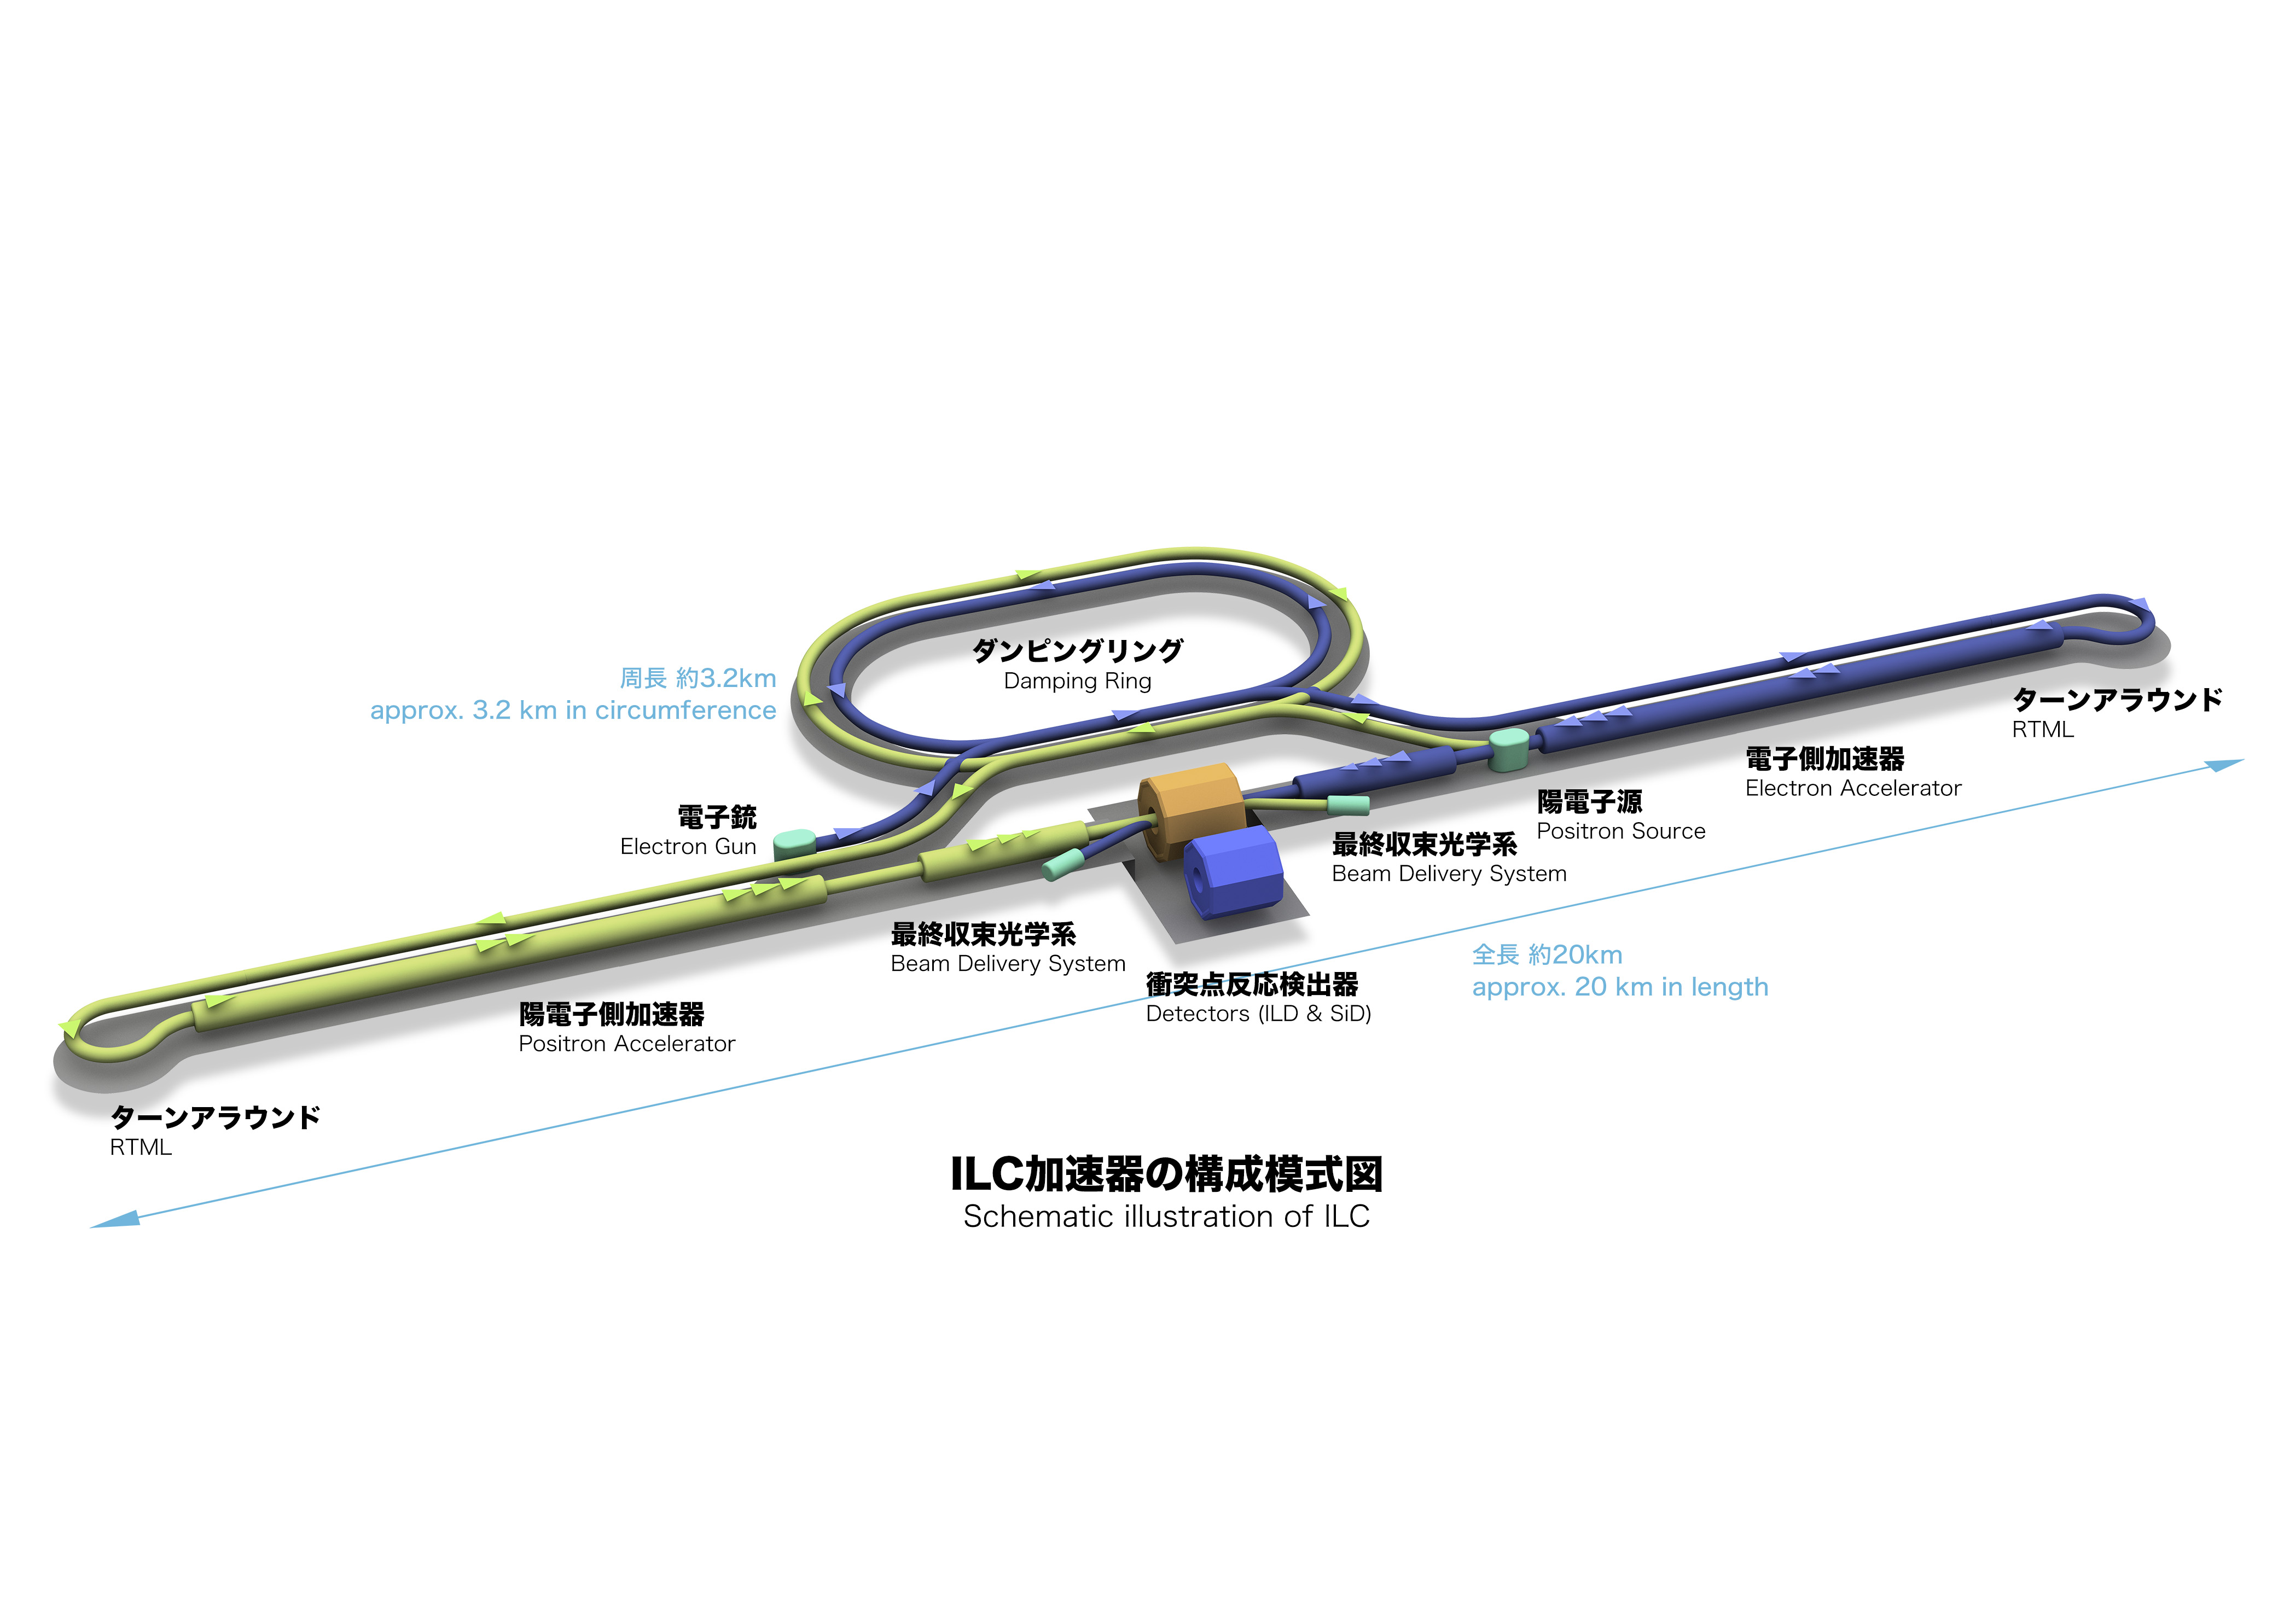
\includegraphics[width=350pt]{./Figure/Introduction/image_02.jpg}
		\caption[ILC加速器]{ILC加速器~\cite{StandardModel}。}
		\label{ILCaccelerator}
	\end{center}
\end{figure}


ILCは電子陽電子直線加速器を有するという特徴から、同じ高エネルギー実験である陽子陽子円形加速器Large Hadron Collider (LHC)にない長所を持ち、異なる役割を果たす。

ILCの運転開始時はHiggsボソン生成を起こすために最適のエネルギーである$\SI{250}{GeV}$の重心系エネルギーで陽電子と電子を衝突させる。これはHiggsボソンの質量がおよそ$\SI{125}{GeV}$であることに由来する。直線型加速器は円形加速器と異なり、加速器直線部分の延長、もしくは加速技術の向上によって$\SI{1}{TeV}$以上のエネルギーまで拡張可能である。

さらに、円形加速器では重心系エネルギーの増加に伴って制動放射によるエネルギーロスの増大が発生し大きな課題となるが、線形加速器ではその影響が無く、十分に高いエネルギーまでエネルギーロスを少なく加速を行うことを可能とする。

また、LHCでは陽子が強い相互作用に伴う反応を引き起こすために非常に多くのバックグラウンドの影響を受けるが、ILCは素粒子である陽電子と電子のコライダーであるためにその影響が相対的に少なくて済むため、精密測定や稀な崩壊を観測することに長所を持つ。

一方で、円形コライダーは繰り返し周回して粒子衝突を行うことが可能であるが、ILCは直線加速器のため粒子の衝突は1回のみである。そのため、ルミノシティを上げてイベントの生成回数を高める必要があり、電子および陽電子のビームは十分にエミッタンスを絞って衝突が引き起こされる。ルミノシティとは、ビーム衝突型加速器におけるビーム衝突回数を示した値で、単位時間当たりの反応数を$N$、断面積を$\sigma$とすると、単位時間当たりのルミノシティ$L$は、
\begin{equation}
L = \frac{N}{\sigma}
\end{equation}
で表される。

ILCの加速器には高純度ニオブを用いた超伝導加速空洞が使用される。超伝導は極低温において電流の流れる際の抵抗値が極めて0に近くなる現象である。これにより、加速空洞中の表面において消費されるエネルギーを低減させることができる。この影響を低減することは、超伝導を実現するための冷却に必要となる電力を差し引いても大きなメリットである。加速空洞は図\ref{cavity}に示すように9つのセルが接合された構造を持ち、内部で電場を構成することにより粒子ビームを加速させる。さらに、超伝導現象を引き起こすために液体ヘリウムによって極低温に保たれている。

\begin{figure}[h]
	\begin{center}
		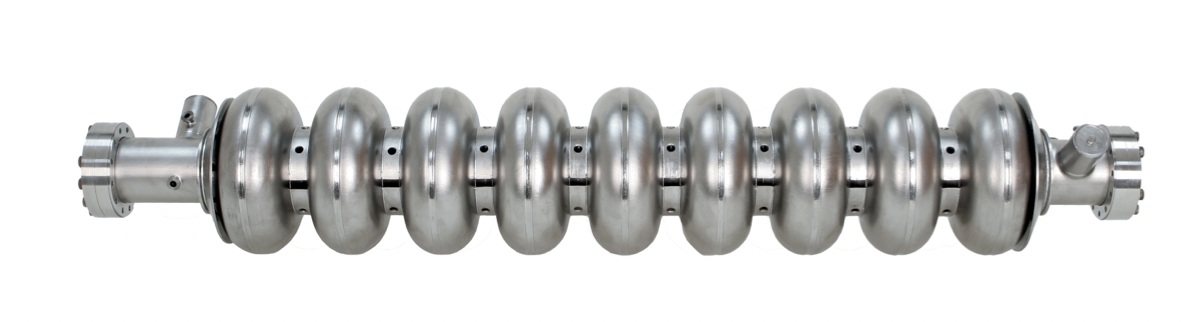
\includegraphics[width=250pt]{./Figure/Introduction/cavity.png}
		\caption[ILC超伝導加速空洞]{ILC超伝導加速空洞}
		\label{cavity}
	\end{center}
\end{figure}


\begin{comment}
\section{ILCの物理}
ILCの運転開始エネルギーである$\SI{250}{GeV}$では、先ほど述べたようにHiggsボソン生成過程であるZh随伴過程が主要な寄与を示す。この散乱断面積を図\ref{ZhCrossSection}に示す。エネルギーの増加とともに徐々にWW fusionの断面積も増大し、エネルギーアップデート後の実験ではこの寄与も重要となる。Zh随伴生成の有益な点としては、ZボソンがHiggsボソンの反跳として生じるため、Higgsボソンの直接観測をすることなくその分岐比や質量を測定することが可能な点である。

\begin{figure}[h]
	\begin{center}
		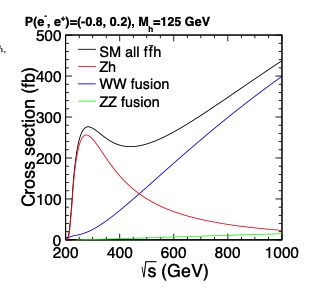
\includegraphics[width=250pt]{./Figure/Introduction/image_03.jpg}
		\caption[重心系エネルギー$\SI{250}{GeV}$付近の主要過程の断面積]{重心系エネルギー$\SI{250}{GeV}$付近の主要過程の断面積}
		\label{ZhCrossSection}
	\end{center}
\end{figure}

Zh随伴過程などのプロセスにより生成されたHiggsボソンはさまざまな崩壊モードを持ち、その一覧が表\ref{HiggsDecay}に示されている~\cite{ILCPhysics}。

\begin{table}[h]
	\begin{center}
		\begin{tabular}{|c|c|c|}
		\hline
		崩壊モード&分岐比&$\sigma\cdot BR(\SI{}{fb})$\\\hline\hline
		$h\rightarrow b\bar{b}$&65.7\%&232.8\\\hline
		$h\rightarrow c\bar{c}$&3.6\%&12.7\\\hline
		$h\rightarrow gg$&5.5\%&19.5\\\hline
		$h\rightarrow WW^*$&15.0\%&53.1\\\hline
		$h\rightarrow \tau^+\tau^-$&8.0\%&28.2\\\hline
		$h\rightarrow ZZ^*$&1.7\%&6.1\\\hline
		$h\rightarrow \gamma\gamma$&0.29\%&1.02\\\hline		
		\end{tabular}
	\end{center}
	\caption[Higgsボソンの崩壊モード]{Higgsボソンの崩壊モード。}
\label{HiggsDecay}
\end{table}

Higgsボソンに関する重要な測定として、質量および生成断面積、崩壊分岐比がある。これらのパラメータを精密に測定することは、LHCで観測された$\SI{125}{GeV}$の共鳴が標準理論にあるHiggsボソンと一致するのか、それとも別の構造を持った粒子なのかという重要な問いに答えるために必要となる。

\begin{figure}[h]
	\begin{center}
		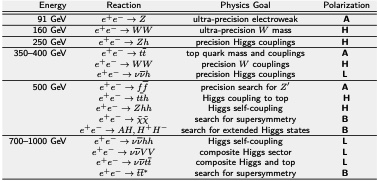
\includegraphics[width=370pt]{./Figure/Introduction/image_04.jpg}
		\caption[各重心系エネルギーで主要となる過程]{各重心系エネルギーで主要となる過程}
		\label{DominantProcess}
	\end{center}
\end{figure}

\begin{table}[h]
	\begin{center}
		\begin{tabular}{cccc}
		\hline
		エネルギー&過程&物理目標\\\hline
		$\SI{91}{GeV}$&$e^+e^-\rightarrow Z$&電弱精密測定\\
		$\SI{160}{GeV}$&$e^+e^-\rightarrow WW$&W質量精密測定\\
		$\SI{250}{GeV}$&$e^+e^-\rightarrow Zh$&Higgs結合精密測定\\
		$350 - \SI{450}{GeV}$& $e^+e^-\rightarrow t \bar{t}$&tクォークの質量および結合定数精密測定\\
		\end{tabular}
	\end{center}
	\caption[各重心系エネルギーで主要となる過程の表]{各重心系エネルギーで主要となる過程の表}
\label{DominantProcess_table}
\end{table}
\end{comment}


\section{ILC検出器}
ILC加速器の衝突点にはILD (International Large Detector)とSiD (Silicon Detector)の2種類の検出器が置かれることが計画されている。それぞれの検出器に含まれる構成はほぼ同じだが、一つの違いとしてILDは飛跡検出器にTPCとシリコン検出器を用いている一方で、SiDは飛跡検出器全体がシリコン検出器であることが挙げられる。ILDとSiDのそれぞれの検出器が独立に測定を行い、実験の信頼性の向上を図っている。本研究はこのうち、ILDを対象としている。
加速器実験に使用される大型の検出器は、一つの装置で非常に多くの種類データを測定するためにさまざまなモジュールを搭載した複合検出器として設計される。ILDに含まれる主な構成要素が表\ref{Detector}に挙げられている。

飛跡検出はVTX、SITおよびTPCで測定されたデータを基に解析が行われる。ILC計画においてはbクォークとcクォークの測定が非常に重要となり、高精度のフレーバーの特定が要求される。この解析をflavor taggingと呼ぶ。これらのクォークは相対論的効果を無視するとかなり短い距離($b$クォークは$400-\SI{500}{\mu m}$、$c$クォークは$20-\SI{300}{\mu m}$)しか走らないという特性から、飛跡検出器はビーム相互作用点からおよそ$\SI{1.6}{cm}$の非常に近い位置に置かれ、$\SI{3}{\mu m}$以下の高精度の位置分解能を持つように設計されている。

ECALおよびHCALからなるカロリメータでは光子および電子、中性ハドロンのエネルギー測定を行う。カロリメータについては第2章で詳しく述べるが、大きな特徴としてそれぞれのレイヤーを非常に微細化しており、高い位置分解能での測定を可能としている。

検出器だけでは入射してくる荷電粒子の運動量を求めることはできないため、ソレノイドを用いて入射粒子の軌道を曲げることが必要となる。ILDでは$\SI{3.5}{T}$超伝導ソレノイドを利用する。このソレノイドによって生じた磁場は入射粒子の運動量に応じて曲率半径が変化し、この半径を測定することで運動量を求めることが可能となる。また、Iron Yokeはミューオンとそれ以外の粒子を識別するために磁場によって生じたflux returnの影響からソレノイドの磁束が拡散するのを防ぐことを主目的とする。
%また、電源装置などによって生じる外部磁場が問題となるため、Iron Yokeを配置してそれらの影響を低減させる。
%その他にも、入射した粒子の運動量を知るために磁場によって曲げられた曲率を測定するための$\SI{3.5}{T}$超伝導ソレノイドや、外部から侵入してくる磁場の影響を低減させるためのIron Yokeが備えられる。

%ビームモニターには、表\ref{BeamMonitor}に示される検出器群が用いられる。ビームには高いルミノシティが要求されるため、加速器稼働中はその状態が一定となっていることを確認することが重要である。


\begin{table}[h]
	\begin{center}
		\begin{tabular}{c|c|c}
		\hline
		検出器名&検出器略称&役割\\\hline\hline
		Vertex Detector&VTX&崩壊点検出\\
		Silicon Internal Tracker&SIT&崩壊点付近の飛跡検出\\
		Time Projection Chamber&TPC&飛跡検出\\
		Electromagnetic Calorimeter& ECAL&電子および光子のジェットエネルギー測定\\
		Hadron Calorimeter&HCAL&中性ハドロンのジェットエネルギー測定\\\hline
		\end{tabular}
	\end{center}
	\caption[ILDに導入される検出器モジュール]{ILCに導入される検出器モジュール}
\label{Detector}
\end{table}

\begin{comment}
\begin{table}[h]
	\begin{center}
		\begin{tabular}{cccc}
		\hline
		検出器名&検出器略称&役割\\\hline
		VTX&Vertex Detector&崩壊点検出\\
		Silicon Internal Tracker&SIT&崩壊点付近の飛跡検出\\
		Time Projection Chamber&TPC&飛跡検出\\
		Electromagnetic Calorimeter& ECAL&電子および光子のジェットエネルギー測定\\
		\end{tabular}
	\end{center}
	\caption[ILC加速器に備えられるビームモニター]{ILC加速器に備えられるビームモニター}
\label{BeamMonitor}
\end{table}
\end{comment}



\section{EBES実験}
Electron Beam dump Experiment at Switchyard 3 (EBES)実験は茨城県・高エネルギー加速器研究所にあるSuper KEKB Linacを用いてALPsを探索することを目的とした実験である。実験はSuper KEK  LinacのSwitching yard 3 (SY3)で行われる。この実験では、電子・陽電子ビームをビームダンプへと入射させ、内部で仮想光子が生じた後、ALPsへと崩壊するイベントを観測する。ALPsはビームダンプを通過して光子ペアへと崩壊するため、直接観測が可能となる。Linac は$\SI{4}{GeV}$までの陽電子ビームと$\SI{7}{GeV}$までの電子ビームが利用可能である。

実験により排除される領域に関して、他の実験と比較したのが図\ref{ALP_world}である~\cite{EBES}。

\begin{figure}[h]
	\begin{center}
		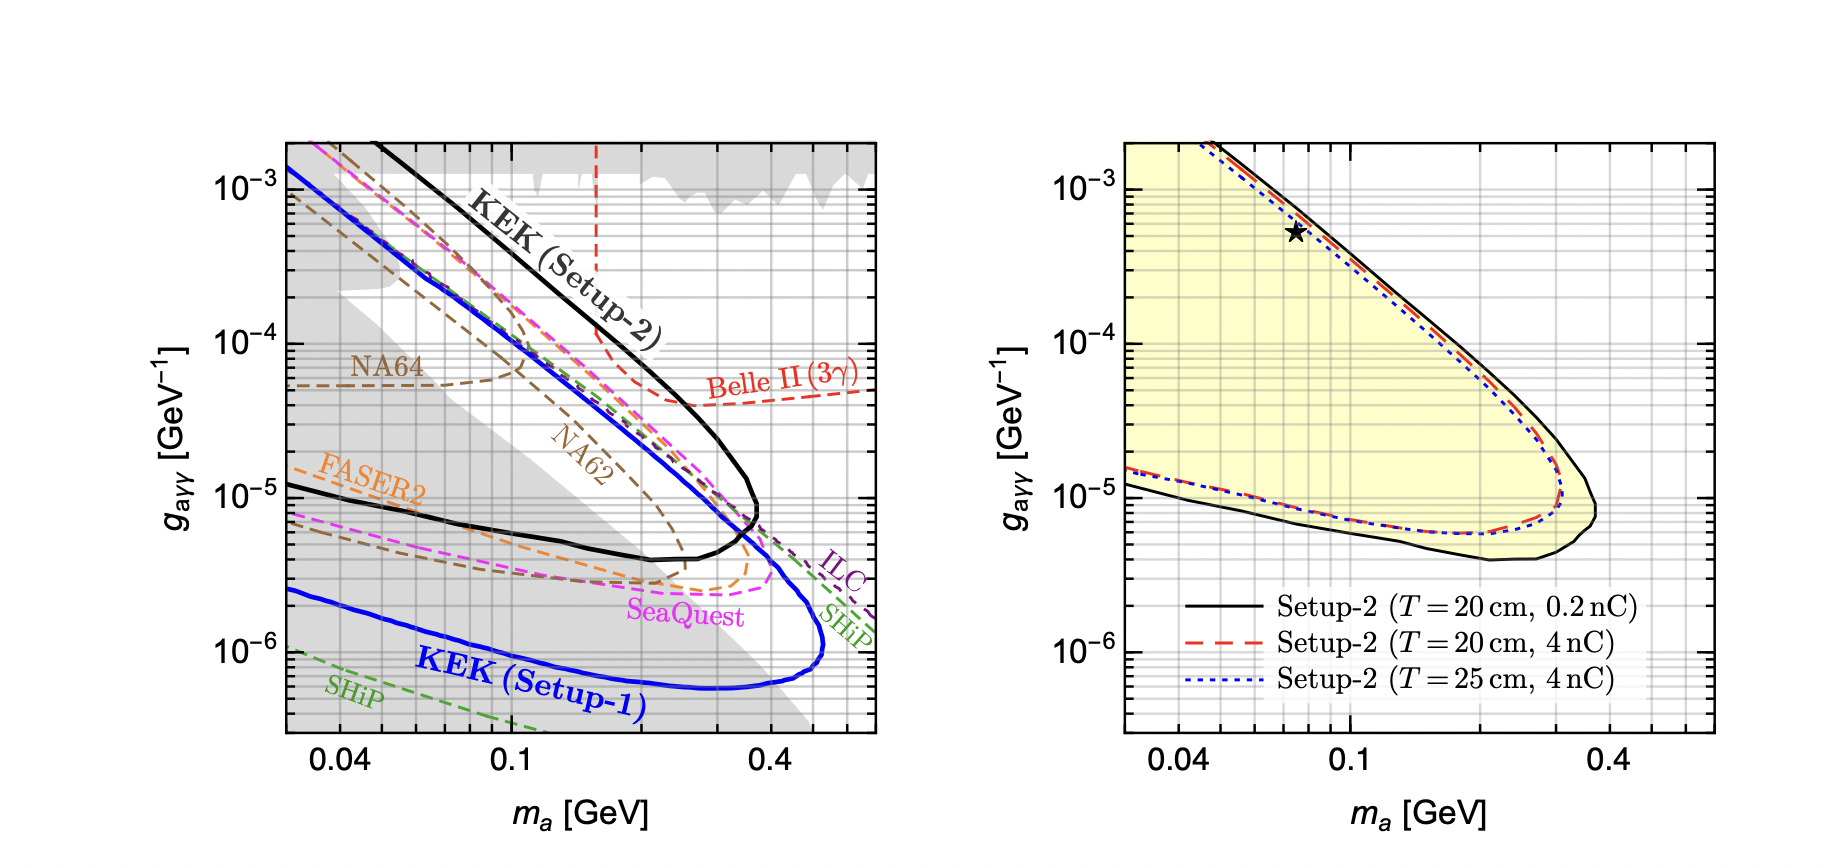
\includegraphics[width=370pt]{./Figure/Introduction/ALP_world.png}
		\caption[EBES実験によるALPの95\%C.L.]{EBES実験によるALPの95\%C.L.。ALPsの結合定数および質量について示されている。左図は他の実験との比較で、右図は第5章で説明するSetup-2の変更による差を表している。}
		\label{ALP_world}
	\end{center}
\end{figure}

SHiPやFASER2などの実験と比較すると、より短寿命のALPsをより低コストで探索することが本実験の特徴の一つである。

\section{本研究の目的}
%ILC計画・EBES計画の双方に関して、相互作用において生じる荷電粒子および光子のエネルギーを正確に測定することは測定精度を高めるために必要である。%本研究ではそれぞれの実験に対してハードウェア・ソフトウェア双方の面から個別に研究を行った。
%EBES実験の目的であるALPs探索は
本研究では、将来の電子陽電子実験に向けたカロリメトリー技術の開発を目的とする。新物理探索を目的とした実験として、ILC実験はPFAによってジェットエネルギー分解能よく測定を行い、ヒッグス精密測定を向上させるためにカロリメトリーは重要な技術である。また、EBES実験によるALPs探索は未知の新物理の手がかりとなりうる興味深い実験であり、発見を確固たるものとするためには優れた性能を持つカロリメトリー技術が必要である。そこで、ILCカロリメータプロトタイプに使用される技術に着目した。ILCのカロリメータの特徴として非常に微細化されていることを挙げたが、2光子を分離し質量を再構成するためにはこの微細化による高い位置分解能が効果的である。%また、ジェットエネルギー分解能を高めるために使用されるPFAに関しても、EBES実験において系統誤差を低減させ稀なALPs崩壊反応を検出するために有用である。
EBES実験には主に全吸収のカロリメータを利用することが予定されているが、この特徴からILCのカロリメータを一部利用することで2光子の分離とバックグラウンドの除去性能の向上を行う案が検討されている。
今回はその性能をさらに高めることを目的として深層学習技術を用いたカロリメータクラスタリングの開発を行い、シミュレーションデータによる評価を行った。同時に、EBES実験で使用されるカロリメータである鉛ガラス検出器に対してもエネルギー較正やエネルギー分解能測定を行った。今回開発したカロリメータ技術はILCの将来のビームダンプ実験にも活用でき、より高いエネルギーのALP探索を行うことも可能である。


\section{本論文の流れ}
2章・3章はILCカロリメーターおよび深層学習に関する導入となる。2章では、カロリメトリー技術の詳細を述べる。3章では、本研究で使用した深層学習技術について概要を説明する。
4章では、深層学習技術を利用したカロリメトリーアルゴリズムの改善について述べる。
5章はKEKで行われたEBES実験のバックグラウンド測定実験について概観する。
6章では検出器のエネルギー較正実験についてその概要と解析結果について説明する。
7章は本論文のまとめであり、今後の展望についても考察を与える。

 % !TEX root = ../MasterThesis.tex

\chapter{カロリメトリー技術} \label{sec:DeepLearning}
本章では、ILC実験およびEBES実験のために用いられるカロリメトリー技術について述べる。2.1節ではカロリメトリーの基本的な動作原理となる物理現象について説明する。2.2節ではカロリメータを用いた測定技術について述べる。2.3節ではカロリメータにおいてジェットエネルギー分解能向上のためのアルゴリズムの一つであるParticle Flow Algorithm (PFA)について説明する。
\section{カロリメトリーに関する物理現象}
素粒子実験で検出対象となる粒子は、検出器との相互作用を生じさせることにより、その位置やエネルギーなどの情報を測定することが可能となる。これまでに行われてきた理論計算や実験などによって、粒子の検出器に対する応答が明らかとなっている。
\subsection{荷電粒子と物質の相互作用}
荷電粒子は物質中では原子内に存在する原子核や電子と電磁相互作用を行う。主には励起や電離といった反応が起こり、入射してきた荷電粒子は徐々に速度を落としていく。Bethe-Blochの行った計算によると、荷電粒子が物質中で落とす単位長あたりのエネルギー損失は
\begin{equation}
-\frac{dE}{dx} = \frac{4\pi \alpha^2 \hbar^2 q^2 n_e}{m_e\beta^2}\left[\ln\left(\frac{2m_ec^2 \beta^2\gamma^2}{I}\right)-\beta^2-\frac{\delta(\gamma)}{2}\right]
\end{equation}

\begin{table}[H]
	\begin{center}
		\begin{tabular}{ll}
			$\alpha$ : 微細構造定数($\simeq 1/137$) & $\hbar$ : ディラック定数\\
			$n_e$ = $\rho N_A Z/A$ : 電子密度& $q$ : 入射粒子の持つ電荷 \\
			$N_A$ : アボガドロ数 & $\beta = v / c$ ($v$ : 入射粒子の速度、$c$ : 光速) \\
			$Z$ : 吸収体の原子番号 & $\gamma$ = $(1-\beta^2)^{-1/2}$ \\
			$A$ : 吸収体の質量数 & $I$ : イオン化ポテンシャル \\
			\multicolumn{2}{l}{$\delta$ : 吸収体原子内の電子による電場の遮蔽効果のパラメータ} \\
		\end{tabular}
	\end{center}
\end{table}

となる。このBethe-Blochの式に基づく入射粒子のエネルギーに対するエネルギー損失の大きさを示したグラフを図\ref{Bethe}に示す\cite{PDG_Interaction}。
\begin{figure}[H]
	\begin{center}
		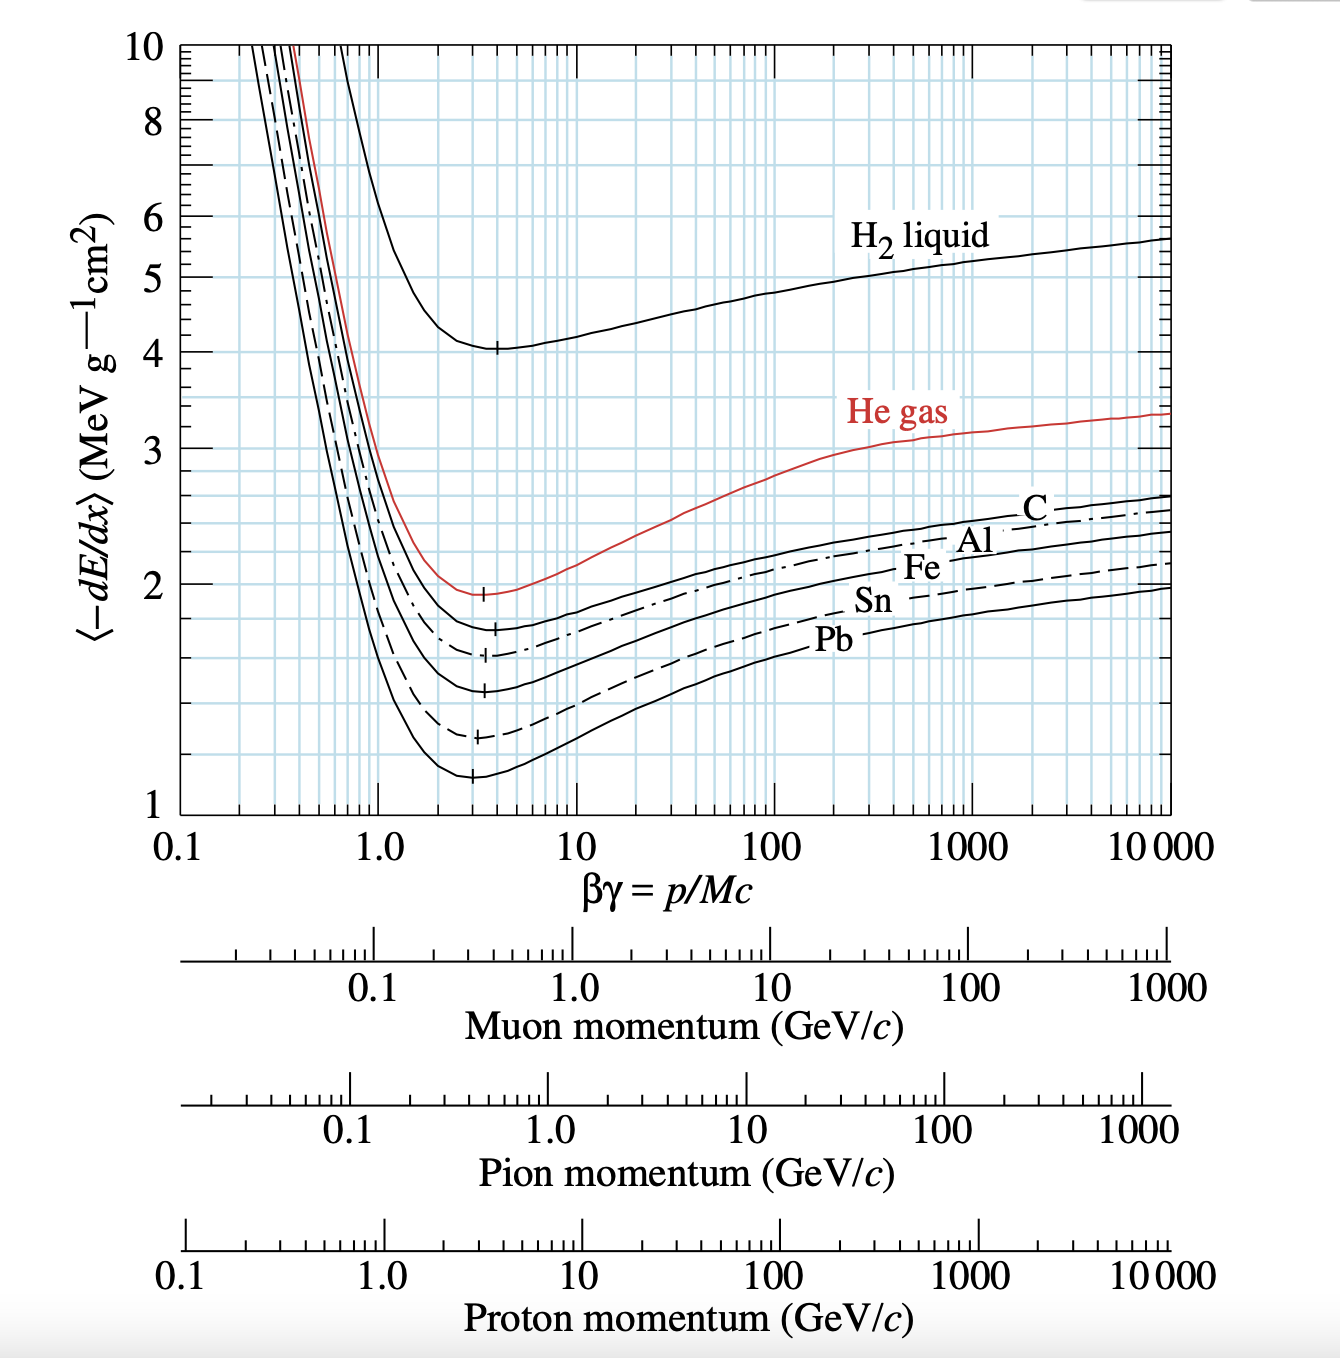
\includegraphics[width=370pt]{./Figure/EcalDetector/Bethe.png}
		\caption[Bethe-Blochの式に基づくエネルギー損失]{Bethe-Blochの式に基づくエネルギー損失}
		\label{Bethe}
	\end{center}
\end{figure}


この図から分かるように、エネルギー損失は特定の運動量において最小となり、それより高い運動量ではゆるやかに上昇する。エネルギー損失が最小となる運動量付近にある粒子をMIP (Minimum Ionizing Particle)と呼ぶ。

\subsection{光子と物質の相互作用}
光子は電荷を持たないため、荷電粒子とは異なる相互作用を引き起こす。主として生じる相互作用は、光電効果、コンプトン散乱、電子対生成の3つである。

\begin{description}
\item 光電効果:

エネルギーの小さい光子が物質中に入射すると、原子内の電子が光子のエネルギーを全て吸収し、吸収したエネルギーが束縛エネルギー以上であればその電子は物質外へと放出される。この現象を光電効果と呼ぶ。相対論的速度に近づくほど光子の十分にエネルギーが大きいとき、その断面積は
\begin{equation}
\Phi_{\mathrm{photo}} = 4\alpha^4 \sqrt{2} Z^5 \phi_0 \left(\frac{m_ec^2}{h\nu}\right)^{\frac{7}{2}}
\end{equation}
と表される\cite{HEPDetector}。ただし、$m_e$は電子質量、$\phi_0 = \frac{8\pi r_e^2}{3}=6.651\times 10^{-25}\SI{}{cm^2}$($r_e$は古典電子半径)は古典的なトムソン散乱の断面積である。
	
	
\item コンプトン散乱:

光子のエネルギーがある程度大きくなると、電子が光電効果による全てのエネルギーを吸収しきれなくなり、電子と光子の散乱現象が生じる。これがコンプトン散乱である。コンプトン散乱の断面積は次のクライン-仁科の公式
\begin{equation}
\frac{d\sigma_{\mathrm{compton}}}{d\Omega}=\frac{r_e^2}{2}\frac{1}{[1+\gamma(1-\cos\theta)]^2}\left(1+\cos^2\theta+\frac{\gamma^2(1-\cos\theta)^2}{1+\gamma(1-\cos\theta)}\right)
\end{equation}
により記述されることが知られている。

\item 電子対生成:

光子のエネルギーがおよそ$\SI{1.02}{MeV}$以上になると、光子が物質中の原子核と相互作用することにより生じる電子対生成現象が起こり始める。これは光子のエネルギーが電子および陽電子の質量へと転換されることにより電子陽電子ペアが生じる現象である。カロリメータ中における高エネルギー反応においてはこの電子対生成反応が主要な寄与を示し、後述する電磁シャワーを発生させる一因となる。この断面積は近似的に
\begin{equation}
\sigma_{\mathrm{pair}} \approx \frac{7}{9}\frac{A}{N_AX_0}
\end{equation}
で表される。ただし、$A$は物質の質量数、$N_A$はアボガドロ数、$X_0$は放射長である。ここで、放射長$X_0$は
\begin{equation}
X_0= 4\left(\frac{\hbar}{mc}\right)^2Z(Z+1)\alpha^3n_a\ln\left(\frac{183}{Z^{1/3}}\right)
\end{equation}
と表され、この長さは荷電粒子のエネルギーが$1/e$に減少するまでに物質中を通過する平均距離を示している。

\end{description}
	
これらの3つの現象の断面積は、光子のエネルギーおよび媒質によって大きな違いが生じる。炭素および鉛に対して、照射した光子のエネルギーごとに各反応の断面積を示したものを図\ref{photonInteract}に示す。

\begin{figure}[H]
	\begin{center}
		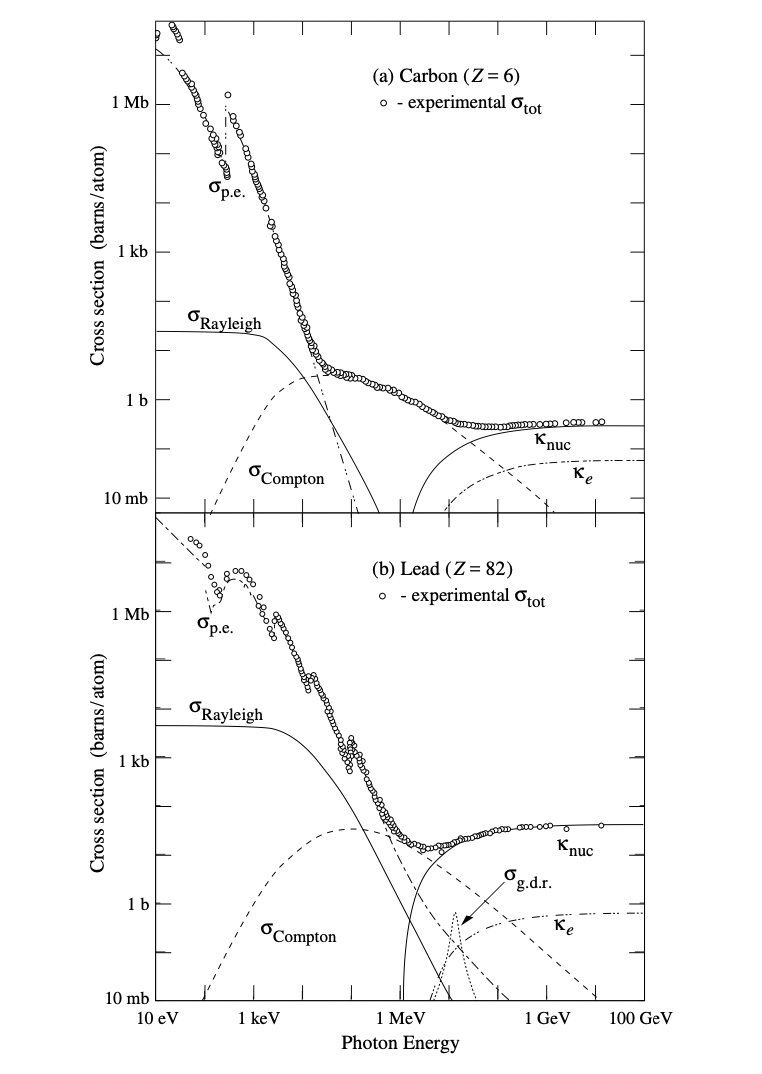
\includegraphics[width=370pt]{./Figure/EcalDetector/PhotonInteract.png}
		\caption[光子のエネルギーに対する相互作用断面積]{炭素C、鉛Pbに入射した時の光子のエネルギーに対する相互作用断面積\cite{PDG_Interaction}。}
		\label{photonInteract}
	\end{center}
\end{figure}


\subsection{制動放射}
荷電粒子は前述の通りイオン化や光電効果などによってエネルギーを失う他、制動放射(bremsstrahlung)と呼ばれる、主に原子核との相互作用によって光子が放出される現象とともに大きなエネルギー損失が生じる。この反応は電子や陽電子に対して主要なエネルギー損失となりうる。

この反応による平均のエネルギー損失は
\begin{equation}
-\frac{dE}{dx} = \frac{E}{X_0}
\end{equation}
と表される。

制動放射によって失われる放射長あたりのエネルギー損失と電子のエネルギーが等しくなる時のエネルギーを臨界エネルギー(Critical Energy)と呼ぶ。この時のエネルギー損失はエネルギーを$E$とすると、
\begin{equation}
\left|\frac{dE}{dx}\right|_{\mathrm{brems}}\approx  \frac{E}{X_0}
\end{equation}
となる。

\subsection{チェレンコフ光}
荷電粒子が物質中を通過するとき、同じ媒質中を通過する光よりも速く運動する場合、チェレンコフ光と呼ばれる光が発生する。
この速度$v_{\mathrm{particle}}$は光速$c$、粒子の速度を$\beta c$、生じたチェレンコフ光の数を$n$とすると、
\begin{equation}
\beta c = v_{\mathrm{particle}} > c/n
\end{equation}
で与えられ、生じるチェレンコフ光により生じる円錐の開き角$\theta_C$は
\begin{equation}
\cos\theta_C=\frac{1}{\beta n(\omega)}
\end{equation}


この時放出される光子の数はチェレンコフ光の波長$\lambda$および単位長さ$x$あたり、

\begin{equation}
\frac{d^2 N}{d\lambda dx}=\frac{2\pi z^2\alpha}{\lambda^2}\left(1-\frac{1}{\beta^2n^2(\lambda)}\right)
\end{equation}

と表される。ただし、荷電粒子の電荷$z$、微細構造定数を$\alpha$、$n(\omega)=1/(\beta \cos\theta_C)$である。
チェレンコフ光の数は粒子の数および飛程にほぼ比例している。

%%%%%%%%%%%%%%%%%%%%%%%%%%%%%%%%%%%%%%%%%%%%%%%%%%%%%%%%%%%%%%%%
\begin{comment}
このチェレンコフ光により荷電粒子が失うエネルギーは、荷電粒子の電荷を$z$、微細構造定数を$\alpha$、光速$c$、粒子の速度を$\beta c$、チェレンコフ光の波長を$\omega$として、
\begin{equation}
-\frac{dE}{dx} = z^2 \frac{\alpha \hbar}{c} \int\omega d\omega\left(\1-\frac{1}{\beta^2n^2(\omega)}\right)
\end{equation}
と表される。
\end{comment}
%%%%%%%%%%%%%%%%%%%%%%%%%%%%%%%%%%%%%%%%%%%%%%%%%%%%%%%%%%%%%%%%

\subsection{電磁シャワーおよびハドロンシャワー}
十分に大きなエネルギーを持った荷電粒子および中性粒子が物質中に入射すると、電磁シャワーやハドロンシャワーのような特徴的な現象が生じる。

電磁シャワーは上で述べた電子対生成が関与している。光子が大きなエネルギーを持っている場合、その光子が変換されて生じた電子および陽電子もまた大きな運動エネルギーを持って放出される。この場合、電子が制動放射を起こすことにより新たな光子を生成することになる。この結果、エネルギーが十分小さくなるまで電子陽電子対生成と制動放射が繰り返し引き起こされる。

シャワーの大きさは、物質の厚さと放射長に依存する。シャワー内に含まれる合計の粒子数(光子や電子、陽電子)$N$は物質の厚さが放射長の$t$倍であるとすると、
\[
N = 2^t
\]
と表される。

%%%%%%%%%%%%%%%%%%%%%%%%%%%%%%%%%%%%%%%%%%%%%%%%%%%%%%
\begin{comment}
この時、生じるカスケードの最大厚み$t_{max}$は入射光子のエネルギーを$E_0$、臨界エネルギー$E_c$に対して、
\[
E(t_{\mathrm{max}}) = \frac{E_0}{2^{t_{\mathrm{max}}}}=E_c
\]
より、
\[
t_{\mathrm{max}} = \frac{\ln{\frac{E_0}{E_C}}}{\ln{2}}
\]
となる。
\end{comment}
%%%%%%%%%%%%%%%%%%%%%%%%%%%%%%%%%%%%%%%%%%%%%%%%%%%%%%


電磁シャワーの90\%のエネルギー損失が収まるように円筒領域を考えたときに、その円筒の半径をMoliere 半径と呼ぶ。Moliere 半径$R_M$は臨界エネルギーを$E_C$、放射長を$X_0$とすると、
\begin{equation}
R_M = X_0 \frac{21\ [\SI{}{MeV}]}{E_C}
\end{equation}
と表される。シャワーの全エネルギーのうち、$3.5R_M$には99\%のエネルギーが吸収されている。

ハドロンシャワーは荷電ハドロンおよび中性ハドロンが物質中に入射することで生じる。ハドロンシャワーは非常に複雑な過程が混在する。入射してきた高エネルギーハドロンは物質中の原子核および電子と非弾性散乱を行い、二次的な相対論的エネルギーハドロンの生成や$\SI{100}{MeV}$程度の核破砕核の放出、ハドロンによる原子核の破壊などが生じる。これらの核反応の連鎖によりシャワーを発生する。
一方、これらの相互作用の生成物に含まれる$\pi_0$中間子の発生は$\pi_0$から崩壊した$\gamma$線による電磁気的相互作用の寄与を伴う。この電磁シャワーはハドロンシャワーと比較して同じエネルギー損失あたりの発生粒子数が異なるので、大きな誤差要因となりうる。この影響を低減させるためにCompensationやDual-readoutといった検出器技術が開発されている。Compensationでは、電磁シャワーもハドロンシャワーもエネルギーあたり同じ信号強度になるようにしたり、検出器ハードウェアを工夫したりすることによって電磁成分とハドロン成分の差を小さくする技術である。その技術の一つであるDual-readout技術は荷電ハドロンおよび電磁シャワーをシンチレーション光とチェレンコフ光による2重読み出しによって測定を行い、それぞれの寄与を別々に測定するために開発されている。



\section{カロリメータ技術}
カロリメータは入射してきた光子や荷電粒子などによって生成されたシャワーをカロリメータ内で吸収することにより入射粒子のエネルギーを測定する。
この項では、カロリメータ検出器による粒子検出の原理について、説明を行う。2.2.1節および2.2.1節では全吸収カロリメータとそのうちの一種である鉛ガラス検出器について述べる。2.2.3節ではもう一つのカロリメータであるサンプリング型カロリメータについて取り上げる。

\subsection{全吸収型カロリメータ}
全吸収型カロリメータは検出器全体が吸収体となっており、電子や光子の入射で発生する電磁シャワーによるシンチレーション光やチェレンコフ光\cite{PDG_Cal}を検出し、光電子増倍菅(Photomultiplier Tube, PMT)により増幅する。これらの検出器には主に原子番号の大きな鉛ガラスやクリスタルが用いられ、一例として$\textrm{BaF}_2$やCsI(Tl)、LYSOなどが用いられる。これらの検出器はエネルギー分解能が高く、特に低エネルギーの粒子を精度良く測定するのに向いているが、これらの物質は微細分割のコストが高く、またエネルギー較正が難しい点が短所として挙げられる。

\subsection{鉛ガラス検出器}
鉛ガラスチェレンコフ検出器は入射した荷電粒子や光子の検出およびそのエネルギー測定を行うための検出器である。鉛ガラス中で電磁シャワーから放出される電磁シャワーに含まれる電子の一部は媒質中での光速を超え、チェレンコフ光を発生させる。%鉛ガラス検出器の表面を反射材に覆うことで、チェレンコフ光は内部で反射し検出器の一面に取り付けられたPMTへと集光される。
チェレンコフ光は空気と鉛ガラスの境界での全反射に加えて、表面を反射材で覆うことで内部で反射し、検出器の一面に取り付けられたPMTへと集光される。
発生するチェレンコフ光の光子数は入射した荷電粒子の数および飛程にほとんど比例し、電磁シャワーではエネルギーと粒子数が概ね比例するため、結果としてPMTにおいて光から変換された電気信号を測定することで荷電粒子のエネルギーを決定することが可能である。PMTは外部からの光に敏感であり、光の漏れがあると信号が大きくなるため、遮光を十分に行う必要がある。

今回EBES実験のために使用する鉛ガラス検出器はTRISTAN/TOPAZ実験で使用された、ビーム軸に対する面積が$150\times\SI{150}{mm^2}$、奥行きが$\SI{30}{cm}$の検出器である\cite{LeadGlass}。概形を図\ref{PbO}に示す。放射長に対する奥行きは$17.7X_0$に対応しており、検出器を構成する成分は55\%がPbO、45\%が$\textrm{SiO}_2$となっている。この検出器に対して光電子増倍菅を接続し、光検出を行う。

\begin{figure}[H]
	\begin{center}
		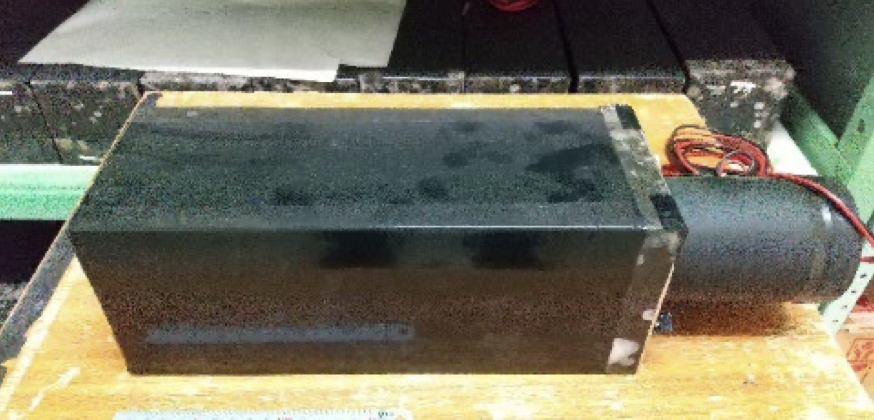
\includegraphics[width=370pt]{./Figure/EcalDetector/PbO.png}
		\caption[EBES実験に使用する鉛ガラス検出器]{EBES実験に使用する鉛ガラス検出器。}
		\label{PbO}
	\end{center}
\end{figure}


\subsection{サンプリング型カロリメータ}
サンプリング型カロリメータは吸収体と検出層を別々に構成することによって、微細化したカロリメータを構成することができる。光子や電子が入射すると、吸収体によって電磁シャワーへと変換され、シャワーによって運搬されたエネルギーが検出層において検出される。カロリメータに入射してきた粒子の全エネルギーに対する検出層の吸収エネルギーはサンプリング率と呼ばれ、サンプリング型カロリメータの性能を示す指標の一つとなっている。検出層には主に半導体やシンチレーター、ガスイオン検出器が用いられる一方、吸収層にはタングステンや鉛、鉄などといった原子番号の大きな金属が用いられる。サンプリング型カロリメータの構造については複数のタイプが考えられ、吸収層と検出層のプレートを交互に重ねたサンドイッチ構造のものやファイバーのような検出層を吸収体の中に埋め込むものなどがある。吸収層の間に挿入された検出層の多くのチャンネルから信号を読み出す方法が問題となり得るが、一つの解決策として読み出し回路を検出器内に挟み込んで読み出しを行なっている。

\subsection{SiW電磁カロリメータ}
ILDに使用される電磁カロリメータの一つとして、SiW電磁カロリメータ(SiW ECAL)が開発されている。その全体像を図\ref{SiW Ecal}に示す。このカロリメータはシリコン検出層とタングステン吸収層を交互に30層組み合わせたサンドイッチ構造を持つサンプリングカロリメータである。この節でそれぞれの特徴について述べた後、2.2.3節でシリコン検出層から送信されてきた信号を統括する読み出し回路について説明する。

\begin{figure}[H]
	\begin{center}
		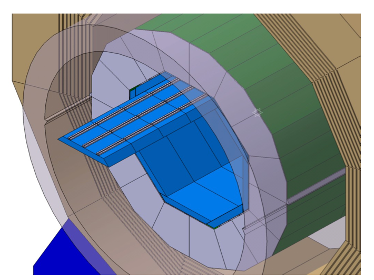
\includegraphics[width=250pt]{./Figure/EcalDetector/ILD_det_3D.png}
		\caption[ILD・ECALの全体像]{ILD ECALの全体像。青色で示されているのがECAL、緑色で示されているのがHCALである。}
		\label{SiW Ecal}
	\end{center}
\end{figure}


\begin{itemize}
\item シリコン検出層

ILDにおける電磁カロリメータは後に説明するParticle Flow Algorithm(PFA)を実行するために十分に微細化されている必要がある。そのためシリコン検出層は$1.0\times10^{8}$チャンネルまで微細化された検出器として開発が進められている。SiWECALを図\ref{ECAL_layer}に示す。それぞれの層にはFEVボードと呼ばれる電子回路が搭載されており、1枚のFEVボードには4枚のシリコンパッドが使用されている。

\begin{figure}[H]
	\begin{center}
		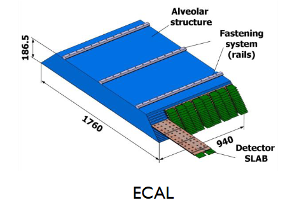
\includegraphics[width=250pt]{./Figure/EcalDetector/ECAL_layer.png}
		\caption[SiWECAL]{SiWECALの模式図。図中にはFEVボードが示されている。}
		\label{ECAL_layer}
	\end{center}
\end{figure}

シリコンは半導体の一種であり、荷電粒子検出器の原料として用いることができる。ここではそのうち、PN接合型と呼ばれる検出器の動作原理について述べる。半導体には多く存在しているキャリア電荷が正か負かによってP型およびN型の2種類に分けることができ、PN接合型の検出器はこの2種類の半導体素子を組み合わせることによって製造される。二つの半導体素子の中間には、正キャリア(正孔)と負キャリア(電子)が結合することにより空乏層と呼ばれる電気的に中性の領域が生じる。この空乏層に荷電粒子が入射すると、光電効果やコンプトン散乱により電子がP型半導体側へと放出される。一方、もともと電子が存在していた部分は負電荷欠乏となるため、電気的に正のキャリアが存在していると考えられ、この正キャリアはN型半導体へと移動する。この電子および正孔のペアを電子正孔対と呼ぶ。以上の電子正孔対の移動により、シリコン検出器内に電流が流れ、この電流を検出することによりガンマ線の測定を行うことが可能となる。一方、荷電粒子の場合は空乏層に入射するとイオン化が生じることにより電子の移動が起こり、以下ガンマ線の場合と同様にして荷電粒子の検出を行う。また、シリコン素子の両側に外部から電圧を印加すると検出領域である空乏層が広がるため、有感領域を拡大することができる。電圧を上げるほど空乏層の厚みは増加し、素子全体が空乏層となることを完全空乏化と呼ぶ。


現在のプロトタイプでは、1枚のパッドは大きさが$180\times \SI{180}{mm^2}$、厚さが$320-\SI{650}{\mu m}$となっている。シリコンパッドを4枚組み合わせることでActive Signal Units (ASU)が構成され、それぞれのシリコンパッドは大きさが$90\times \SI{90}{mm^2}$となっている。1枚のシリコンパッドにはさらに256個のチャンネルがあり、1チャンネルのピクセルサイズは$5.5\times\SI{5.5}{mm^2}$である。1枚のFEVボードを図\ref{FEV}に示す。

\begin{figure}[b]
	\begin{center}
		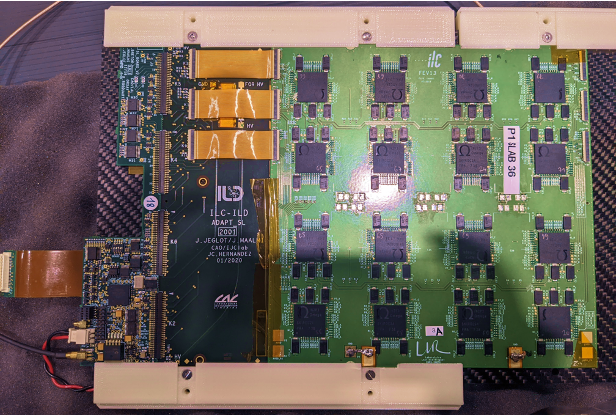
\includegraphics[width=250pt]{./Figure/EcalDetector/ECAL_board.png}
		\caption[FEVボード]{FEVボードの写真。16枚のASICチップとSLボードが搭載されている。}
		\label{FEV}
	\end{center}
\end{figure}

それぞれのASUには読み出しのためのSKIROC2 (A)と呼ばれるApplication Specific Integrated Circuits (ASICs)が備え付けられている。

\item タングステン吸収層

それぞれのシリコン検出層の間にはタングステン吸収層が挿入されており、カロリメータ全体で30枚となる。一枚の厚さは$\SI{2.1}{mm}$もしくは$\SI{4.2}{mm}$であり、厚さの合計は$24X_0$となる。タングステンを吸収層に選んだ理由としては、相互作用長が放射長のおよそ28倍となるため光子とハドロンの識別が優れている点や、$R_M$が小さくなる点が挙げられる。
\end{itemize}


%\subsection{シリコン検出器の動作原理}
%シリコンは半導体の一種であり、ガンマ線および荷電粒子検出器の原料として用いることができる。ここではそのうち、PN接合型と呼ばれる検出器の動作原理について述べる。半導体には多く存在しているキャリア電荷が正か負かによってP型およびN型の2種類に分けることができ、PN接合型の検出器はこの2種類の半導体素子を組み合わせることによって製造される。二つの半導体素子の中間には、正キャリアと負キャリアが結合することにより空亡層と呼ばれる電気的に中性の領域が生じる。この空乏層にガンマ線が入射すると、光電効果やコンプトン散乱により電子がP型半導体側へと放出される。一方、もともと電子が存在していた部分は負電荷欠乏となるため、電気的に正のキャリア(正孔)が存在していると考えられ、この正キャリアはN型半導体へと移動する。この電子および正孔のペアを電子正孔対と呼ぶ。以上の電子正孔対の移動により、シリコン検出器内に電流が流れ、この電流を検出することによりガンマ線の測定を行うことが可能となる。一方、荷電粒子の場合は空乏層に入射するとイオン化が生じることにより電子の移動が起こり、以下ガンマ線の場合と同様にして荷電粒子の検出を行う。特にシリコン素子の両側に外部から電圧を印加すると検出領域である空乏層が広がるため、有感領域を拡大することができる。電圧を上げるほど空乏層の厚みは増加し、素子全体が空乏層となることを完全空乏化と呼ぶ。

%\subsection{シンチレーション光}

\section{カロリメトリーにおけるPFAの利用}
ジェットエネルギー分解能を向上させるための技術として、PFAと呼ばれる手法があり、ILC実験ではこの手法を採用することで精度良くジェットエネルギー測定を行う。2.3.1節ではPFAの概要を説明する。2.3.2節ではPFAがどのようにILCのソフトウェアに組み込まれているかを説明するために、ILCにおけるソフトウェアエコシステムの全体像について述べる。2.3.3ではILCにおけるPFAアルゴリズムとして利用されているPandoraPFAについてその概要を述べる。2.3.4ではPandoraPFAを利用した際の粒子識別性能およびジェットエネルギー分解能を確認する。

\subsection{PFA}
電子陽電子ビームの衝突によって高エネルギーのクォークペアが生じると、クォークは単独では存在できないため強い相互作用による破砕化(フラグメンテーション)によって2つのジェットと呼ばれる粒子朿が形成される。これらのジェットは複数の荷電ハドロンや中性ハドロンを伴って飛跡検出器を通過した後、カロリメータへと入射する。

PFAは光子、荷電粒子、中性ハドロンのそれぞれを別々の検出器によって検出することによりジェットエネルギー分解能を向上させるための手法である。PFAを使う測定器では、光子は電磁カロリメータ、荷電粒子は飛跡検出器、中性ハドロンはハドロンカロリメータで検出が行われる。それぞれのジェットが持つエネルギーの全エネルギーに対する割合は荷電粒子がおよそ60\%、光子がおよそ30\%、中性ハドロンがおよそ10\%となる。荷電粒子(ほとんどがハドロンである)をハドロンカロリメータではなく飛跡検出器で測ることで、ジェットエネルギー分解能が大幅に向上する。ILC検出器における各粒子の分離の様子を図\ref{PFA_ILC}に示す。検出器は内側から、飛跡検出器、ECAL、HCALを示している。
\begin{figure}[H]
	\begin{center}
		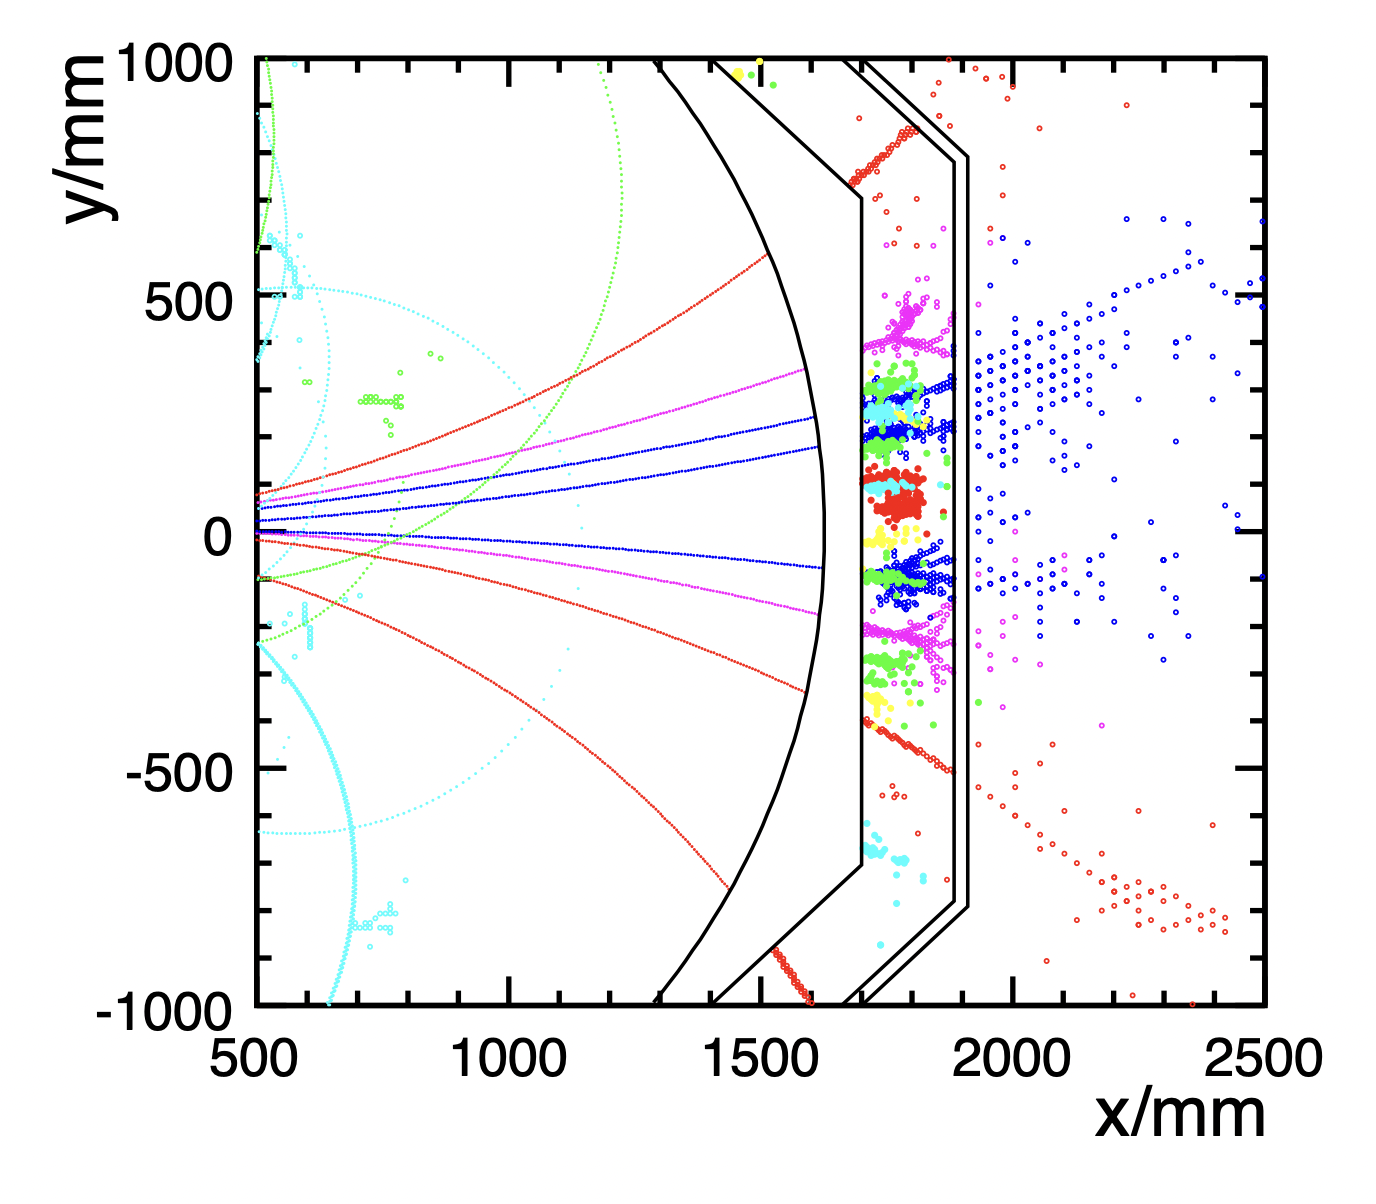
\includegraphics[width=370pt]{./Figure/EcalDetector/PFA_ILC.png}
		\caption[ILCにおける粒子識別の様子]{ILCにおける粒子識別の様子。異なる種類の粒子が異なる色によって識別されている。}
		\label{PFA_ILC}
	\end{center}
\end{figure}



各粒子を分離するために、検出器は非常に微細化されている必要がある。そのため、ILDに備えられる検出器は非常に多くのチャンネルを持った検出器となっている。

\begin{comment}
\subsection{iLCSoft}
ILCは現在計画段階にあり、検出器のジオメトリの設計や、目的とする新物理探索などについて決定するためにはソフトウェア技術が欠かせない。iLCSoftは線形加速器におけるシミュレーションや飛跡再構成、物理解析を行うためのソフトウェアエコシステムであり、LCIOやMarlin、DD4hepといったフレームワークを含んでいる。

iLCSoftを含むILC Softwareのワークフローを図\ref{iLCSoft_workflow}\cite{ILCSoftware}に示す。

まず、whizardやphyssimなどを用いて、目的とするイベントの生成が行われる。生成されたイベントはstdhepやlcioと呼ばれるフォーマットで保存される。これらのイベントを入力として、iLCSoftは検出器シミュレーションやイベント再構成を行う。検出器シミュレーションはGeant4をベースにしたDD4Simによって、またイベント再構成はMarlin(Modular Analysis \& Reconstruction for the LINear collider)と呼ばれるアプリケーションによって実行される。Marlinの中に含まれるのがジェットエネルギー再構成のためのPandoraPFAや飛跡再構成のためのTracking、崩壊点検出のためのLCFIPlusなどである。これらの情報がDSTMergedによって統合され、最終的にRootやPythonなどによる解析が行われる。

\begin{figure}[H]
	\begin{center}
		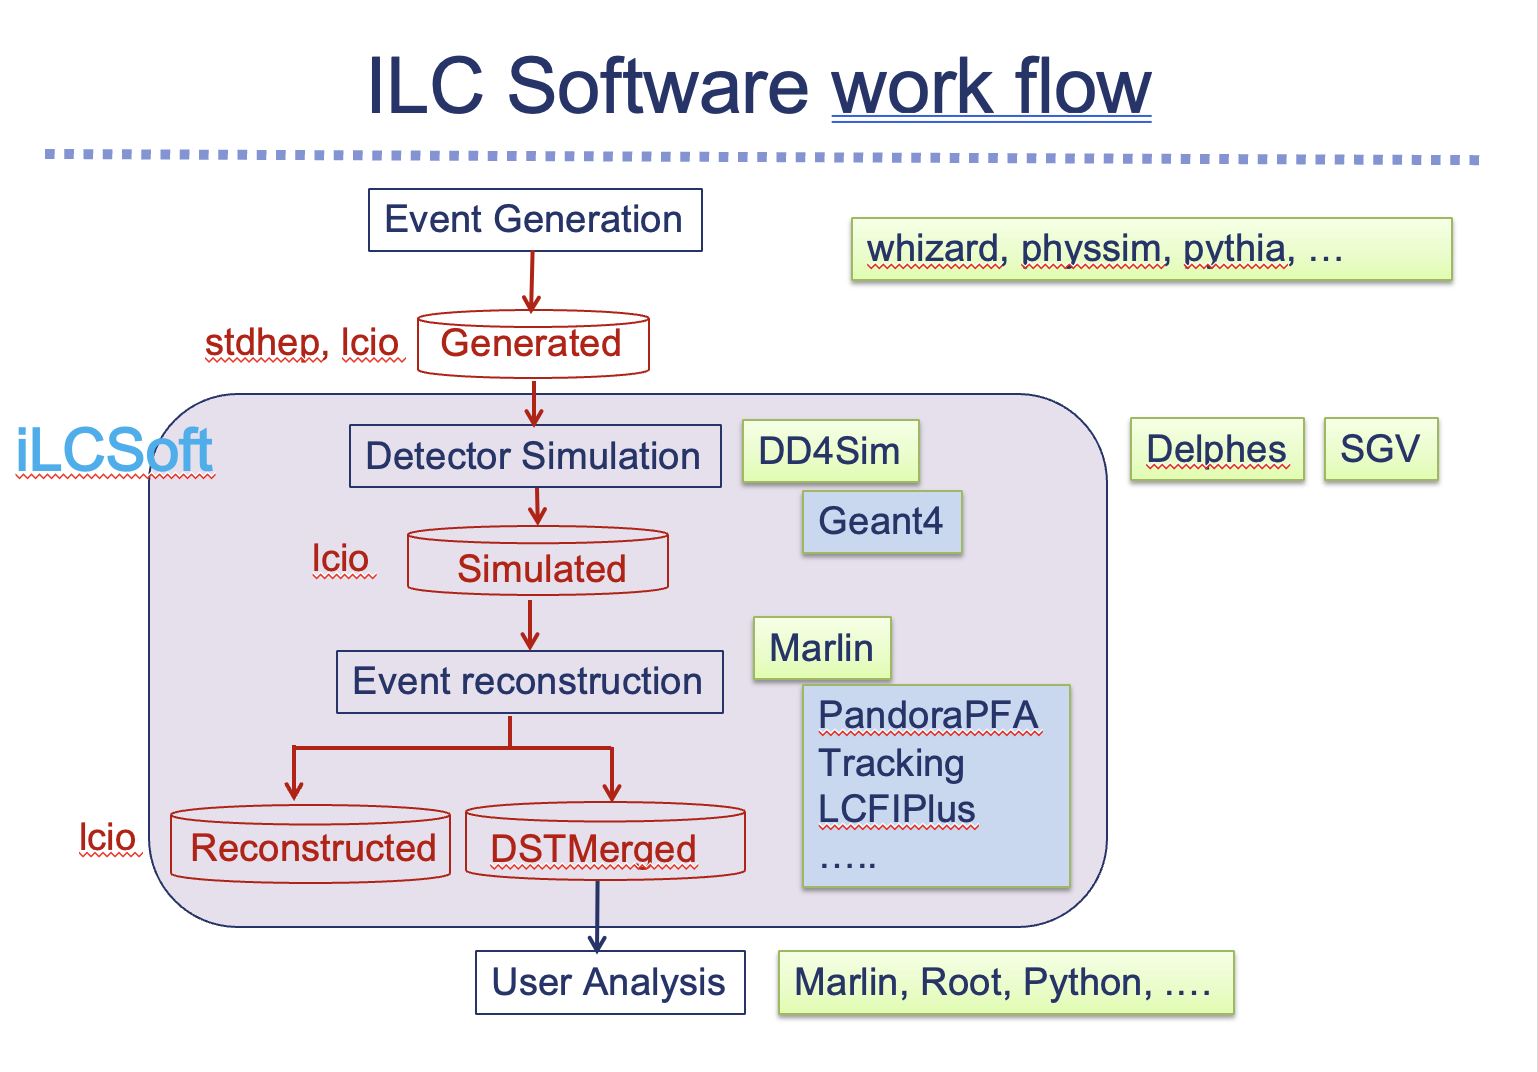
\includegraphics[width=370pt]{./Figure/EcalDetector/workflow.png}
		\caption[ILC Software のワークフロー]{ILC Software のワークフロー}
		\label{iLCSoft_workflow}
	\end{center}
\end{figure}
\end{comment}

\subsection{PandoraPFA}
PandoraPFA~\cite{PandoraPFA}はILCへ向けて開発されたPFAのためのソフトウェアである。PandoraPFAによるカロリメータクラスタリングおよび再構成はカロリメータにおけるヒットの情報やTPCにおける飛跡情報などを元にして行われる。一連の流れを示した図\ref{PandoraPFA}を示す。飛跡の情報はカロリメータのクラスタとマッチングするために用いられる。。カロリメータヒットの情報は3次元空間における位置、エネルギー損失、ECALおよびHCALのレイヤー番号を入力として使用する。入力されたヒットのうち、エネルギー損失が一定のヒットは削減され、その他のヒットはECALかHCALかで異なる較正係数を用いてエネルギー較正が行われる。%次に、ヒットのタグ付けに移る。あるヒットの周囲のヒットが基準値よりも低く、同じ層の隣接したセルでヒットが必要以上に存在していない場合に、そのヒットがMIPであると推定される。
PandoraPFAにおけるクラスタリングは各レイヤーごとのヒットから計算されるコーン角に基づいて計算される。まず、ビーム衝突点に近いレイヤーから順にカロリメータのヒット$i$がひとつ前のレイヤーのヒット$j$と比較される。
%二つのヒットの距離$\mathbf{r}_{ij}$とひとつ前のレイヤーのヒットから次のレイヤーのヒットへの向きを持つ単位ベクトル$\hat{\mathbf{u}}$を用いて、$d_\parallel = \mathbf{r}_{ij}\cdot \hat{\mathbf{u}}$および$d_\perp=\mathbf{r}_{ij}\times \hat{\mathbf{u}}$を計算する。これらのヒットのうち、コーンカット条件$d_\parallel < d_\perp \tan A + bD_{\textrm{pad}}$を満たすヒットを探索する。この時、$A$の2倍の値をコーン角と呼び、$D_{\textrm{pad}}$はセンサーのピクセルサイズを指す。

1つのヒットを頂角とする円錐領域の中に存在する次のレイヤーのヒットを考え、この円錐の開き角をコーン角と呼ぶ。カロリメータのヒットの一つ前の層のタグ付けされたヒットから、特定のコーン角を持つヒットに対して関連付けを行えるかどうか検索を行い、その層に候補となるヒットがなければさらに前へと遡って検索が行われる。これを繰り返すことでクラスタの種とそのクラスタに属するヒットが紐づけられる。この操作はECAL前面のヒットから外側のヒットへと順次行われる。
その後、飛跡がすでに紐づけられているクラスターに対して飛跡と紐づけられていないクラスターとのマージを行う。このマージはループした飛跡や途中で途切れている飛跡など、飛跡のトポロジカルな情報をもとにして行われる。

ここまでの解析はエネルギーロスが$\SI{50}{GeV}$以下の比較的クラスタリング性能の良いジェットに対して行われた。それ以上の高いエネルギーを持つジェットに対してはオーバーラップによる再構成のミスが生じる可能性があるため、クラスターのエネルギーが飛跡のエネルギーと一致するまで繰り返しクラスターを分割し、クラスタリングアルゴリズムを修正する。

再構成されたクラスターに対して光子同定アルゴリズムを適用し、光子から生じたクラスターを特定する。最後に、中性クラスターをクラスターと飛跡の距離に基づいて同定する。ここまでで得られた情報はParticle Flow Objects (PFOs)として保存される。

\begin{figure}[b]
	\begin{center}
		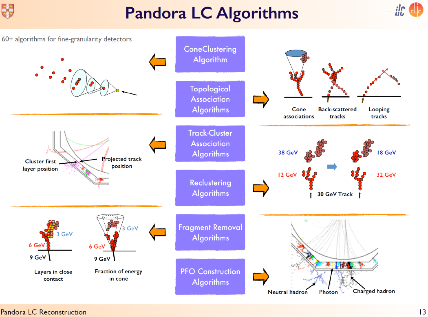
\includegraphics[width=200pt]{./Figure/EcalDetector/PandoraPFA_2.png}
		\caption[PandoraPFA のワークフロー]{PandoraPFA のワークフロー}
		\label{PandoraPFA}
	\end{center}
\end{figure}

現在のPandoraPFAのエネルギー分解能の性能を図\ref{PandoraPFA_res}に示す。カロリメータの単一ジェットに対するジェットエネルギー分解能を比較しており、このうち黒い実線はPandoraPFAを適用した時の性能である一方、赤い点線はPandoraPFAを適用していない場合の性能となっている。主に$\SI{100}{GeV}$以下の領域においてPandoraPFAを適用した場合の性能が良い分解能を示しているのがわかる。先行研究によりCalorimeterのみの場合のジェットエネルギー分解能性能は赤い点線で示された50-60\%$/\sqrt{E(\SI{}{GeV})}$である一方でPandoraPFAを適用した場合の性能は$\sim30\%/\sqrt{E(\SI{}{GeV})}$と改善しうることが示されている。しかし、その一方でカロリメータの分解能とジェット中の粒子の比から導出される理想的にPFAを適用した場合のジェットエネルギー分解能は$\sim20\%/\sqrt{E(\SI{}{GeV})}$と計算されており、PandoraPFAをさらに改善する余地があることが示唆されている。

\begin{figure}[H]
	\begin{center}
		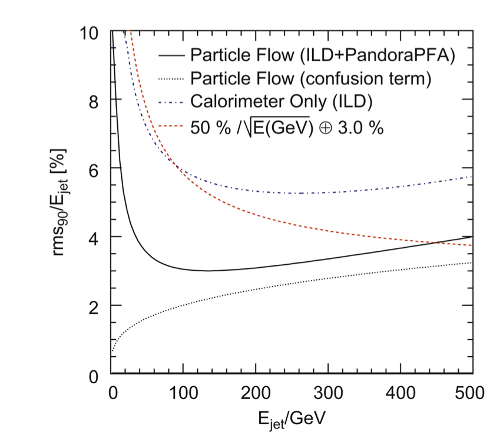
\includegraphics[width=250pt]{./Figure/EcalDetector/PFA_per.png}
		\caption[PandoraPFA を利用した場合のジェットエネルギー分解能]{PandoraPFA を利用した場合のジェットエネルギー分解能とその他の場合の比較。縦軸はエネルギー分解能を示し、小さいほど性能が良いことを示す。横軸はジェットのエネルギーである。例えば、50\%/$\sqrt{E}$という値は$\mathrm{E}_{\mathrm{jet}}$=$\SI{1}{GeV}$の時のエネルギー分解能と一致する。}
		\label{PandoraPFA_res}
	\end{center}
\end{figure}

%\subsection{PandoraPFAによるジェットエネルギー再構成性能}
%PandoraPFAを用いた際のジェットエネルギー分解能がシミュレーションデータを用いて評価された。\cite{PFATest}


%\subsection{プラスチックシンチレータ}
%シンチレータは光子検出を行うための検出器である。シンチレータに含まれる原子は光子の入射によって二次電子の放出を行い、二次電子が原子核に束縛されている電子に対して伝導体への励起を促す。しかし、二次電子によって伝導帯へと移動した電子は十分な時間が経過すると再び価電子帯へと遷移する。この際に伝導帯と価電子帯のエネルギー差に相当するシンチレーション光が発生する。通常、シンチレーション光を検出する検出器に対して波長が最適となるように、不純物をドープすることで中間準位を形成し、調整を行う。





 % !TEX root = ../MasterThesis.tex

\chapter{深層学習の概観} \label{sec:DeepLearning}
本章では、深層学習技術について、その概観を述べる。
3.1節では基本的な深層学習の概観を述べる。%3.2節では深層学習と粒子物理学との関連について取り上げる。
3.2節でグラフニューラルネットワーク(Graph Neural Network, GNN)について紹介した後、3.3節で一般的なニューラルネットワーク(Neural Network, NN)の実装について説明する。

%この章では、PFAを改善させるために導入した深層学習技術について、その概観を説明する。3.1節では深層学習の対象として教師あり学習と教師なし学習の違いを説明する。3.2節では深層学習の最も基本的な構造であるパーセプトロンについて述べる。3.3節ではパーセプトロンを組み合わせることで構成される単純な深層学習ネットワークであるニューラルネットワークについて述べる。3.4節では、ニューラルネットワークを使用する際の学習の進行過程について述べる。3.5節ではニューラルネットワークを用いる際に、さらに精度を向上させるための種々の技術について述べる。3.6節ではニューラルネットワークをさらに応用したグラフニューラルネットワークについて説明する。

\section{深層学習}
%21世紀以降、情報処理技術や微細集積回路製造技術などの発達により取り扱うデータや解析により得られるデータは膨大かつ複雑になっている。

21世紀以降、取り扱うデータや解析により得られるデータは膨大かつ複雑になっていることが課題となっており、それまでの技術では処理に必要となるアルゴリズムが要求される性能に対して不十分となるケースが増えている。したがって新たな解析手法が必要となっており、その一つとして研究されてきたのが深層学習技術である。深層学習は機械学習の一種であり、この後に紹介するディープニューラルネットワーク(Deep Neural Network, DNN)だけでなく、敵対生成ネットワーク(Generative Adversarial Networks, GAN)やAuto-encoderなども深層学習技術に含まれる。深層学習技術の特徴としては、入力されてきたデータの特徴をより詳細に、より様々な観点から捉えるために、「深い」構造を持っていることが挙げられる。%機械学習の構想は人間の知能と同等の能力を保持する計算機として開発が期待されていた人工知能というアイデアに影響を受けているが、人間の頭脳のように複雑な構造を計算機上でアルゴリズムとして再現するために深層学習技術はより深く、より多くのデータ量を扱えるように進歩してきた。

深いネットワークを構築することで表現能力が上がり、より複雑な問題を扱うことができるようになる。これにより従来よりも速い処理速度で解析を行う精度の高いアルゴリズムを作成することが可能となった。
%この特徴の長所として、アルゴリズムに新たな構造を加えるのではなく、基本的な構造をより深くすることで従来の技術では到達できなかったデータ量の解析を行うことが期待される点である。これにより新たなアルゴリズムを考案することなく、アルゴリズムに含まれるパラメータの数を変更することで性能の向上が見込める。

深層学習の例として、図\ref{DNN}のように表され、入力層と出力層に多数の中間層を挿入したネットワークであるDNNを取り上げる。この技術は教師あり学習として利用され、回帰問題や分類問題に使用される。

\begin{figure}[h]
	\begin{center}
		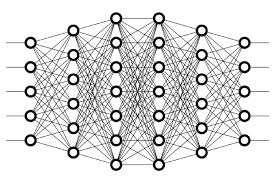
\includegraphics[width=250pt]{./Figure/DeepLearning/dl.jpeg}
		\caption[全結合DNNの模式図]{全結合DNNの模式図。}
		\label{DNN}
	\end{center}
\end{figure}


ここで、丸で表されている部分をノード、それらをつなぐ線をエッジと呼ぶ。エッジは各ノード間のパラメータを伝播し、ノードにおいてそのパラメータを元にした計算が行われているという過程が生じている。

入力として複数のベクトルからなるデータを考える。入力層と出力層の間では重み$\textbf{W}=\{\{w^0_1, w^0_2,\ldots, w_n^0\},\{w_1^1,w_2^1,\ldots ,w_n^1\},\ldots\}$とバイアス$\textbf{b}=\{b^0,b^1,\ldots\}$、そして非線形関数$h(x)$を通じた以下の計算が行われる。ただし、入力されたベクトルを$\textbf{x} = \{\{x^0_1, x^0_2,\ldots, x_n^0\},\{x_1^1,x_2^1,\ldots ,x_n^1\},\ldots\}$としている。
\begin{equation}
\textbf{y}  = h(\textbf{a}) = h(\textbf{Wx} +\textbf{b})
\end{equation}
ここで、重み$\textbf{W}$はサイズとして中間層の数と入力パラメータの数をもつ行列であり、その入力パラメータの寄与がどのくらい大きいかを表す一方、バイアス$\textbf{b}$は伝播してきたパラメータがどのくらい大きな寄与を示せば出力層へと伝播していくかの閾値を示しているとみなせる。また、ここで用いられている非線形関数を特に活性化関数と呼ぶ。

\begin{comment}
\begin{aligned}
\ h(\textbf{Wx} +\textbf{b})\\
\ h(\textbf{Wx} +\textbf{b})\\
\end{aligned}
\right.
\end{comment}

活性化関数についてはさまざまなものが提案されている。例えば、Rectified Linear Unit(ReLU)関数は
\begin{equation}
y = h(\textbf{a}) = \left\{
\begin{aligned}
0  \ (\textbf{a}  \le \theta)\\
\textbf{a}  \ (\textbf{a}  > \theta)\\
\end{aligned}
\right.
\end{equation}
と表され、入力が閾値を超えた後は入力に対して線形に増加する。他にも、双曲線関数$\tanh(\textbf{a})$やシグモイド関数$1/(1+\exp(-\textbf{a}))$などが用いられる。
これらの活性化関数を図\ref{act}に示す。

\begin{figure}[H]
	\begin{center}
		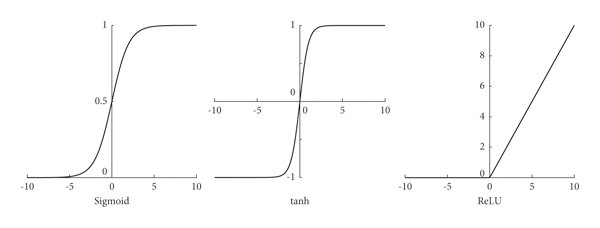
\includegraphics[width=350pt]{./Figure/DeepLearning/Output.jpeg}
		\caption[活性化関数の例。]{活性化関数の例。}
		\label{act}
	\end{center}
\end{figure}

深層学習の目的として、大きく分類問題と回帰問題の2種類が挙げられる。

分類問題は特徴量を持ったデータからそれぞれをいくつかの種類に識別する問題である。例として、手書き数字の画像を0から9までの数字に識別するMNIST問題が挙げられる。この課題では白黒、つまり0か1の数字で表現された手書き数字を離散的な出力$0~9$として分類する。

回帰問題はデータの特徴からその傾向について探り、連続的な変数を出力として得る問題である。

%どちらの種類の課題に対しても、深層学習は中間層を増やすことで表現能力が上がり、より多くの問題に対応できるようになるという特徴を持つ。

\section{Graph Neural Network}
Graph Neural Network (GNN)は深層学習技術の一つであり、グラフ構造を持ったデータの学習に有効であるという結果が得られている。グラフ構造を持ったデータは、DNNの説明でも述べたノードとエッジから構成されている。

グラフの構造として、いくつかの選択肢が存在する。
\begin{itemize}
\item エッジの向きの有無

2つのノードをつなぐエッジに対しては向きを設定することができる。向きを持ったグラフを有向グラフと呼び、持っていないものを無向グラフと呼ぶ。

通常、方向を持ったエッジはそうでないエッジに比べて情報量が多く、順方向と逆方向とで異なる特徴量を学習する。

\item グラフのノードの種類

全てのノードおよびエッジの種類が同じものを同種グラフ、複数の種類が混在しているものを異種グラフと呼ぶ。

\item 時間の経過に伴うグラフの変化

学習によってグラフの構造が変化する場合を動的グラフ、そうでない場合は静的グラフと呼ばれる。

\end{itemize}

また、学習を行う対象として幾つかの種類が存在する。
\begin{itemize}
\item ノードレベル 

各ノードを分類したり、ノード回帰の計算を行う。

\item エッジレベル

エッジごとの種類を分類するエッジ分類やエッジが存在するかしないかを予測するリンク予測などが挙げられる。

\item グラフレベル

グラフ全体の分類や回帰問題に関する問題を取り扱う。
\end{itemize}


GNNはノードとエッジの関連性に着目し、その特徴と関係性を学習することでグラフデータの解析を行うことが可能となる。応用例として、グラフベースで扱うことのできる化合物・生物分子解析、論文ごとの関連性、交通・物流予測などにおいて活用が図られている。

素粒子実験の分野ではグラフベースで扱えるものが少なくなく、現在GNNによる物理解析の研究が盛んになりつつある。例として、飛跡検出器で捉えられたヒットをノードに、飛跡をエッジとして考えることで検出器応答をグラフとして表せる。与えられたデータの特徴量をグラフとして与えるためには、グラフ構造の設計を考え適切なものを選択する必要がある。その際、ノードとエッジとして表現される対象に応じてGNNアーキテクチャの構造を選択することで最適な精度を得ることができる。


\section{ニューラルネットワークの実装}
GNNに限らず、ニューラルネットワークの実装には以下のいくつかの手順が必要となる。

\begin{enumerate}
\item データ準備

入力データは解析の精度を高める上でも重要であり、GNNの場合はグラフの形状に合わせたデータセットを用意する必要がある。深層学習においては前処理としてデータを$[-1,1]$の範囲に制限することでより精度の高い解析が可能となるケースが多い。

データは訓練データ、評価データに分割し、それぞれ別々の用途に用いる。

\item モデル作成

目的とするタスクおよびデータの特徴に応じた適切なネットワークモデルを選択する。

GNNの一つとして、計算の高速化と汎用化のために開発されたのがMessage Passingと呼ばれるネットワークである。
以下、入力パラメーターによってノード特徴量$x_v$、エッジ特徴量$e_{vw}$をもつ無向グラフGが構成されたとする。学習ステップを$\{t|t\in T\}$で表す。それぞれのノードには隠れ状態$h_v^t$が設定されており、Message Passingでは
\begin{equation}
m_v^{t+1} = \sum_{w \in N(v)} M_t(h^t_v,h^t_w,e_{vw})
\end{equation}
\begin{equation}
h_v^{t+1} = U_t(h_v^t,m_v^{t+1})
\end{equation}
のようにグラフの特徴量を伝達し、パラメータを更新する。

ここで、$N(v)$はインデックスvを含むノードおよびエッジに接続されている要素を示し、$M_t$および$U_t$はネットワークに固有の関数であり、それぞれメッセージ関数とノード更新関数と呼ばれる。

最終的な出力は読み出し関数$R$を用いて
\begin{equation}
\hat{y} = R(\{h_v^T | v \in G\})
\end{equation}
と得られる。

関数$M_t$、$U_t$、$R$は全てネットワークの学習によって得られる関数であり、隠れ状態$h_t$を通じて入力パラメータから得られる。
Message PassingはGraph Convolutional Networks(GCN)やNeural Fingerprint(NF)といったその他のGNNの構造をこれらの関数によって一般化したものと考えられる。

例えば、Convolutional Networkの1つはMessage Passingにおいて
\begin{equation}
M(h_v,h_w,e_{vw}) = \mathrm{concatenate}(h_w,e_{vw})
\end{equation}
\begin{equation}
U_t(h_v^t,m_v^{t+1}) = \sigma(H_t^{\mathrm{deg}(v)}m_v^{t+1})
\end{equation}
(ただし、$\sigma$はシグモイド関数、$\mathrm{deg}(v)$はノード$v$の数、$H_t^N$はステップ$t$、ノード数$N$の時の学習によって得られた行列を指す。)
\begin{equation}
R = f(\sum_{v,t} \mathrm{softmax(W_th_v^t)})
\end{equation}
(ただし、$f$はニューラルネットワーク、$W_t$は学習によって得られた読み出し行列を指す。)

のように関数を定義した場合と同様である。

ネットワークとしてBatch Normalizationと呼ばれる手法を用いることがある。この手法はレイヤーごとに特徴量を規格化することで過学習を避けるための方法となっている。まず、出力されてきたバッチから平均と分散を計算する。出力を$x_i$、出力の数を$m$とすると、平均$\mu_B$および分散$\sigma_B^2$は
\[
\mu_B = \frac{1}{m}\sum_{i=1}^m x_i
\]

\[
\sigma_B^2 = \frac{1}{m}\sum_{i=1}^m(x_i-\mu_B)^2
\]

となり、この値を用いて出力として
\begin{equation}
\hat{x_i} = \frac{x_i - \mu_B}{\sqrt{\sigma_B^2+\epsilon}}
\end{equation}
のように規格化される。
ここで分母に微少量$\epsilon$を加えることにより$\sigma_B^2$が小さくなってしまいゼロ除算が発生することを防いでいる。
こうして求められたバッチデータに対して線形変換
\begin{equation}
y_i\leftarrow\gamma\hat{x_i}+\beta
\end{equation}
を行うことで、平均$\beta$、標準偏差$\gamma$の正規分布が得られる。

\item モデル学習

学習に必要となる損失関数とその最適化手法を決定し、実行する。
損失関数とはネットワークから出力されてきた数値と正解ラベルとのズレを示す関数であり、NNからの出力を$y_k$、正解ラベルを$t_k$とすると回帰問題に使用される二乗和誤差関数(Mean Squared Error)
\[
L=\frac{1}{2}\sum_k (y_k-t_k)^2
\]
と分類問題において使用される交差エントロピー誤差(Cross Entropy Error)
\[
L=-\sum_k t_k\log(y_k)
\]
が主に挙げられる。

損失関数$L(\textbf{W})$の重みパラメータ$\textbf{W}$による勾配を得るために取られる有用な手法が誤差逆伝播法である。

\begin{comment}
順方向のニューラルネットワークの計算は
\[
\textbf{y} = h(\textbf{Wx} + \textbf{b}) 
\]
であったが、
\end{comment}
%勾配を計算するためには$\textbf{W}$と$\textbf{x}$が必要である。
順方向の損失関数までの伝播を模式的に表したものを図\ref{BackProp}に示す。
なお、この図は計算グラフと呼ばれるニューラルネットワークの計算の過程を視覚的なグラフで表したものである。

\begin{figure}[H]
	\begin{center}
		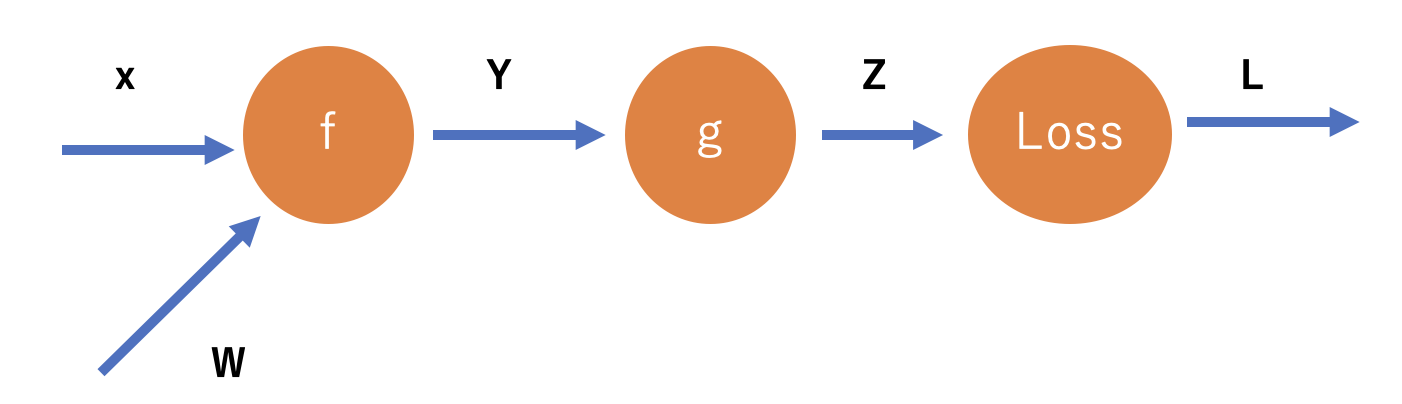
\includegraphics[width=350pt]{./Figure/DeepLearning/BackProp.png}
		\caption[順方向の伝播を示す計算グラフ]{順方向の伝播を示す計算グラフ。}
		\label{BackProp}
	\end{center}
\end{figure}

計算グラフはこれら一連の計算によって損失関数$L$が
\begin{equation}
L = \textrm{Loss}(g( f(\textbf{x}, \textbf{W}))) = \textrm{Loss}(g(\textbf{Y})) = \textrm{Loss}(\textbf{Z})
\end{equation}
と順々に計算されている様子を表している。

%ニューラルネットワークでは$f(x)$は関数$f(\textbf{W}, \textbf{x}) =\textbf{W}\textbf{x}$、$g(x)$は関数$g(\textbf{W}\textbf{x}, \textbf{b})=\textbf{W}\textbf{x}+\textbf{b}$、そしてLossはシグモイド関数などの非線形関数に対応する。

%非線形関数$h(x)$からの出力をそれぞれ$\textbf{Y}$、$\textbf{Z}$とし、ロスを$L$とすると
今回、損失関数$L$の重み$\textbf{W}$に対する勾配を考えたいので、各出力による微分を考える。この際、誤差逆伝播法によると$\textbf{x}$、$\textbf{W}$、$\textbf{Y}$、$\textbf{Z}$に対する逆伝播はそれぞれ図\ref{BackProp_back}のように表される。

\begin{figure}[H]
	\begin{center}
		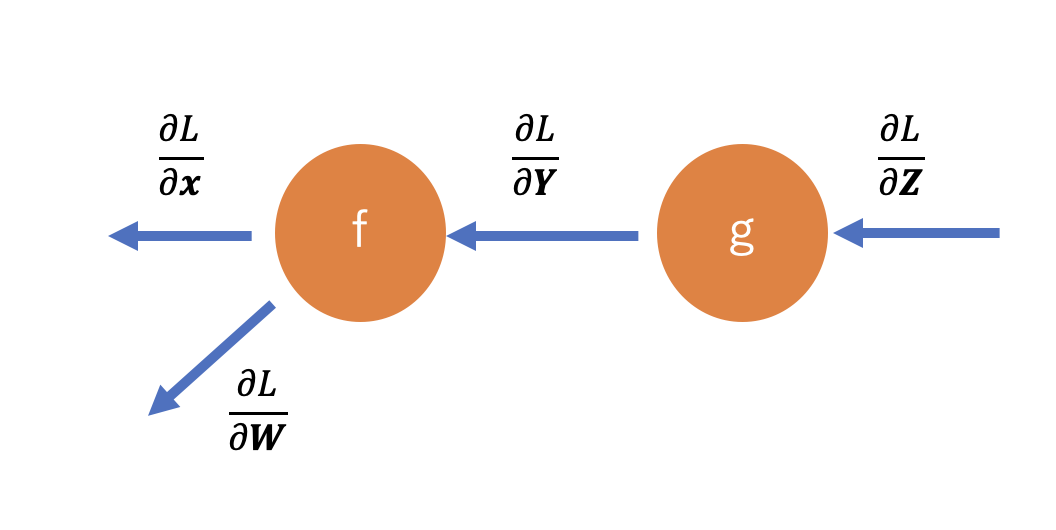
\includegraphics[width=350pt]{./Figure/DeepLearning/BackProp_back.png}
		\caption[逆伝播の模式図]{逆伝播の模式図}
		\label{BackProp_back}
	\end{center}
\end{figure}

1つのノードから2本の有向エッジが伸びている場合に、一方を計算するためにはもう片方のエッジとノードに入力されてきたエッジとの積を計算する。
すなわち、勾配$\frac{\partial L}{\partial \textbf{W}}$を得るためには
\begin{equation}
\frac{\partial L}{\partial \textbf{W}} = \frac{\partial L}{\partial \textbf{x}} f\left(\frac{\partial L}{\partial \textbf{Y}}\right)
\end{equation}
を計算する。
よって、求めたい勾配は損失関数から
\begin{equation}
\frac{\partial L}{\partial \textbf{W}}= \frac{\partial L}{\partial \textbf{x}}\cdot f\left(g\left(\frac{\partial L}{\partial \textbf{Z}}\right)\right)\end{equation}
と得られる。
なお、合成関数の微分から、右辺は
\begin{equation}
\frac{\partial L}{\partial \textbf{W}} = \frac{\partial }{\partial \textbf{x}}\left(f\left(g\left(\frac{\partial L}{\partial \textbf{Z}}\right)\right)\right)
\end{equation}
とも表される。

勾配を得るための方法として、重みパラメータそれぞれに関して損失関数の数値微分を行うことも可能だが、計算が非常に膨大になるため、実用的には誤差逆伝播法が用いられる。

最適化手法の一つとして、RMSPropを説明する。
誤差逆伝播法の結果から、
%重み$\textbf{w}^{(t)}$に依存した損失関数$L(\textbf{w}^{(t)})$が得られたので、
この損失関数の勾配$\textbf{g}^{(t)}$に沿って損失関数を低減させることでネットワークから出力されてきた値を正解ラベルへと近づけることができる。

勾配$\textbf{g}^{(t)}$は
\[
\textbf{g}^{(t)} = \Delta L(\textbf{W}^{(t)})
\]
である。RMSPropでは、パラメータ$\textbf{v}_{(t)}$を導入し、重みパラメータを更新する前に
\[
\textbf{v}_{(t)}=\rho\textbf{v}_{(t-1)}+(1-\rho)(\textbf{g}^{(t)})^2
\]
を計算する。
この$\textbf{v}_{(t)}$を用いて重みパラメータの勾配$\Delta\textbf{W}^{(t)}$を
\[
\Delta\textbf{W}^{(t)}=-\frac{\eta}{\sqrt{\textbf{v}_t+\epsilon}}\textbf{g}^{(t)}
\]
と計算し、新たな重みパラメータ
\[
\textbf{W}^{(t+1)} = \textbf{W}^{(t)}+\Delta\textbf{W}^{(t)}
\]
が得られる。RMSPropは先に行われていた重みパラメータの更新が後のパラメータ更新へ影響を与えにくくなるため、学習の間で勾配変化の大きい場合の学習に適している手法である。これを応用してAdamやAdamWといったさまざまな最適化手法が考案されている。


\begin{comment}
合成関数の微分と最適化アルゴリズムを用いて得られた$\Delta\textbf{W}^{(t)}$を用いて
\frac{\partial L}{\partial y_{ij}} = \sum_{k,l}\frac{\partial L}{\partial z_{kl}} \frac{\partial z_{kl}}{\partial y_{ij}}
\end{comment}


\begin{comment}
\[
 \frac{\partial E}{\partial w_{jk}} = h'_k(w_k x_k)\frac{\partial E}{\partial y_k}y_j
\]
を得る。ただし、$w_{jk}$は重みパラメータ$\textbf{W}$のjk成分。$x_j$および$x_k$$y_j$および$y_k$はそれぞれ出力$\textbf{x}$、$\textbf{y}$のj,k成分。
\end{comment}



%選択されたモデルによって出力が得られた後、損失関数の計算が行われ、最適化手法によりパラメータが調整される。全てのデータを用いてパラメータが調整されるタイミングが1エポックと呼ばれ、学習回数を表す単位の一つとなる。



\item モデル評価

訓練データ、評価データを用いてネットワークの評価を行う。
\begin{itemize}
\item 推論性能評価

全ての評価データのうち、正しくネットワークが判別できているデータの割合を推論精度(Accuracy)と呼び、ネットワークによる推論の確らしさを示している。
\item  汎用性能評価

訓練データと評価データに対する損失関数の学習進度ごとの変化から、汎化推論精度を確認することができる。訓練データのみの損失関数が減少している場合、ネットワークの汎化性能は低いと言える。なお、学習進度を示す単位として、訓練データを何回繰り返したかをエポック(epoch)と呼ぶ。

\end{itemize}

\end{enumerate}










%%%%%%%%%%%%%%%%%%%%%%%%%%%%%%%%%%%%%%%%%%%%
\begin{comment}
\subsection{教師あり学習と教師なし学習}
機械学習は与えられた特定のデータから目的とする正解データをアルゴリズムにより導くための技術である。深層学習は深層ニューラルネットワークを利用した機械学習技術の一部に位置づけられる。機械学習の対象となる課題には、教師あり学習と教師なし学習に分けられる。教師あり学習では、まず入力となるパラメータと正解ラベルを持つデータが与えられ、その相関関係を元にして目的となるデータの予測ラベルを出力する。一方、教師なし学習では正解ラベルを与えられることなしに入力パラメータのみから予測ラベルの推定を行う。今回目的とするカロリメータークラスタリングのような解析は前者が有効となる。他方でロボットの制御やビデオゲームにおける最適行動解の探索などには強化学習として、後者が用いられることがある。


\subsection{単純パーセプトロン}

単純パーセプトロンは図のような入力層と出力層のみを持つ単純なネットワークである。このネットワークに入力パラメータを$x_1$、$x_2$が与えられると、重み$w_1$、$w_2$を乗算して和をとった$w_1x_1+w_2x_2$が計算され、出力層には非線形関数$h(x)$を通じて出力$y$が求められる。$h(x)$は単純パーセプトロンの場合はヘヴィサイドの階段関数と呼ばれる閾値$\theta$を持った関数が用いられ、
\begin{equation}
y = h(a) = \left\{
\begin{aligned}
0  \ (a = w_1x_1 + w_2x_2 \le \theta)\\
1  \ (a = w_1x_1 + w_2x_2 > \theta)\\
\end{aligned}
\right.
\end{equation}
ここで、重み$w_1$、$w_2$はその入力パラメータの寄与がどのくらい大きいかを表し、バイアス$\theta$はそのパラメータがどのくらい大きな寄与を示せば出力層へと伝播していくかの閾値を示しているとみなせる。また、出力層に伝播する際に使用される非線形関数を特に活性化関数と呼ぶ。一層だけの単純パーセプトロンでは極めて限られたケースしか取り扱えないがこれらを組み合わせることで、次の節で紹介するニューラルネットワークとして応用範囲を広げることができる。


\subsection{ニューラルネットワーク}
中間層を増やすことで表現能力が上がり、より多くの問題に対応できるようになっている。重みの計算は単純パーセプトロンの場合と同様だが、出力層において用いられる非線形関数についてさまざまなものが提案されている。例えば、Rectified Linear Unit(ReLU)関数は
\begin{equation}
y = h(a) = \left\{
\begin{aligned}
0  \ (a  \le \theta)\\
a  \ (a  > \theta)\\
\end{aligned}
\right.
\end{equation}
と表され、入力が閾値を超えた後は入力に対して線形に増加する。他にも、双曲線関数$\tanh(a)$やシグモイド関数$1/(1+exp(-a))$などが用いられる。
中間層が多く存在するニューラルネットワークを深層ニューラルネットワークと呼び、このような深いネットワークを用いて学習することを特に深層学習としている。


\subsection{損失関数}

\subsection{誤差逆伝播}


深層教師あり学習には大きく分けて5つの段階が存在する。
\begin{itemize}
\item データをネットワークに適切な形式となるように整形する
\item 入力データをネットワークに入れてその出力と正解ラベルとの差を比較する
\item その差を元にして誤差逆伝播法によりネットワークの重みやバイアスを学習する
\item 上記2 - 3を誤差が最適となるまで繰り返す
\item 評価データを用いてネットワークの性能を評価する
\end{itemize}

これらの過程を通じて入力データから出力データの値を推定する。


\section{精度向上のための技術}
ニューラルネットワークの問題点の一部が勾配消失や過学習である。前者は損失関数を計算するときにその勾配計算ができなくなり、学習が進まなくなる現象である。一方、後者はネットワークが訓練データに適合しすぎて、評価データに対して適切に出力できなくなる問題である。特に深いネットワークでは、これらの問題が起こりやすい。解決策としては、バッチノーマリゼーションや重み初期値の変更、ハイパーパラメータチューニングが挙げられる。バッチノーマリゼーションは各レイヤーの間にバッチ層を挟み、入力されてきたパラメータを規格化するという手法である。また、学習を行う前のネットワークの重み初期値をXavierの初期値などを使うことで改善することもできる。さらに、ネットワークに含まれるレイヤーの数や学習率などのパラメータはハイパーパラメータと呼ばれ、学習の際には一意に決められている。このパラメータをさまざまに帰ることでネットワークの性能が変化しうる。この調整をハイパーパラメータチューニングと呼ぶ。


\section{グラフニューラルネットワーク}
グラフニューラルネットワーク(GNN)はニューラルネットワークにグラフの概念を利用することで、それぞれのデータの関係性がグラフによって表される場合に、その関係性を学習に活用することを可能にするネットワークである。グラフは各特徴量を保持するノードと、それぞれの特徴量の関係を表すエッジによって構成され、ノードの種類が同じグラフをホモジーニアス、異なるグラフをヘテロジーニアスと呼ぶ。応用例としてはグラフベースで扱うことのできる、化合物・生物分子解析、論文ごとの関連性、交通・物流予測などが挙げられる。
\end{comment}
%%%%%%%%%%%%%%%%%%%%%%%%%%%%%%%%%%%%%%%%%%%%%

 % !TEX root = ../MasterThesis.tex

\chapter{グラフニューラルネットワークによるクラスタリング解析} \label{sec:BeamTest}

本章では、カロリメータクラスタリングに対して適用したネットワークおよび損失関数に関する技術の概要を説明し、ILCの検出器シミュレーションに対して適用した際のクラスタリング性能について示す。
4.1節では、今回使用した深層学習アーキテクチャについてその全体像を説明する。4.2節では今回使用したネットワークであるGravNetについて述べる。4.3節では、クラスタリング性能を高めるために使用した Object Condensation技術について解説する。最後に、4.4節では近接する2光子イベントをILC検出器シミュレーションで作成し、そのクラスタリング性能を評価した。

\section{深層学習アーキテクチャ}
今回用いた深層学習アーキテクチャを図\ref{GravArc}に示す。
\begin{figure}[H]
	\begin{center}
		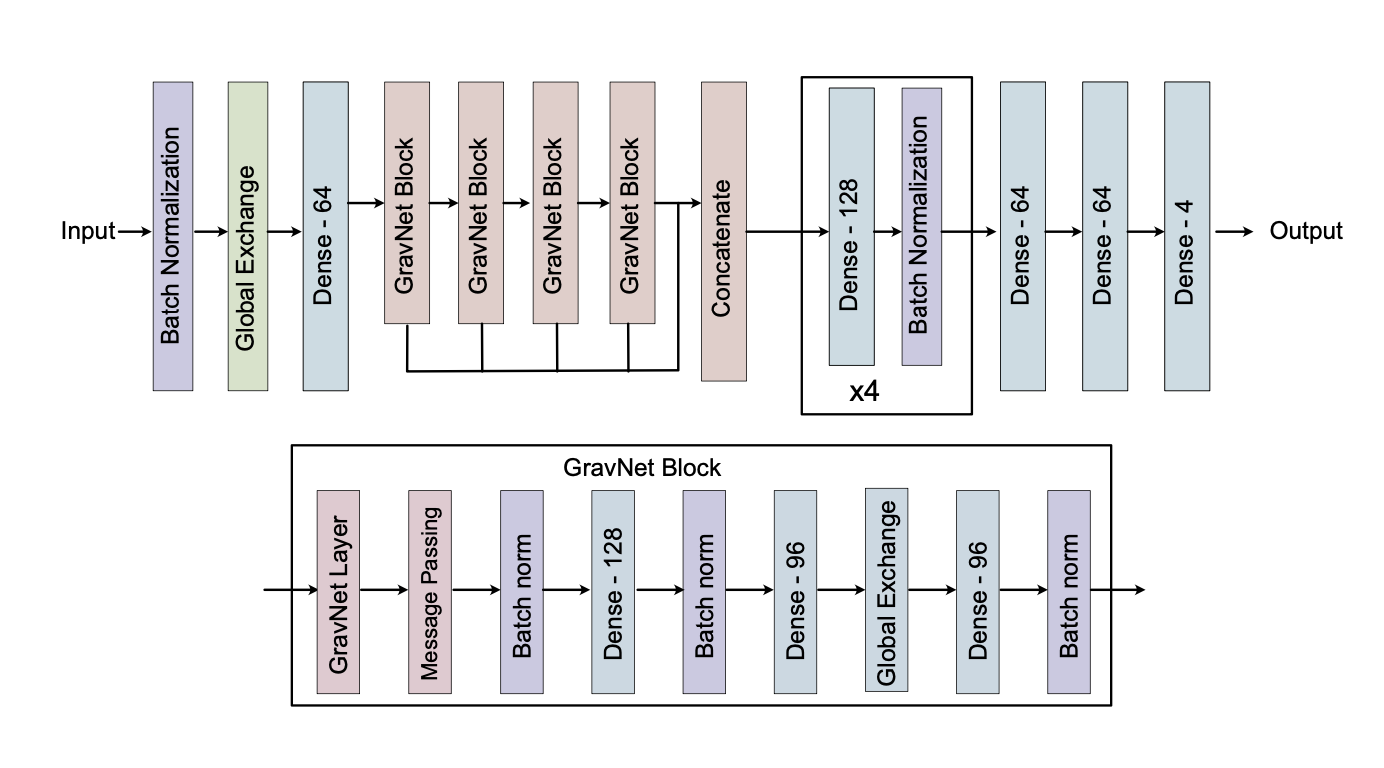
\includegraphics[width=300pt]{./Figure/DLAnalysis/GravArc.png}
		\caption[用いたGravNetアーキテクチャ]{今回用いたGravNetアーキテクチャ。}
		\label{GravArc}
	\end{center}
\end{figure}

入力されたパラメータはまずBatch Normalization, Global Exchange, Dense 層を通過して整形される。Batch Normalizationは過学習を避けるためにBatchごとの出力を規格化する過程である。また、Global Exchange ではバッチごと、特徴量ごとに平均値、最小値、最大値を抽出して入力されたパラメータとconcatenateし、次のレイヤーへと伝達している。これにより、入力されたヒット特徴量の最小や最大、平均といった特徴をより影響しやすくしていると考えられる。Dense層は式(3.1)で表される、線形項と非線形項を組み合わせた全結合層であり、深層ネットワークを構成する基本的な構造の一つである。

その後、GravNet Blockへと移行し、ここではGravNetおよびMessage Passing、 Batch Normalization、 Dense層を含む処理が行われる。GravNet Blockを4回通過した後、Dense 層とBatch Normalizationを同様に4回適用し、最後に3層のDense層を経て出力が得られる。
%このネットワークはGravNetおよびGlobal Exchange、Message Passing以外はヒットの特徴量のみを用いた操作であり、他のNodeとは結合していない。
活性化関数として、GravNet BlockではTanh関数、GravNet Blockの後のDense層ではReLU関数を利用している。また、最適化アルゴリズムとしてAdamWを用いた。これらのネットワーク構造の決定はハイパーパラメータの一種であり、データセットに応じて調整が必要である。


\section{GravNet}

本研究で利用したネットワークについて、その構造と特徴について説明する。

GravNet\cite{GravNet}は、LHCの測定器の一つ CMS (The Compact Muon Solenoid) において、HL-LHC (High Luminosity-LHC)アップグレードで導入される予定のHGCAL (High Granularity CALorimeter) を用いたカロリメータクラスタリングのために開発された深層学習ネットワーク\cite{GravNet_CMS}である。
%欧州原子核研究機構(CERN)の管轄するLHC (Large Hadron Collider)の衝突点付近に置かれる検出器CMS (The Compact Muon Solenoid) 

本研究では入力データとして、カロリメータにおけるヒットの位置およびエネルギー損失を利用する。ヒットの位置は3次元空間上の座標として表現されるので、各ヒットを表す特徴量は今回は4種類存在する。ネットワークに入力されたパラメータはまず全結合層を通過し、その出力をもとにグラフが構成される。全結合層の出力層は、一部はグラフを構成する表現空間の座標に対応し、残りは表現空間における特徴量として利用する。表現空間上の座標を$S$、特徴量を$F_{LR}$とおく。
%表現空間の次元を増やすとより広範な表現能力を獲得できるが、それが過剰になると過学習を起こす危険性が高まる。
ここでは表現空間をSとし、ヒットに対応するグラフのノードのラベルを $(j,k)$とする。ただし、注目するノードをインデックス$k$、そのノードとエッジによって結合したノードをインデックス$j$で表す。さらに、空間S中の2つのノード$(j,k)$間の距離を$d_{jk}$とすると、この距離$d_{jk}$が最も近い$N$個のノードが、エッジによって互いに結合している。

それぞれのノードは周辺のノードから以下の手順に従って特徴量を収集する。

\begin{enumerate}
\item  一つのノードに対して、結合されたノードに与えられた特徴量$f^{i}_{j}$およびノード間の距離$d_{jk}$から、特徴量
\begin{equation}
\tilde{f_{jk}^i} = f^i_j \times V(d_{jk})
\end{equation}
を計算する。ここで、$V(x)$は距離の長さを考慮したポテンシャルを表し、近くのノードほどその影響が大きくなるように設計されている。今回は$V(d_{jk})=\exp(-d_{jk}^2)$を用いた。この計算は一つのノードに対して、結合しているノードの数、すなわち$j$回だけ行われる。

\item 各ノードに対して$\tilde{f_{jk}^i}$を計算した後、それらを concatenate
\footnote{concatenateとは与えられた行列を任意の方向に連結する操作を指す。例として、
\[
A = \begin{pmatrix}
a_1&a_2\\
a_3&a_4\\
\end{pmatrix}
\]
および
\[
B=\begin{pmatrix}
b_1&b_2\\
b_3&b_4\\
\end{pmatrix}
\]
が与えられた時に、
\[
\mathrm{concatenate}(A, B)= 
\begin{pmatrix}
a_1&a_2&b_1&b_2\\
a_3&a_4&b_3&b_4\\
\end{pmatrix}
\]
もしくは
\[
\mathrm{concatenate}(A, B)= 
\begin{pmatrix}
a_1&a_2\\
a_3&a_4\\
b_1&b_2\\
b_3&b_4\\
\end{pmatrix}
\]
となる。
}

することで新たな特徴量$\tilde{f_k^i}$を得る。例えば、$j$個のエッジに対する和や最大値が考えられる。今回は以前行われた研究から得られた結果をもとにして、平均値を利用した。

\item  上記の結果を全てのノードに対して行うことで、$\tilde{f_{k}^i}$を行列要素としてもつ特徴量$\tilde{F_{LR}}$が得られる。この特徴量は入力時に作成された特徴量$F_{\mathrm{IN}}$ベクトルとconcatenateされる。この出力を$F_{\mathrm{OUT}}$と表す。
\end{enumerate}

これらの3つの操作を2回繰り返し、最終的に$F_{\mathrm{IN}}$、$F_{\mathrm{OUT}}$、$F_{\mathrm{OUT}'}$の3つがconcatenateされて出力として得られる。
最終的に計算された出力は各ヒットおよびグラフにより関連づけられたヒットの特徴を表していると考えられる。

\section{Object Condensation}
4.1節で述べた深層学習アーキテクチャを損失関数を用いて学習を行う。今回、アーキテクチャからの出力は$\beta_i$と座標、そしてクラスター特徴量の3種類に分けられている。これらの利用法については以下で述べる。

損失関数として、通常の方法よりも与えられた特徴をさらに効率的に利用するために Object Condensation\cite{GravNet_Object} と呼ばれる手法を用いた。ここで、Condensation pointとは、仮想空間上でそれぞれのクラスターに対して与えられる、それぞれのクラスターに属するヒットが集約する点であり、図\ref{ObjectCondensation}のように現れる。
\begin{figure}[H]
	\begin{center}
		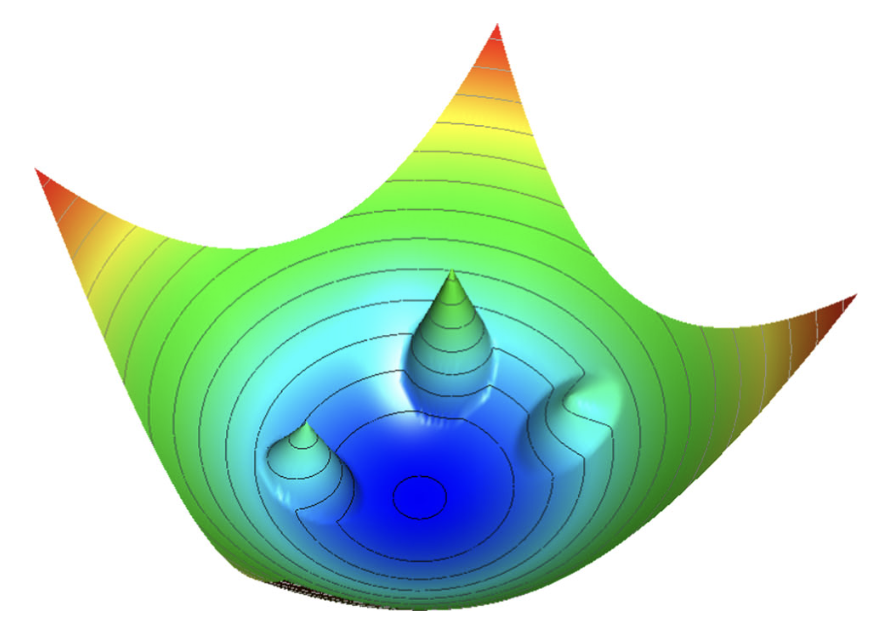
\includegraphics[width=250pt]{./Figure/DLAnalysis/oc.png}
		\caption[ObjectCondensation]{ObjectCondensation\cite{StandardModel}において$L_V$を構成するポテンシャルを模式的に描いた図。突起状に飛び出た部分がCondensation pointと呼ばれる。}
		\label{ObjectCondensation}
	\end{center}
\end{figure}

この手法では、損失関数として次の2つの項を採用し、クラスター識別性能を高めている。
\begin{equation}
L=L_V + L_p
\end{equation}

第一項は全ポテンシャル損失を表す。ネットワークから出力される値は、それぞれのヒットが正しいクラスターに属しているかどうかを示す$\beta_i$となっている。Object condensationはこの値をもとにノードの持つ電荷を定義し、ネットワークのパラメータ更新に用いられる。すなわち、
\begin{equation}
q_i =\arctanh^2\beta_i + q_{min}
\end{equation}
によって電荷$q_i$を定義する。特定のクラスター$k$に属するヒット$i$のもつ$q_i$はポテンシャル$V_{ik}$を有する。
電磁気学のアナロジーから、ヒットが正しいクラスターへ引力によって引き付けられ、誤ったクラスターから斥力によって離れるように学習を行いたい。
そのため、電荷$q_j$とポテンシャル$V_{ik}(x_j,q_j)$を用いて、各ヒットに働く静電気力を以下のように表す。

\begin{equation}
q_j \cdot \Delta V_k(x_j) = q_j \Delta \sum_{i=1}^{N} M_{ik} V_{ik} (x_j ,q_i)
\end{equation}

ここで、行列$M_{ik}$はヒット$i$がクラスター$k$に属している場合は1を、そうでなければ0を表す。この行列は$N\times N$個の要素数を持つので、全てのポテンシャルを計算するのは計算リソースの消費が大きくなるという問題がある。そのため、それぞれのクラスターに含まれるヒットの中から、以下のように最も大きなポテンシャルを持つヒット$i$のポテンシャルによって近似する。

\begin{equation}
V_k(x) \approx V_{\alpha k}(x, q_{\alpha k}),\  with\ q_{\alpha k} = \max q_i M_{ik}  
\end{equation}

すなわち、一つのクラスターのなかでそれぞれのヒットに働くクーロン力はその電荷にのみ依存する。

この表式を用いて、引力および斥力ポテンシャルは以下のように表される。
\begin{equation}
\check{V}(x) = ||x-x_{\alpha} ||^2 q_{\alpha k}
\end{equation}
\begin{equation}
\hat{V}_{k}(x) = \max(0,1-||x-x_\alpha ||)q_{\alpha k}
\end{equation}

前者のポテンシャルにより、それぞれのヒットは各クラスターに割り当てられた Condensation point$||x-x_{\alpha}||=0$へと集められる。一方、誤ったクラスターに近づいている場合は後者のポテンシャルによってそのクラスターから引き離される。斥力ポテンシャルに関して、ポテンシャルが大局的鞍点とは異なる局所的な平衡点へとどまりパラメータ更新が進みにくくなるのを防ぐためにポテンシャルと0を比較した時の最大値を採用した。

上記の2つの項を合わせて、損失関数のポテンシャル項は以下のように表される。
\begin{equation}
L_V = \frac{1}{N}\sum_{j=1}^{N} q_j \sum_{k=1}^K \left(M_{jk} \check{V}_k(x_j) + (1 - M_{jk})\hat{V}_k(x_j)\right)
\end{equation}

この損失関数は$||x-x_{\alpha}|| = 0$に鞍点をもち、同じクラスターに属するヒットはその中で最も電荷の高いヒットへと引っ張られる。一方、そのクラスターに属さないヒットは離れた位置へと押しやられる。

式(4.2)の第2項はベータ損失と呼ばれ、先ほど定義した各クラスターを代表するヒットの持つ$\beta$の値を最大化するために用いられており、以下で定義される。
\begin{equation}
L_\beta = \frac{1}{K}\sum_k (1-\beta_{\alpha k}) +s_B \frac{1}{N_B}\sum_i^N n_i \beta_i
\end{equation}
ここで、$s_B$はハイパーパラメータであり、データセットごとに異なる値を取る必要がある。この項の存在によって、それぞれのヒットのCondensation pointの影響が強調され、バックグラウンドやノイズの影響が低減される。$s_B$はバックグラウンドを低減させる強さを示し、全てのクラスターが正しくラベル付けされていれば大きく設定する。


\section{ILCの検出器シミュレーションデータを用いたカロリメトリー}
この章では、シミュレーションフレームワークの一つであるWHIZARDおよびILD検出器シミュレーション(iLCSoft v02-02)を用いて生成された2光子イベントのGravNetによるクラスタリングについて述べる。4.2.1節で入力データについて述べた後、4.2.2節でネットワークの評価を行う。

%%%%%%%%%%%%%%%%%%%%%%%%%%%%%%%%%%%%%%%%%%%%%%%%%%%%%%%%%%%%%%%%%%%%%%%%%%%%%%%%%%%%
\begin{comment}
\subsection{入力データ}
今回使用したデータは重心エネルギー$\SI{500}{GeV}$におけるZ粒子の崩壊を通じたハドロニック事象である。 シミュレーションにおいて、反応により生じた光子や中性ハドロンなどの粒子がILDのEcalおよびHcalへ入射し、電磁シャワーやハドロンシャワーを引き起こす。今回は1600事象を含むデータを用意した。

検出器シミュレーションにより出力されるのは各ヒットの位置、エネルギー損失やその生成元となるMC粒子の情報を持ったLCIOファイルである。LCIOファイルはPythonによって読み込みが可能であるが、深層学習を適用するためにはデータの剪定と事前処理が必要である。データを読み込む際に毎回この処理を行うと時間がかかりすぎるので、このファイルをPythonコードにより変換し、各事象ごとにnpzファイルを作成した。npzファイルにはヒットの情報として位置($x$,$y$,$z$)および各エネルギー損失が含まれる。ヒットの時間情報は今回は使用しなかった。正解ラベルとして、各ヒットが生成されたMC粒子のIDをもとにした番号を割り当てた。番号はMC粒子の種類に関わらず、0から昇順に生成された。

図\ref{Input}、\ref{EnergyDep}にある一つのイベントに含まれる各ヒットの位置およびエネルギー損失の情報を示す。ヒット位置のプロットに関して、原点がビーム衝突位置である。

\begin{figure}[H]
	\begin{subfigure}{.5\textwidth}
		\begin{center}
 		 	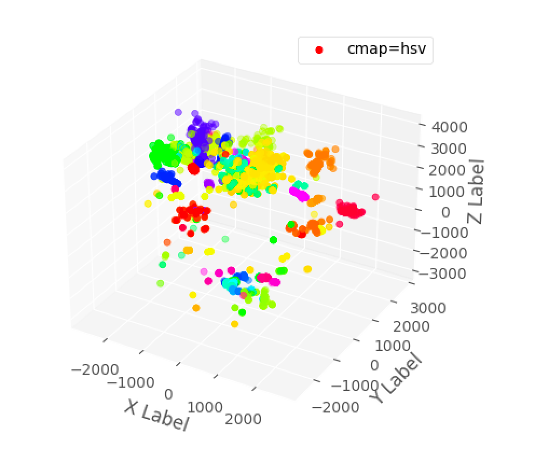
\includegraphics[width=200pt]{./Figure/DLAnalysis/Input.png}%.5\linewidth]{./Figure/DLAnalysis/Input2.png}
  			\caption{}
  			\label{fig:sfig1}
 		\end{center}
	\end{subfigure}
	\begin{subfigure}{.5\textwidth}
		\begin{center}
			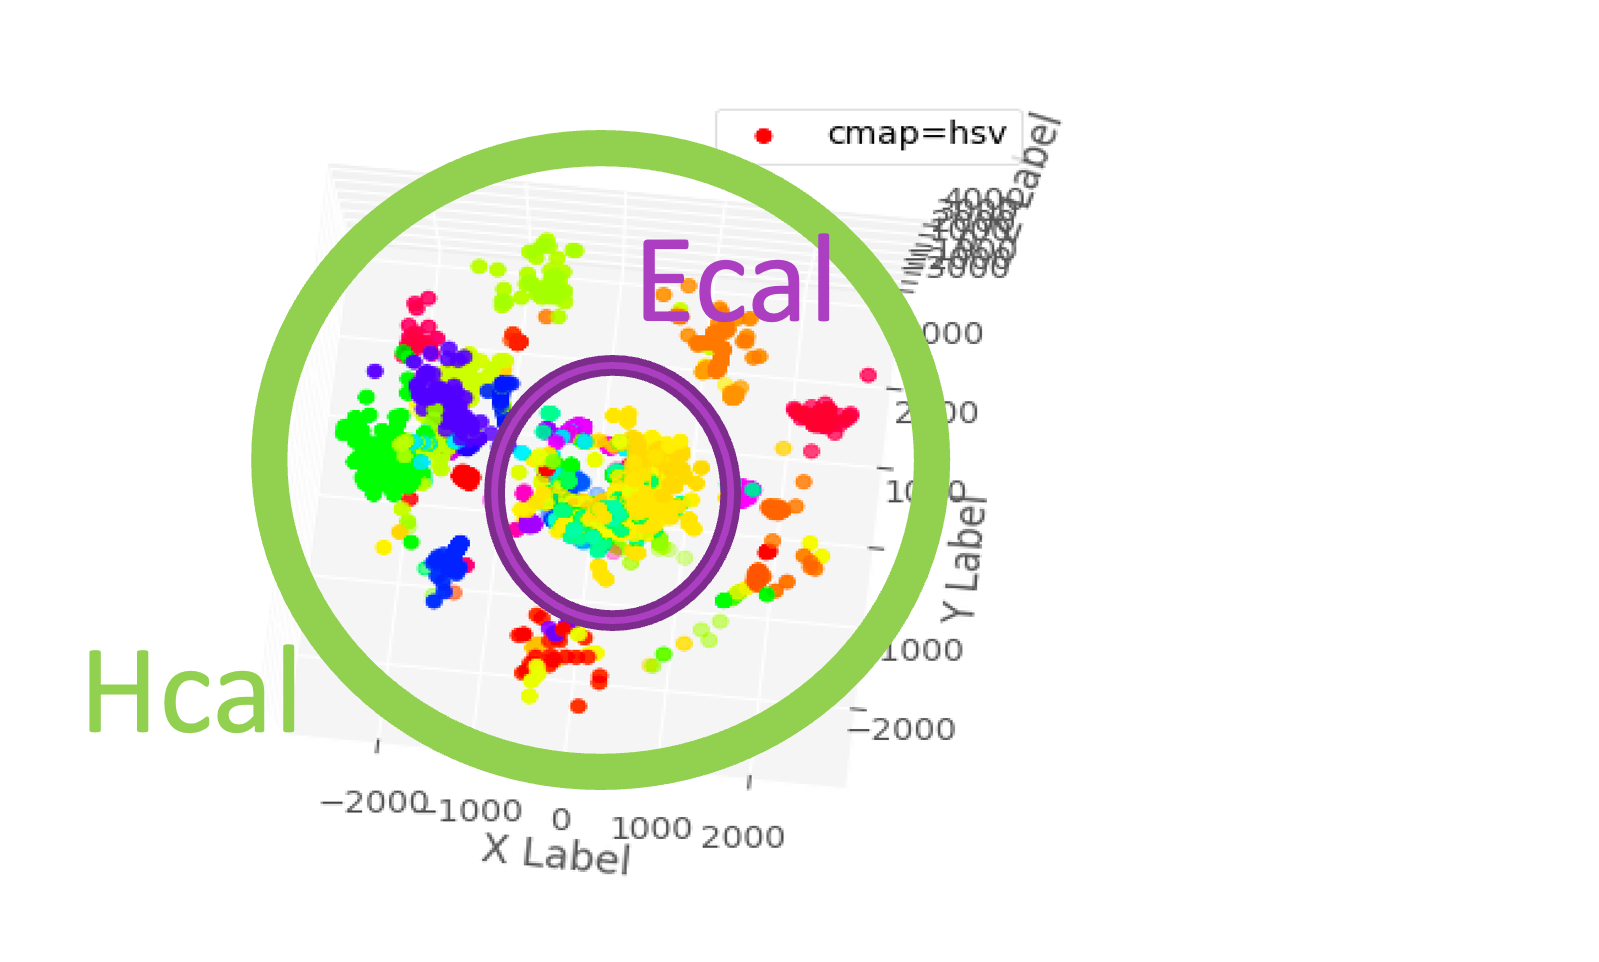
\includegraphics[width=250pt]{./Figure/DLAnalysis/Input2.png}%.5\linewidth]{./Figure/DLAnalysis/Input2.png}
			\caption{}
			\label{fig:sfig2}
		\end{center}
	\end{subfigure}
	\caption[入力データのヒット位置]{入力データのヒット位置の一例。(b)は(a)を上方向から見た図。EcalとHcalがそれぞれ含まれているのがわかる。}
	\label{Input}
\end{figure}

\begin{figure}[H]
	\begin{center}
		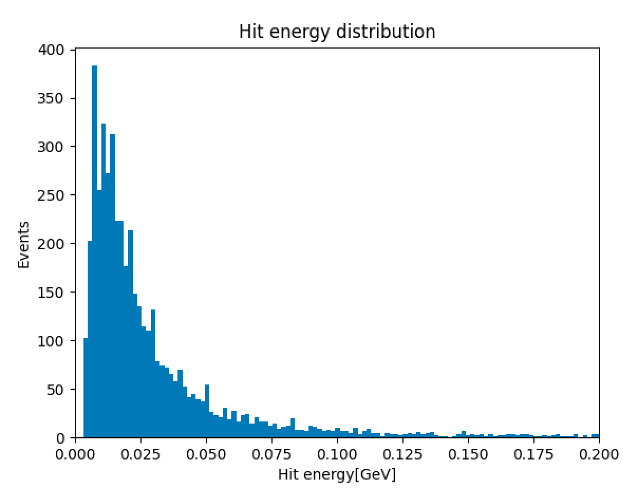
\includegraphics[width=250pt]{./Figure/DLAnalysis/Energydep.png}
		\caption[入力データのエネルギー損失]{シミュレーションデータのエネルギー損失の一例。}
		\label{EnergyDep}
	\end{center}
\end{figure}


入力データの事前処理として、パラメータの規格化をおこない、データ範囲が$[-1,1]$となるように調整した。ヒット位置はカロリメータの位置から$[-2000,2000]$の範囲に制限されているので、2000で除算をおこなった。一方、エネルギー損失については tanh関数で圧縮した。
以下にこれらのパラメータ整形をまとめる。

\begin{enumerate}
\item ヒットの位置
\[
(x',y',z') = \left(\frac{x}{2000},\frac{y}{2000},\frac{z}{2000}\right) 
\]
\item ヒットのエネルギー損失
\[
E' = \tanh(E)
\]
\end{enumerate}


\subsection{ネットワークの評価}
ネットワークの評価として、エポックに対する損失関数の変化と表現空間における1つのイベントのヒット分布を確認した。

訓練データおよび評価データの各エポックごとの損失関数は図\ref{Loss_ILD}のように推移した。

\begin{figure}[H]
	\begin{center}
		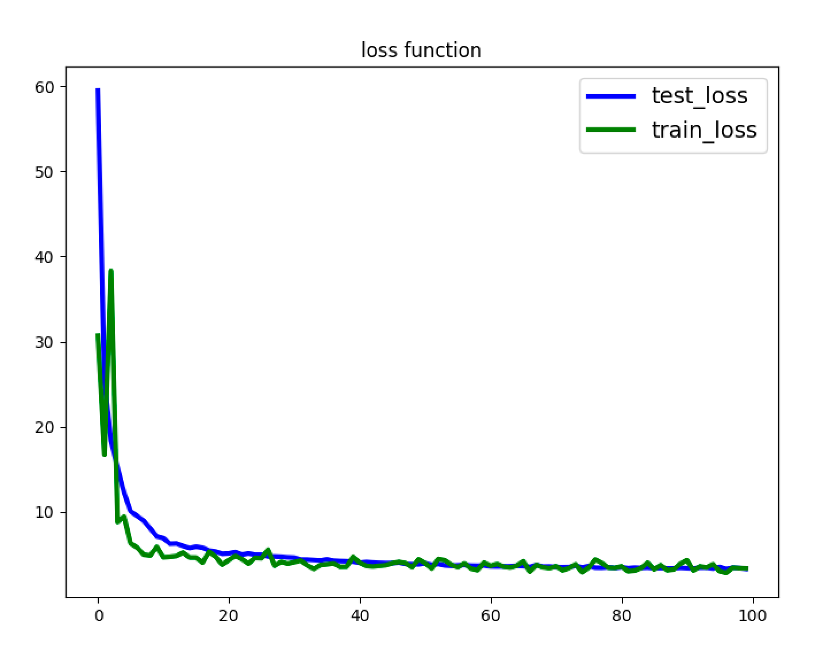
\includegraphics[width=250pt]{./Figure/DLAnalysis/Loss_ILD.png}
		\caption[損失関数の推移]{損失関数の推移。}
		\label{Loss_ILD}
	\end{center}
\end{figure}

どちらのデータも均等に損失関数が減少しており、適切に学習が行えていることがわかる。

また、ネットワークの評価として、Object Condensationから出力されたヒットの表現空間において、各クラスターが異なる位置に分類されているかどうかを確認した。学習前のプロットと30エポック学習後の表現空間が図\ref{representation}に示されている。

\begin{figure}[H]
	\begin{subfigure}{.5\textwidth}
		\begin{center}
 		 	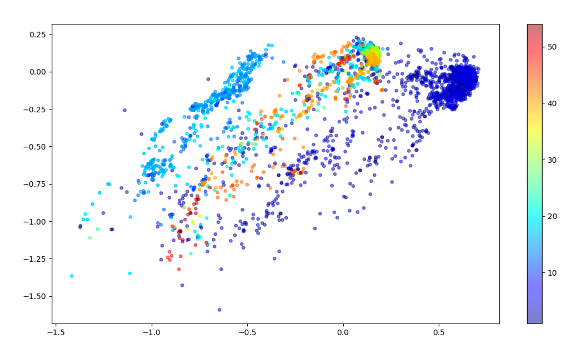
\includegraphics[width=200pt]{./Figure/DLAnalysis/Repre_before.png}%.5\linewidth]{./Figure/DLAnalysis/Input2.png}
  			\caption{}
  			\label{fig:sfig1}
 		\end{center}
	\end{subfigure}
	\begin{subfigure}{.5\textwidth}
		\begin{center}
			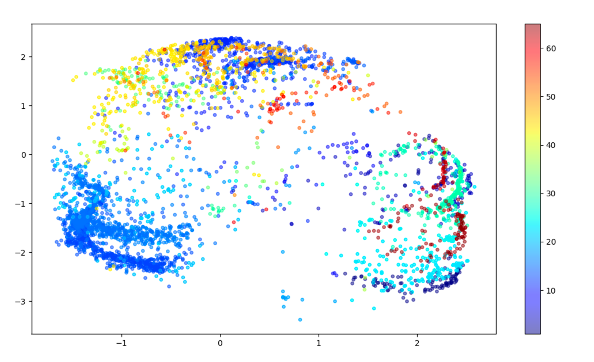
\includegraphics[width=200pt]{./Figure/DLAnalysis/Repre_30.png}%.5\linewidth]{./Figure/DLAnalysis/Input2.png}
			\caption{}
			\label{fig:sfig2}
		\end{center}
	\end{subfigure}
	\caption[学習前と30エポック学習後の表現空間の比較]{学習前と30エポック学習後の表現空間の比較。}
	\label{representation}
\end{figure}


それぞれの点がヒットを示しており、色がクラスター分けを示す。学習前のプロットにおいても学習後のプロットにおいても3つの分布に分かれていることが分かるが、学習後の方が表現空間におけるそれぞれのクラスター間の距離が大きくなっている。これは異なるクラスターを識別するためにそれぞれのクラスターに属するヒットの特徴量がネットワークにより学習されていることを示している。しかし表現空間における3つの分布の中に含まれるそれぞれのクラスターは十分に分けられていない。


\section{2光子事象を用いたカロリメトリー}
%%%%%%%%%%%%%%%%%%%%%%%%%%%%%%%%%%%%%%%%%%%%%%%%%%%%%%%%%%%%%%%%%%%%%%%%%%%%%%%%%%%%%%%%%%%%%
\end{comment}
\subsection{入力データ}
入力データとして、近接する2光子イベントの検出器シミュレーションデータを作成した。ビーム衝突点から特定の角度で2本の光子を入射させ、極角を$\SI{85}{rad}$に固定し方位角$\phi$をランダムに取ることで訓練用及び評価用のデータを作成した。角度は$\SI{1/10}{ rad}$の識別のより困難なケースから$\SI{5/10}{ rad}$のより容易なケースまで、$\SI{0.1}{rad}$ずつ、5つのファイルをそれぞれ20000イベント用意した。光子の運動量は$\SI{5}{GeV}$、検出器シミュレーションにより出力されるのは各ヒットの位置、エネルギー損失やその生成元となるモンテカルロシミュレーション(Monte Carlo simulation, MC)粒子の情報を持ったLCIOファイルである。LCIOファイルはPythonによって読み込みが可能であるが、深層学習を適用するためにはデータの選定と事前処理が必要である。データを読み込む際に毎回この処理を行うと時間がかかりすぎるので、このファイルをPythonコードにより変換し、各イベントごとに深層学習に適したフォーマットであるnpzファイルを作成した。npzファイルにはヒットの情報として位置($x$,$y$,$z$)および各エネルギー損失が含まれる。ヒットの時間情報は今回は使用しなかった。正解ラベルとして、各ヒットが生成されたMC粒子のIDをもとにした番号を割り当てた。番号はMC粒子の種類に関わらず、0から昇順に生成された。

図\ref{DoublePG}にこのデータの概形を示す。

\begin{figure}[H]
	\begin{subfigure}{.5\textwidth}
		\begin{center}
 		 	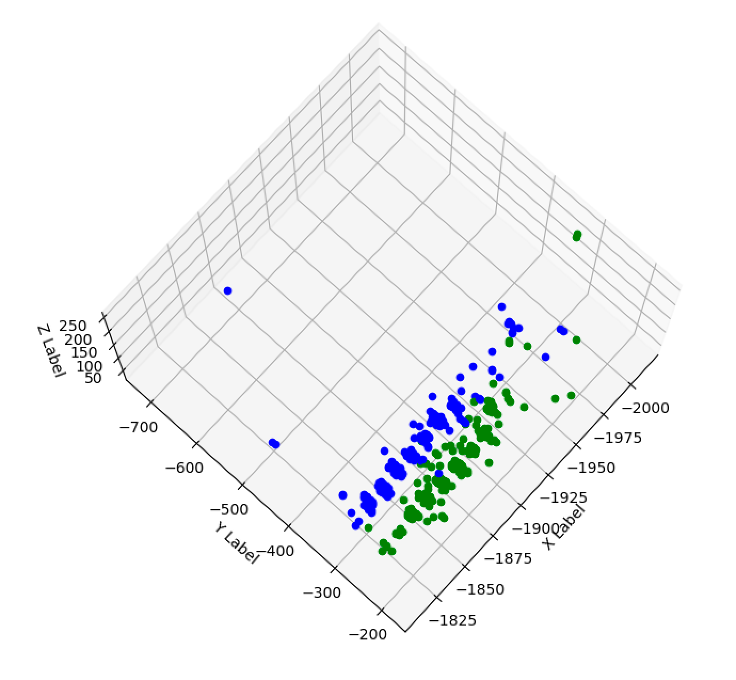
\includegraphics[width=200pt]{./Figure/DLAnalysis/Double1.png}%.5\linewidth]{./Figure/DLAnalysis/Input2.png}
  			\caption{}
  			\label{fig:sfig1}
 		\end{center}
	\end{subfigure}
	\begin{subfigure}{.5\textwidth}
		\begin{center}
			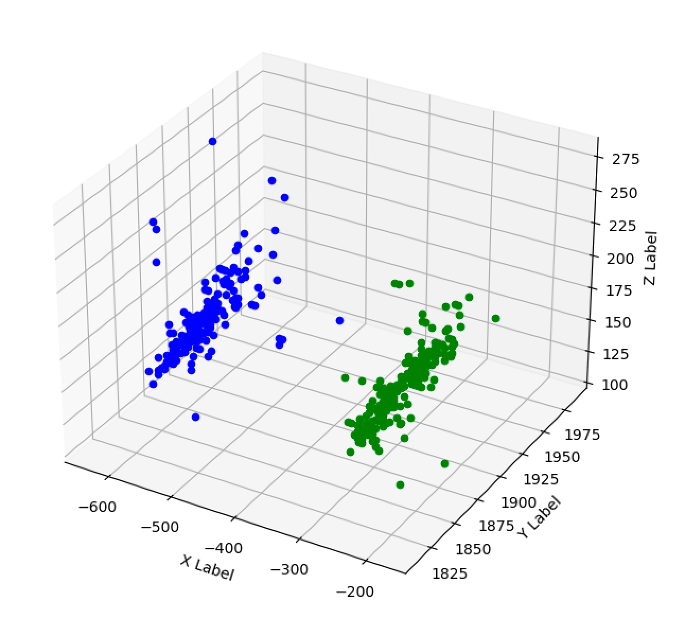
\includegraphics[width=200pt]{./Figure/DLAnalysis/Double5.png}%.5\linewidth]{./Figure/DLAnalysis/Input2.png}
			\caption{}
			\label{fig:sfig2}
		\end{center}
	\end{subfigure}
	\caption[DoubleParticleGunによる$\SI{0.5}{rad}$および$\SI{0.1}{rad}$の場合の入力データのヒット位置]{$\SI{0.5}{rad}$および$\SI{0.1}{rad}$の場合の入力データのヒット位置。}
	\label{DoublePG}
\end{figure}

入力データの事前処理として、パラメータの規格化をおこない、データ範囲が$[-1,1]$となるように調整した。ヒット位置はカロリメータの位置から$[-2000,2000]$の範囲に制限されているので、2000で除算をおこなった。一方、エネルギー損失については tanh関数で圧縮した。
以下にこれらのパラメータ整形をまとめる。

\begin{enumerate}
\item ヒットの位置
\[
(x',y',z') = \left(\frac{x}{2000},\frac{y}{2000},\frac{z}{2000}\right) 
\]
\item ヒットのエネルギー損失
\[
E' = \tanh(E)
\]
\end{enumerate}
訓練用データとして、全データの80\%にあたる80000イベントを用い、評価用データとして残りの20000イベントを使用した。学習は各角度で行い、同じ角度で推論を行った。

\subsection{ネットワークの評価}
ネットワークの評価として、Object Condensationから出力された$\beta_i$をもとに各々のヒットをクラスター分けし、それらを3Dプロット上で正解ラベルと比較した。

図\ref{DoublePG_5_res}は2光子の角度が$\SI{0.5}{rad}$の場合のプロットである。図(a)は良くクラスタリングできている例を示している。一方、図(b)は一つのヒットが異なって識別されているものを示した。図(b)から、二つのクラスターの境界付近において識別がやや困難になっている可能性がある。

\begin{figure}[H]
	\begin{subfigure}{.5\textwidth}
		\begin{center}
 		 	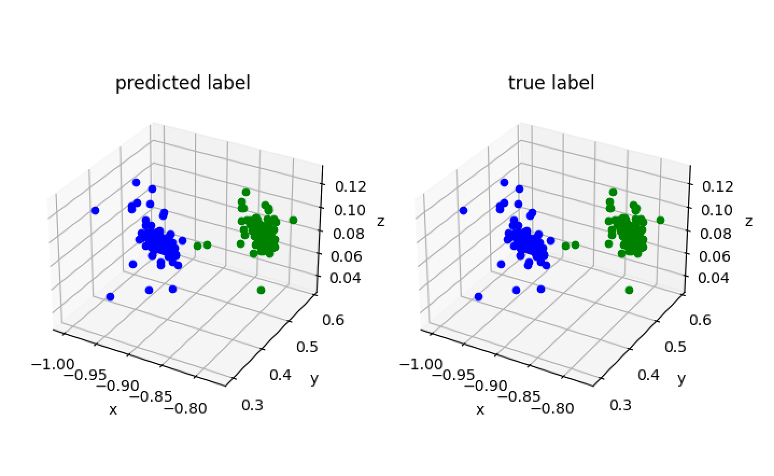
\includegraphics[width=200pt]{./Figure/DLAnalysis/Double5_1.png}%.5\linewidth]{./Figure/DLAnalysis/Input2.png}
  			\caption{}
  			\label{DPG_res_a}
 		\end{center}
	\end{subfigure}
	\begin{subfigure}{.5\textwidth}
		\begin{center}
			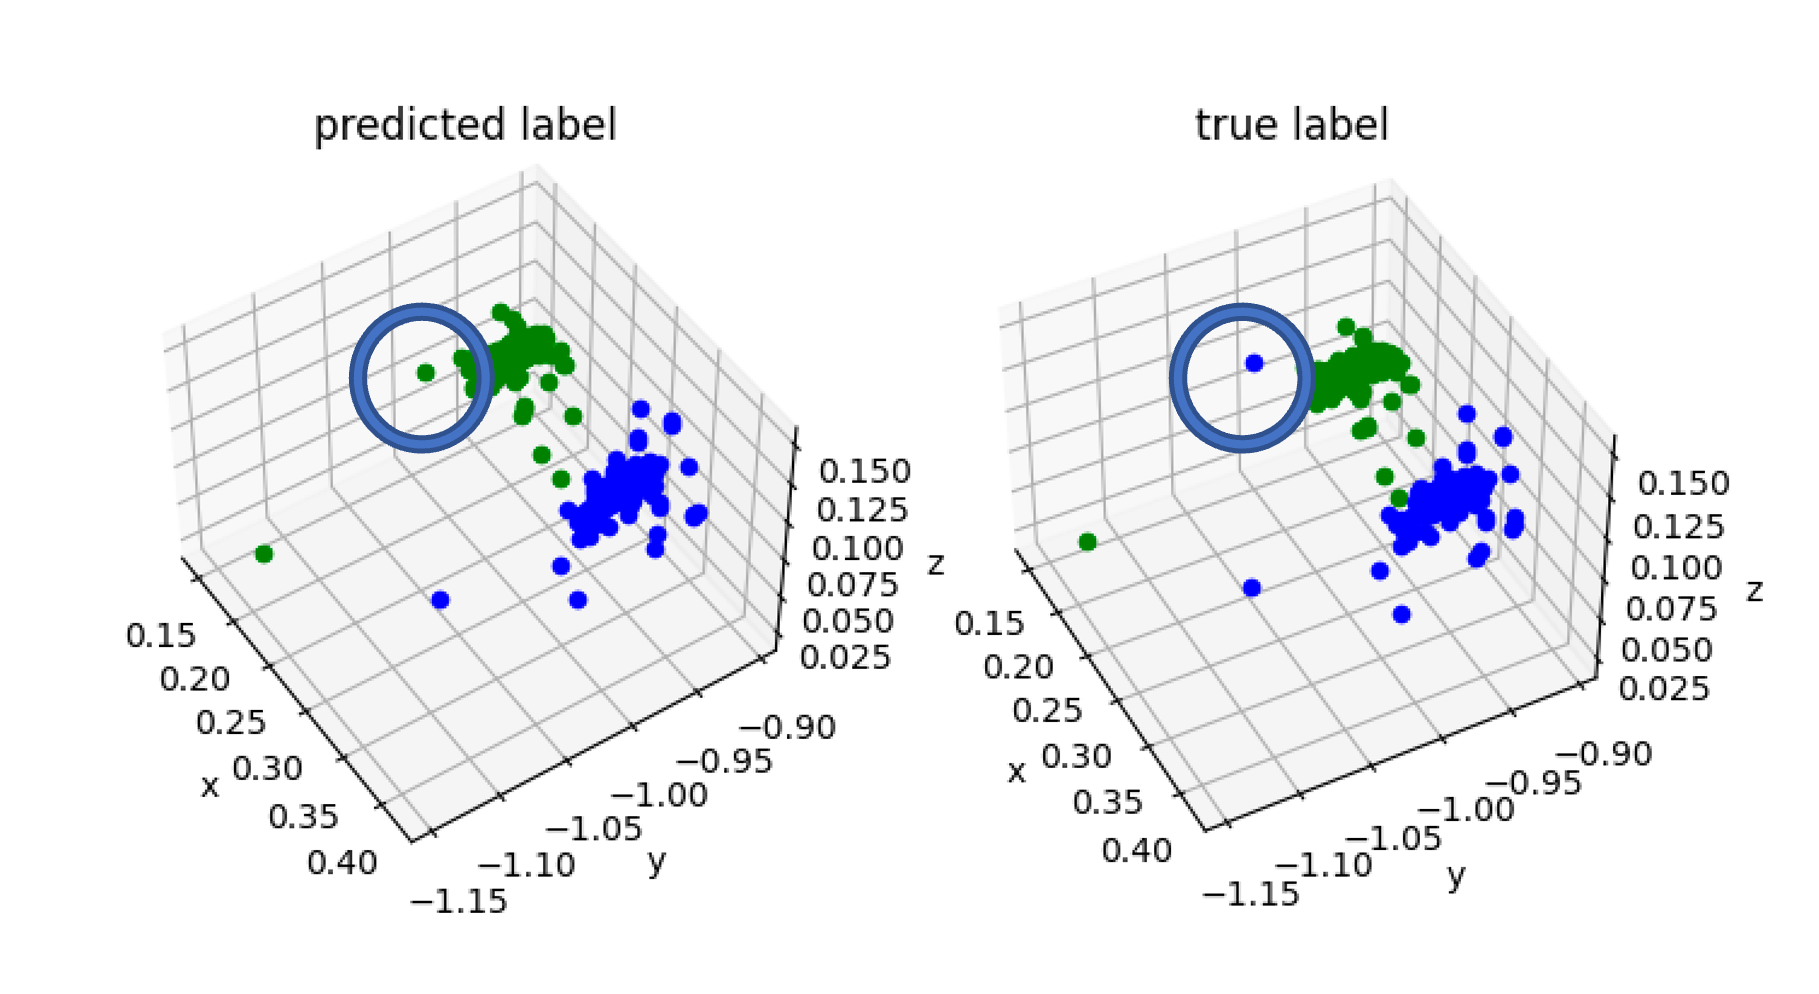
\includegraphics[width=200pt]{./Figure/DLAnalysis/Double5_2.png}%.5\linewidth]{./Figure/DLAnalysis/Input2.png}
			\caption{}
			\label{DPG_res_b}
		\end{center}
	\end{subfigure}
	\caption[$\SI{0.5}{rad}$の場合の比較]{$\SI{0.5}{rad}$の場合のネットワークにより予測されたラベルと正解ラベルの比較。(a)は全てのヒットが正しく識別できている場合。(b)は一つのヒットが誤って識別されている場合。}
	\label{DoublePG_5_res}
\end{figure}

図\ref{DoublePG_1_res}は2光子の角度が$\SI{0.1}{rad}$の場合の場合のプロットである。先ほどとは異なり、多くのイベントは図のように3つにクラスタリングされており、先ほどのケースよりも識別が難しいことを確認した。
\begin{figure}[H]
	\begin{subfigure}{.5\textwidth}
		\begin{center}
 		 	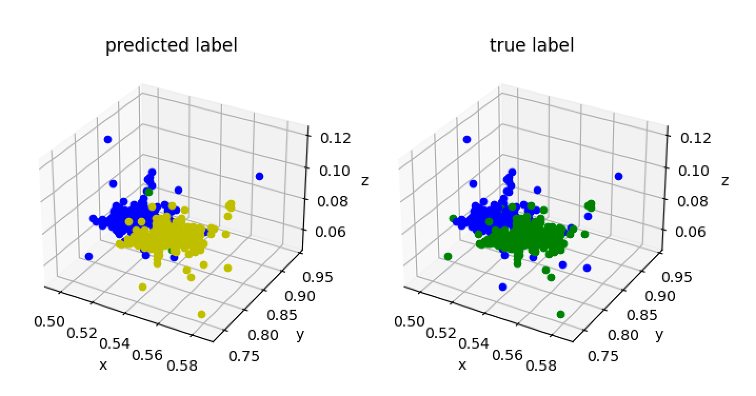
\includegraphics[width=200pt]{./Figure/DLAnalysis/Double1_2.png}%.5\linewidth]{./Figure/DLAnalysis/Input2.png}
  			\caption{}
  			\label{DPG_res_a}
 		\end{center}
	\end{subfigure}
	\begin{subfigure}{.5\textwidth}
		\begin{center}
			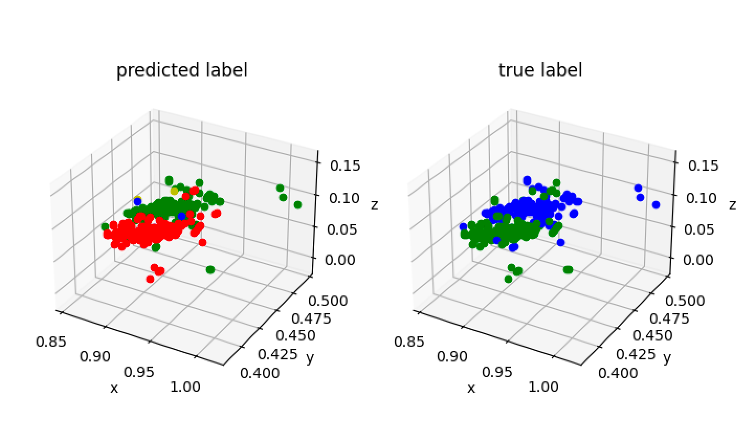
\includegraphics[width=200pt]{./Figure/DLAnalysis/Double1_1.png}%.5\linewidth]{./Figure/DLAnalysis/Input2.png}
			\caption{}
			\label{DPG_res_b}
		\end{center}
	\end{subfigure}
	\caption[$\SI{0.5}{rad}$の場合の場合の比較]{$\SI{0.5}{rad}$の場合のネットワークにより予測されたラベルと正解ラベルの比較。(a)、(b)ともにいくつかのヒットが誤って識別されている。}
	\label{DoublePG_1_res}
\end{figure}

これらのイベントの中には光子が変換して他のMC粒子が生成されているものもあったが、それらについては正解ラベルの数が3以上のものを基準として除外している。

次に、定量的にクラスタリングの精度を以下の式で定義し、比較を行った。
\begin{equation}
\textrm{accuracy} = \frac{\textrm{predicted\ hit\ with\ correct\ label}}{\textrm{true\ label}}
\end{equation}

5つのシミュレーションデータに対して、イベントに含まれるクラスターごとに上記の値を計算し、全イベントにわたってプロットしたものを図\ref{result_DoublePG}に示す。

\begin{figure}[H]
	\begin{subfigure}{.5\textwidth}
		\begin{center}
 		 	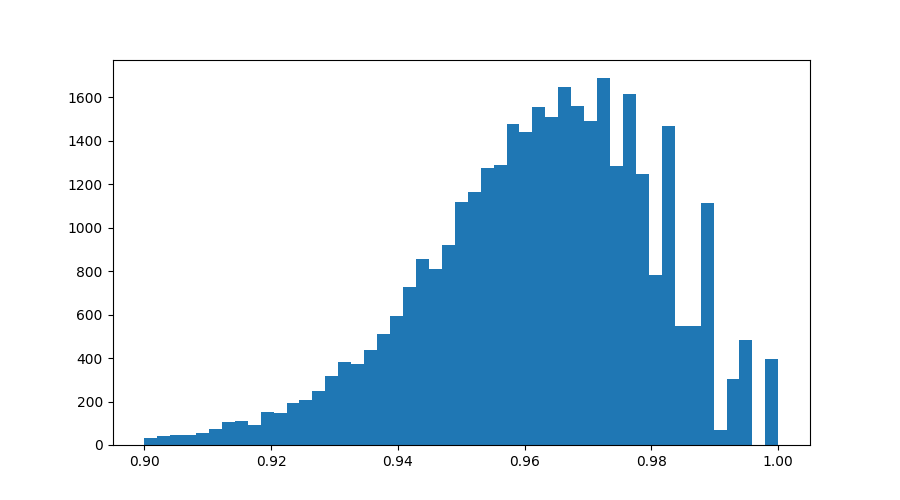
\includegraphics[width=200pt]{./Figure/DLAnalysis/rate_pred_1.png}%.5\linewidth]{./Figure/DLAnalysis/Input2.png}
  			\caption{$\SI{0.1}{rad}$}
  			\label{fig:sfig1}
 		\end{center}
	\end{subfigure}
	\begin{subfigure}{.5\textwidth}
		\begin{center}
			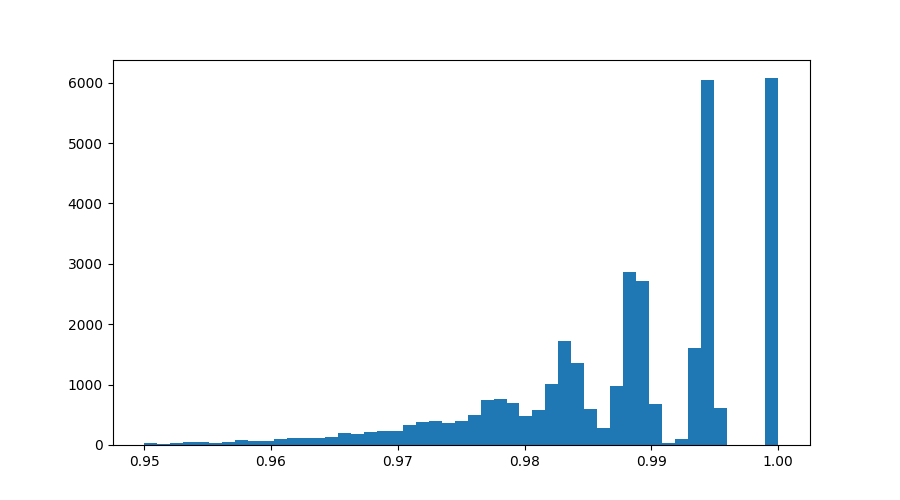
\includegraphics[width=200pt]{./Figure/DLAnalysis/rate_pred_2.png}%.5\linewidth]{./Figure/DLAnalysis/Input2.png}
			\caption{$\SI{0.2}{rad}$}
			\label{fig:sfig2}
		\end{center}
	\end{subfigure}
		\begin{subfigure}{.5\textwidth}
		\begin{center}
			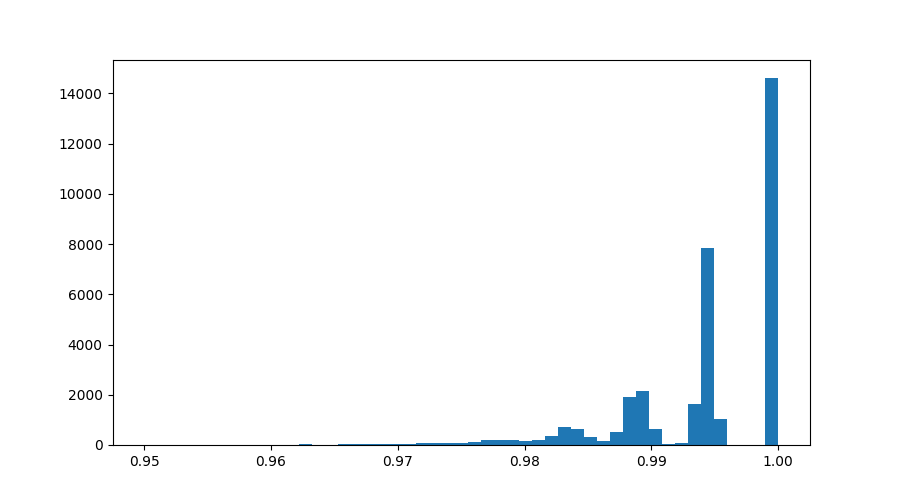
\includegraphics[width=200pt]{./Figure/DLAnalysis/rate_pred_3.png}%.5\linewidth]{./Figure/DLAnalysis/Input2.png}
			\caption{$\SI{0.3}{rad}$}
			\label{fig:sfig2}
		\end{center}
	\end{subfigure}
		\begin{subfigure}{.5\textwidth}
		\begin{center}
			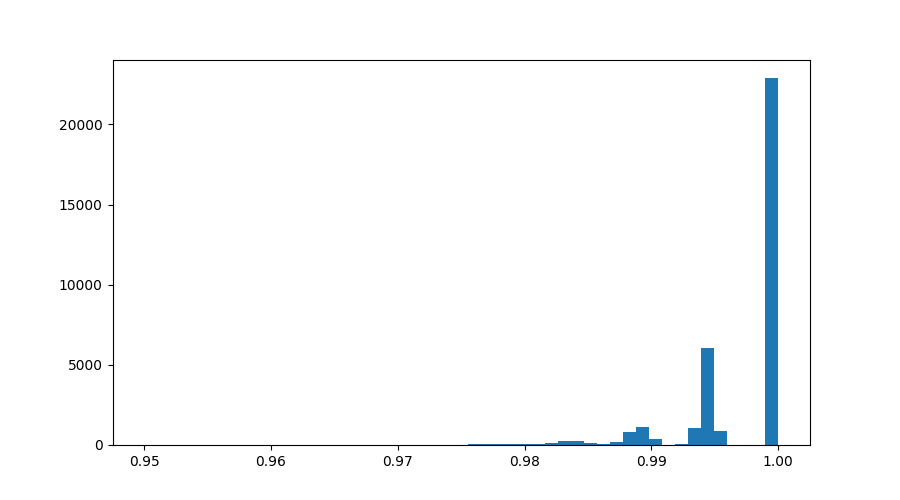
\includegraphics[width=200pt]{./Figure/DLAnalysis/rate_pred_4.png}%.5\linewidth]{./Figure/DLAnalysis/Input2.png}
			\caption{$\SI{0.4}{rad}$}
			\label{fig:sfig2}
		\end{center}
	\end{subfigure}
	\begin{subfigure}{.5\textwidth}
		\begin{center}
			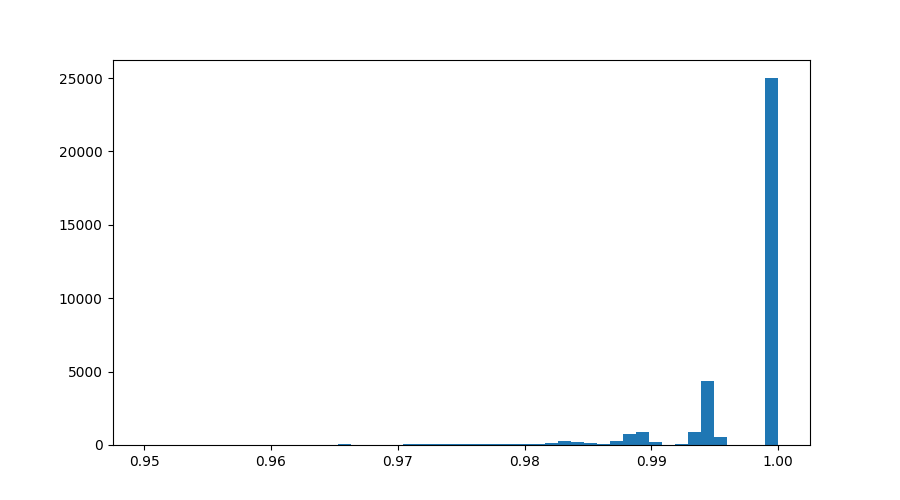
\includegraphics[width=200pt]{./Figure/DLAnalysis/rate_pred_5.png}%.5\linewidth]{./Figure/DLAnalysis/Input2.png}
			\caption{$\SI{0.5}{rad}$}
			\label{fig:sfig2}
		\end{center}
	\end{subfigure}

	\caption[2光子事象による$\SI{0.1}{rad}$から$\SI{0.5}{rad}$までのシミュレーションデータの各クラスターごとの正しく識別できたヒット数]{2光子事象による$\SI{0.1}{rad}$から$\SI{0.5}{rad}$までのシミュレーションデータの各クラスターごとの正しく識別できたヒット数。横軸はaccuracy、縦軸はクラスター数を表す。}
	\label{result_DoublePG}
\end{figure}

%%%%%%%%%%%%%%%%%%%%%%%%%%%%%%%%%%%%%%%%%%%%%%%%%%%%%%%%%%%%%%%%%%%%%%
\begin{comment}
\begin{figure}[H]
	\begin{center}
		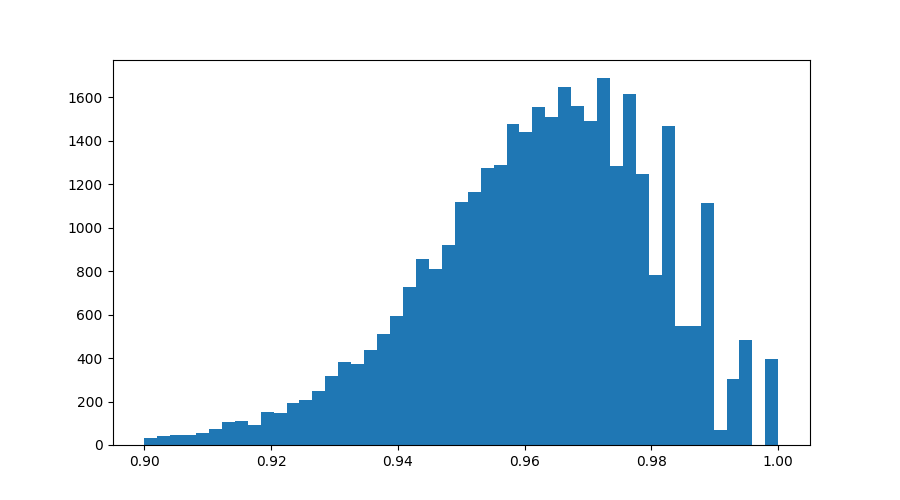
\includegraphics[width=250pt]{./Figure/DLAnalysis/rate_pred_1.png}
		\caption[角度$\SI{0.1}{rad}$のシミュレーションデータの各クラスターごとの正しく識別できたヒット数]{角度$\SI{0.1}{rad}$のシミュレーションデータの各クラスターごとの正しく識別できたヒット数。横軸は縦軸がクラスターの数}
		\label{result_DoublePG1}
	\end{center}
\end{figure}

\begin{figure}[H]
	\begin{center}
		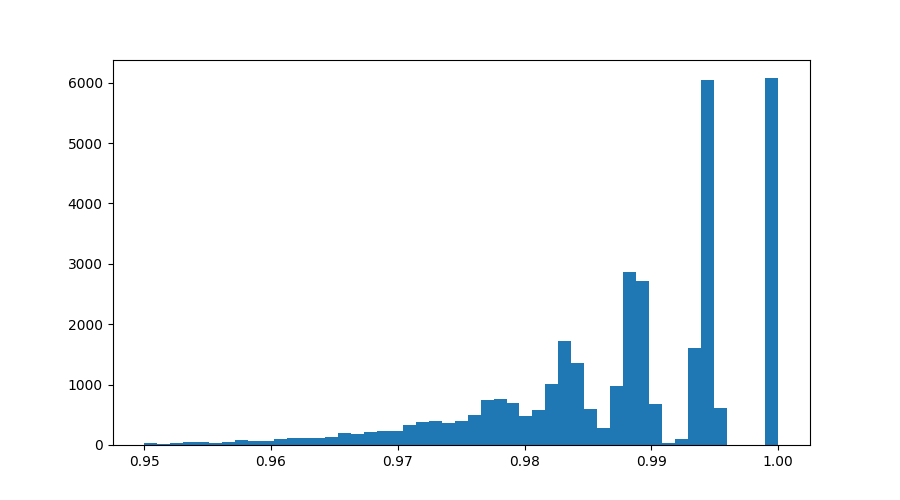
\includegraphics[width=250pt]{./Figure/DLAnalysis/rate_pred_2.png}
		\caption[角度$\SI{0.2}{rad}$のシミュレーションデータの各クラスターごとの正しく識別できたヒット数]{角度$\SI{0.2}{rad}$のシミュレーションデータの各クラスターごとの正しく識別できたヒット数。}
		\label{result_DoublePG2}
	\end{center}
\end{figure}

\begin{figure}[H]
	\begin{center}
		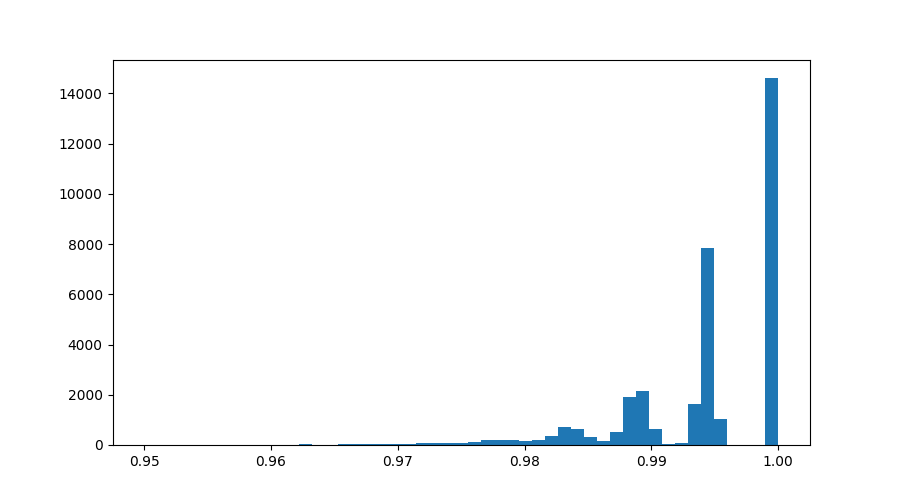
\includegraphics[width=250pt]{./Figure/DLAnalysis/rate_pred_3.png}
		\caption[角度$\SI{0.3}{rad}$のシミュレーションデータの各クラスターごとの正しく識別できたヒット数]{角度$\SI{0.3}{rad}$のシミュレーションデータの各クラスターごとの正しく識別できたヒット数。}
		\label{result_DoublePG3}
	\end{center}
\end{figure}

\begin{figure}[H]
	\begin{center}
		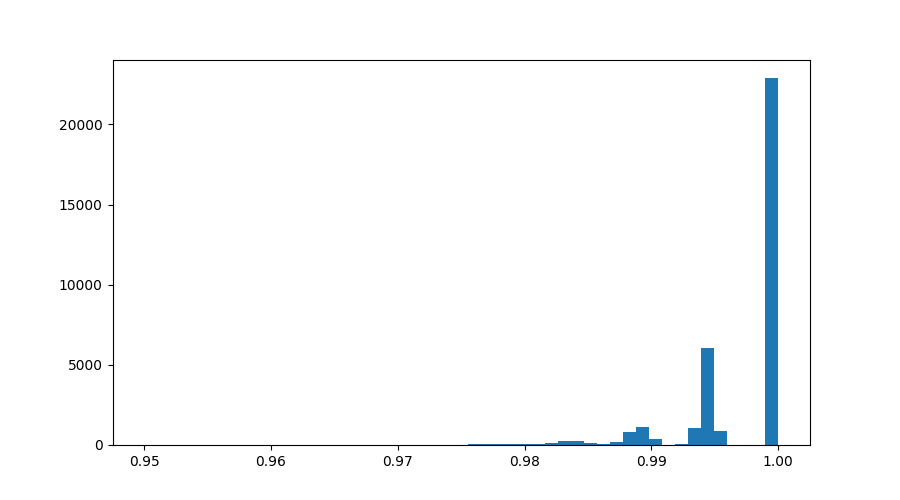
\includegraphics[width=250pt]{./Figure/DLAnalysis/rate_pred_4.png}
		\caption[角度$\SI{0.4}{rad}$のシミュレーションデータの各クラスターごとの正しく識別できたヒット数]{角度$\SI{0.4}{rad}$のシミュレーションデータの各クラスターごとの正しく識別できたヒット数。}
		\label{result_DoublePG4}
	\end{center}
\end{figure}

\begin{figure}[H]
	\begin{center}
		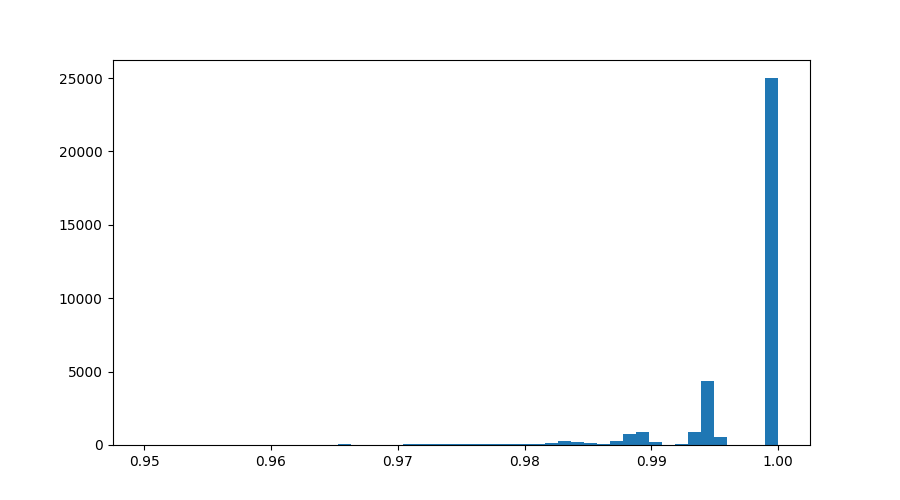
\includegraphics[width=250pt]{./Figure/DLAnalysis/rate_pred_5.png}
		\caption[角度$\SI{0.5}{rad}$のシミュレーションデータの各クラスターごとの正しく識別できたヒット数]{角度$\SI{0.5}{rad}$のシミュレーションデータの各クラスターごとの正しく識別できたヒット数。}
		\label{result_DoublePG5}
	\end{center}
\end{figure}
\end{comment}
%%%%%%%%%%%%%%%%%%%%%%%%%%%%%%%%%%%%%%%%%%%%%%%%%%%%%%%%%%%%%%%%%%%%%%%%%%%%%%%%%


各イベントごとに測定された、各クラスターの精度の平均値を表\ref{acc_Grav}にまとめる。

\begin{table}[h]
	\begin{center}
		\begin{tabular}{|c|c|c|c|c|c|}
		\hline
		角度$[\SI{}{rad}]$&0.1&0.2&0.3&0.4&0.5\\\hline\hline
		accuracy[\%]&96.08&98.64&99.30&99.68&99.56\\\hline
		\end{tabular}
	\end{center}
	\caption[角度ごとの各クラスターの精度の平均値]{角度ごとの各クラスターの精度の平均値。}
\label{acc_Grav}
\end{table}

$\SI{0.5}{rad}$のデータは99.56\%の精度を達成しているが、角度が小さくなるにつれ精度は悪化し、$\SI{0.1}{rad}$の時点では96.08\%まで減少している。これはシャワーの重なりが大きくなったことで識別が難しくなっているために生じていると考えられる。また、各ヒストグラムについて分布に離散的な飛びが生じているのが確認できる。これはそれぞれの山ごとに誤ってラベルが付けられたヒットの数が1個、2個、$\cdots$と対応していることが考えられる。さらに、本来識別が容易な$\SI{0.5}{rad}$のクラスターよりも$\SI{0.4}{rad}$の方が精度が高くなっている。それぞれのヒストグラムを見ると、(d)に含まれるピークは(e)に含まれるピークよりも全体的に少なくなっているように見える。このことから、原因としてはデータの揺らぎによる影響だけでなく、$\SI{0.4}{rad}$のイベントの中に光子が変換されて生じた正解ラベルクラスターの数が3以上のものが多く含まれているために、全体のイベント数に偏りが生じているためではないかと考えた。これを確かめるためには実際にカットされなかったイベント数を数える必要がある。

さらに、今回は2つの光子のみの単純なデータであったが、実際のILDへ適用するにあたり、さらに複雑なシミュレーションデータを用意し、性能評価および最適化をする必要があると考える。


%およそ70\%のクラスターに含まれるヒットが正しくラベルを識別できていることがわかる。
%残りの30\%のクラスターについて、なぜラベルを識別できていないか確認するために一つのイベントについて図のように3Dプロットで確認した。

%本手法は後述するEBES実験における2光子検出に対しても有効であり、本研究はその応用に向けた初期研究である。

 % !TEX root = ../MasterThesis.tex

\chapter{EBES実験におけるバックグラウンド測定} \label{sec:EBES}
未確認粒子であるALPsの探索を目的としたEBES実験を行うにあたって、バックグラウンド測定を実施した。本章ではその概要と結果を報告する。

5.1節では実験に使用するビームラインKEK Linacについて述べる。5.2節では実験本番に予定している実験セットアップを説明する。5.3節では2022年7月に行ったバックグラウンド測定の概要とその結果を示す。
%\section{実験本番のセットアップ}

\section{KEK Linac}
本実験はKEKにあるLinacの第3スイッチヤードにおいて実験を予定している。
%%%%%%%%%%%%%%%%%%%%%%%%%%%%%%%%%%%%%%%%%%%%%
\begin{comment}
LinacはSuperKEKBの前段加速器であり、その概形を図\ref{SuperKEKB}に示す。
\begin{figure}[H]
	\begin{center}
		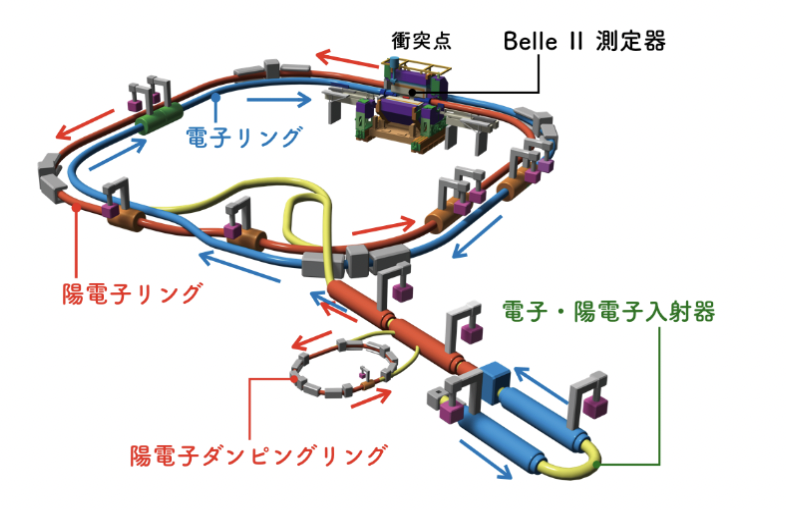
\includegraphics[width=250pt]{./Figure/EBES/SuperKEKB.png}
		\caption[SuperKEKB加速器]{SuperKEKB加速器。}
		\label{SuperKEKB}
	\end{center}
\end{figure}
\end{comment}
%%%%%%%%%%%%%%%%%%%%%%%%%%%%%%%%%%%%%%%%%%%%%
本ビームラインでは、エネルギーが最大$\SI{7}{GeV}$の電子ビームおよび$\SI{4}{GeV}$の陽電子ビームが利用可能である。%Super KEKBは設計ルミノシティ$8\times 10^{35}\SI{}{cm^{-2}s^{-1}}$の電子・陽電子加速器であり、ビームメインラインの周長はおよそ$\SI{3}{km}$である。
%ビームは電子・陽電子入射器で生成された後、それぞれのダンピングリングを通じてメインラインを周回する。

第3スイッチヤードはLinacビームライン終端に位置しており、この概形を図\ref{SY3}に示す。
\begin{figure}[H]
	\begin{center}
		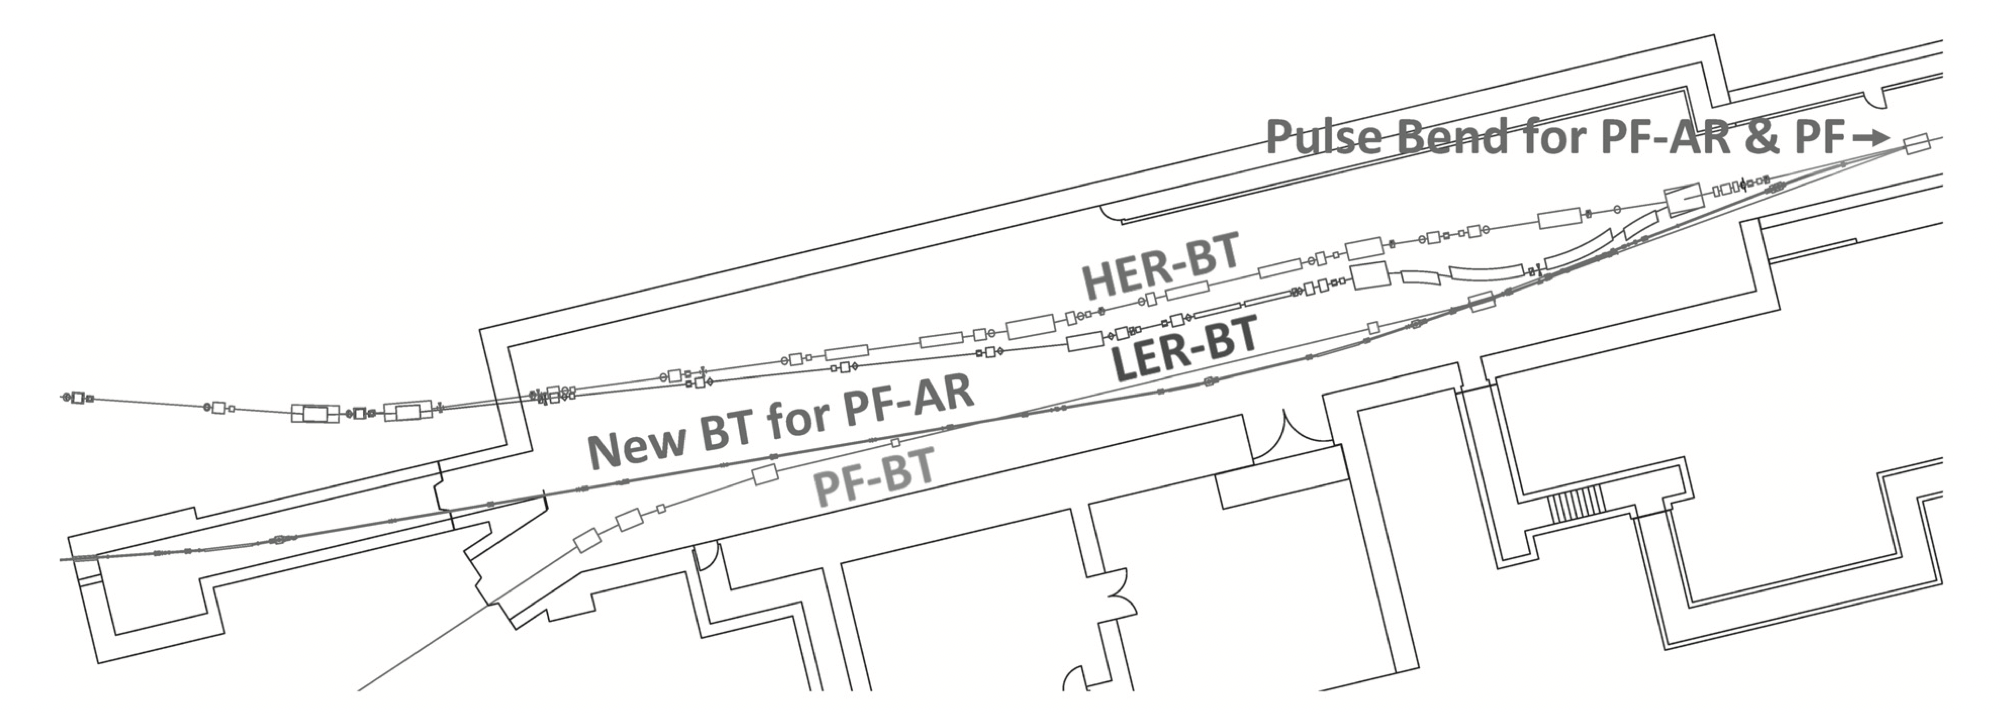
\includegraphics[width=250pt]{./Figure/EBES/SY3.png}
		\caption[第3スイッチヤード]{第3スイッチヤード。}
		\label{SY3}
	\end{center}
\end{figure}

第3スイッチヤード入口と第3スイッチヤードにはPF/PF-AR用のビーム輸送路へビームを選択的に導くパルス偏向電磁石とSuperKEKB HER/LER に入射する電子、陽電子ビームを分離する偏向電磁石とビームダンプにビームを導くための偏向電磁石が設置してある。第3スイッチヤード入口まで輸送されてきたビームはビームの輸送先に応じてパルス偏向電磁石と偏向電磁石の電流値が設定される。ビームダンプは SuperKEKB HER 用のビームラインから分岐したビームラインのため、SY3ビームダンプを使った実験はビームダンプ専用の運転に切り替えて行う。
SY3で実験を行う長所として、高いエネルギー(最大7 GeV)と高いビーム繰り返し(最大50 Hz)、可変なバンチチャージ(最大 4 nC)が挙げられる。高いエネルギーによりALPsが相対論的にブーストされ、寿命を伸ばすことができる。また、高ビーム繰り返しにより高い統計量を得ることができるため、小さい結合定数であったとしても探索に貢献できる可能性が高まる。そして、バンチチャージを変更することでバックグラウンドの割合をコントロールできる。

\section{実験セットアップ}
本実験において重要となるのがミューオンや中性子などによって生じるバックグラウンドであり、実験セットアップには十分バックグラウンドイベントを低減できるような工夫が必要となる。本実験で予定している検出器セットアップは2種類あり、それぞれセットアップ1、セットアップ2と呼ぶ。その模式図を図\ref{EBES_1}、\ref{EBES_2}に示す。
\begin{figure}[H]
	\begin{center}
		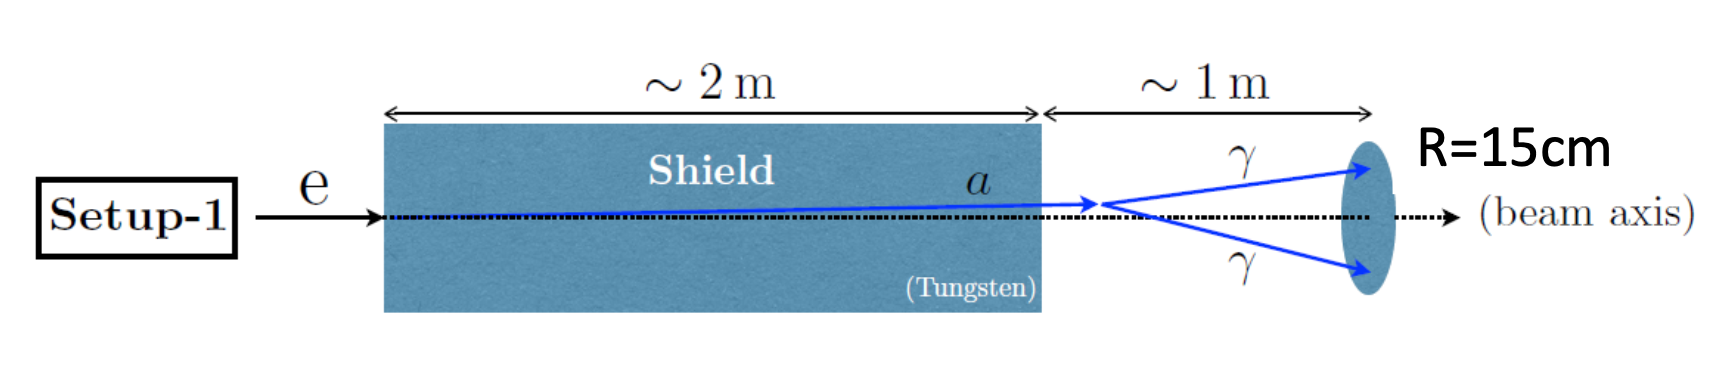
\includegraphics[width=270pt]{./Figure/EBES/EBES_1.png}
		\caption[EBES実験セットアップ1]{EBES実験セットアップ1。}
		\label{EBES_1}
	\end{center}
\end{figure}

\begin{figure}[H]
	\begin{center}
		\includegraphics[width=330pt]{./Figure/EBES/EBES_2.png}
		\caption[EBES実験セットアップ2]{EBES実験セットアップ2。一部のシールドを除去し、磁場を印加している。}
		\label{EBES_2}
	\end{center}
\end{figure}


図\ref{EBES_1}にセットアップ1の模式図を示す。バックグラウンド除去のためにビームダンプ全体をタングステンシールドで遮蔽する。ビームダンプから\SI{1}{m}ほどの距離に置いた検出器で2光子事象を観測する。

図\ref{EBES_2}に示したのがセットアップ2である。シールドを一部除去し、ミューオンを偏極電磁石によって掃引する。
今回目的とするような結合定数の小さい反応をとらえる上でできるかぎりバックグラウンドイベントを低減させることが重要となる。


\section{バックグラウンド測定}
本実験を行う準備として、同じビームラインにおいてテストビームを用いた最初のバックグラウンド測定を行った。5.2.1節では、そのセットアップについて、5.2.2節ではその結果について説明する。

\subsection{バックグラウンド測定のためのセットアップ}
本実験は2022年7月11日から12日まで行われた。%ビームラインの軸上にビームダンプを設置し、図\ref{EBES_det}のように鉛ガラス検出器を設置した。
ステージを2つ用意し、それぞれビームダンプステージおよび検出器ステージとして利用した。ビームダンプとして鉛および鉄を設置し、その上部に鉛ガラス検出器を配置した。検出器ステージの上にはSiW ECALレイヤーを1台設置し、その後ろに鉛ガラス検出器を5台設置した。SiW ECALは本実験においてバックグラウンド削減のために使用されるが、今回の測定ではタングステンを設置していないため荷電粒子の識別を意図して設置した。

\begin{figure}[H]
	\begin{center}
		\includegraphics[width=330pt]{./Figure/EBES/EBES_det.pdf}
		\caption[バックグラウンド測定のためのセットアップ]{バックグラウンド測定のためのセットアップ。LGが鉛ガラス検出器、SiがSiW ECALレイヤー、Pb、Steelはそれぞれ遮蔽のための鉛および鉄ブロック、Stageはステージである。}
		\label{EBES_det}
	\end{center}
\end{figure}


鉛ガラス検出器およびSiW ECALにより生じた信号は、別室に接続されたPCへとデータが送信される。鉛ガラス検出器にはNIMモジュールを用いた論理回路を作成し、CAMAC PCによるデータ記録を行った。SiW ECALについてはSLボードに接続されたUSBケーブルによって直接PCへとデータが送信される。

電子および陽電子ビームの輸送は図\ref{EBES_beam1}および\ref{EBES_beam2}のように行われる。図(a)と図(b)は接続しており、両方の図に含まれる四極DC電磁石QF61A1は同じものである。偏向電磁石で軌道を曲げられたビームは四重極電磁石によって収束された後、再度偏向電磁石に曲げられビームダンプへと衝突する。

\begin{figure}[H]
		%\begin{center}
 		 	\includegraphics[width=400pt]{./Figure/EBES/EBES_beam1.png}%.5\linewidth]{./Figure/DLAnalysis/Input2.png}
 		%\end{center}
	\caption[加速器セットアップの模式図]{加速器セットアップの模式図。}
	\label{EBES_beam1}
\end{figure}

\begin{figure}[H]
		%\begin{center}
 		 	\includegraphics[width=400pt]{./Figure/EBES/EBES_beam2.png}%.5\linewidth]{./Figure/DLAnalysis/Input2.png}
   		%\end{center}
	\caption[加速器セットアップの模式図2]{加速器セットアップの模式図2。}
	\label{EBES_beam2}
\end{figure}



ビーム生成方法として、RF(radio frequency, 高周波)および熱電子銃を使用し、ビームの種類やビーム繰り返し、ビームエネルギーを変化させて検出器応答を確認した。表\ref{EBES_run}は長時間データを記録できた主な測定時間を示している。鉛ガラス検出器に印加する電圧やCAMACチャンネルとの対応は適宜変更されている。

%$測定時間[\SI{}{min} : 表に追加しようと思ったがランリストに一部記録していなかったのでやめた

\begin{table}[h]
	\begin{center}
		\begin{tabular}{|cccc|}
		\hline
		測定開始時刻&ビーム種類&ビームエネルギー[\SI{}{GeV}]&ビーム周波数[\SI{}{Hz}]\\\hline\hline
		2022/7/11  6:12&陽電子&4.0&25\\\hline
		2022/7/11  6:47&陽電子&4.0&25\\\hline
		2022/7/11  8:26&電子&7.0&1.0\\\hline
		2022/7/11 10:41&電子&7.0&25-5 \\\hline
		2022/7/11 17:44&陽電子&4.0&25\\\hline
		%2022/7/11 20:30&陽電子&4.0&25\\\hline
		\end{tabular}
	\end{center}
	\caption[長時間測定できた鉛ガラス検出器のrunのリスト]{長時間測定できた鉛ガラス検出器のrunのリスト}
\label{EBES_run}
\end{table}

それぞれのビームタイムをビームタイム1-5とした。

\subsection{結果}

ビーム位置モニターにより測定されたビームの位置および電荷と鉛ガラス検出器の応答を比較することで、ビーム位置とバックグラウンドイベントの依存性を確認した。ビームの位置は図\ref{EBES_beam1}の鉄心DCマグネットBX61H1および偏向電磁石BM61A1の付近に置かれたビーム位置モニターにより測定されている。以下それぞれSP61H1およびSP61A1とする。

表\ref{EBES_run}の時間ごとに測定された、ビーム位置と鉛ガラス検出器の応答の依存性が図\ref{EBAS_Beam_dep_1} - \ref{EBAS_Beam_dep_5}に示されている。

\begin{figure}[H]
	\begin{center}
		\includegraphics[width=330pt]{./Figure/EBES/BPB_dep1.pdf}
		\caption[ビームタイム1におけるビーム位置と鉛ガラス検出器の応答の依存性]{ビームタイム1におけるビーム位置と鉛ガラス検出器の応答の依存性。一番上の図がSP61A1を通過したビームの$x$座標、真ん中の図がSP61H1を通過したビームの$x$座標、一番下の図が鉛ガラス検出器の応答である。}
		\label{EBAS_Beam_dep_1}
	\end{center}
\end{figure}

\begin{figure}[H]
	\begin{center}
		\includegraphics[width=330pt]{./Figure/EBES/BPB_dep2.pdf}
		\caption[ビームタイム2におけるビーム位置と鉛ガラス検出器の応答の依存性]{ビームタイム2におけるビーム位置と鉛ガラス検出器の応答の依存性。一番上の図がSP61A1を通過したビームの$x$座標、真ん中の図がSP61H1を通過したビームの$x$座標、一番下の図が鉛ガラス検出器の応答である。}
		\label{EBAS_Beam_dep_2}
	\end{center}
\end{figure}

\begin{figure}[H]
	\begin{center}
		\includegraphics[width=330pt]{./Figure/EBES/BPB_dep3.pdf}
		\caption[ビームタイム3におけるビーム位置と鉛ガラス検出器の応答の依存性]{ビームタイム3におけるビーム位置と鉛ガラス検出器の応答の依存性。一番上の図がSP61A1を通過したビームの$x$座標、真ん中の図がSP61H1を通過したビームの$x$座標、一番下の図が鉛ガラス検出器の応答である。}
		\label{EBAS_Beam_dep_3}
	\end{center}
\end{figure}

\begin{figure}[H]
	\begin{center}
		\includegraphics[width=330pt]{./Figure/EBES/BPB_dep4.pdf}
		\caption[ビームタイム4におけるビーム位置と鉛ガラス検出器の応答の依存性]{ビームタイム4におけるビーム位置と鉛ガラス検出器の応答の依存性。一番上の図がSP61A1を通過したビームの$x$座標、真ん中の図がSP61H1を通過したビームの$x$座標、一番下の図が鉛ガラス検出器の応答である。}
		\label{EBAS_Beam_dep_4}
	\end{center}
\end{figure}

\begin{figure}[H]
	\begin{center}
		\includegraphics[width=330pt]{./Figure/EBES/BPB_dep5.pdf}
		\caption[ビームタイム5におけるビーム位置と鉛ガラス検出器の応答の依存性]{ビームタイム5におけるビーム位置と鉛ガラス検出器の応答の依存性。一番上の図がSP61A1を通過したビームの$x$座標、真ん中の図がSP61H1を通過したビームの$x$座標、一番下の図が鉛ガラス検出器の応答である。}
		\label{EBAS_Beam_dep_5}
	\end{center}
\end{figure}

%%%%%%%%%%%%%%%%%%%%%%%%%%%%%%%%%%%%%%%%%%%%%%%%%%%%%%%%%%%%%%%%%
\begin{comment}
\begin{figure}[H]
	\begin{center}
		\includegraphics[width=330pt]{./Figure/EBES/BPB_dep6.pdf}
		\caption[ビームタイム6におけるビーム位置と鉛ガラス検出器の応答の依存性]{ビームタイム6におけるビーム位置と鉛ガラス検出器の応答の依存性。一番上の図が61A1にあたったビームの$x$座標、真ん中の図が61H1に通過したビームの$x$座標、一番下の図が鉛ガラス検出器の応答である。}
		\label{EBAS_Beam_dep_6}
	\end{center}
\end{figure}
\end{comment}
%%%%%%%%%%%%%%%%%%%%%%%%%%%%%%%%%%%%%%%%%%%%%%%%%%%%%%%%%%%%%%%%%%

ビームの$x$座標の揺らぎと鉛ガラス検出器の応答を比較すると、近いイベントで共通した変動が見られていることがわかる。SP61A1が$x$座標が増加すると、それに伴ってSP61H1の$x$座標が減少し、鉛ガラス検出器のADCも減少している。一方、SP61A1の$x$座標が減少すると、逆にSP61H1の$x$座標が増加し、鉛ガラス検出器のADCは増加する。このことから、SP61A1において$x$座標を減少させる方向へとビームを移動させた場合、何らかのバックグラウンドイベントが発生している可能性がある。例としてビームハローがビームパイプに衝突することによりビームロスが生じ、物質中で電子が制動放射を起こすことで生成された$\gamma$線が図\ref{background_source}のようにSP61A1とSP61H1の間で発生している可能性が示唆される。制動放射により発生した$\gamma$線はビーム軸と同じ向きに照射されやすく、加速器と測定器の位置関係から$\gamma$線が今回使用した測定器を通過しバックグラウンドとして測定された可能性がある。

\begin{figure}[H]
	%\begin{center}
	\begin{subfigure}{.9\textwidth}
 		 	\includegraphics[width=300pt]{./Figure/EBES/Background_cause1.png}%.5\linewidth]{./Figure/DLAnalysis/Input2.png}
  			\caption{}
  			\label{fig:sfig1}
	\end{subfigure}
	\begin{subfigure}{.9\textwidth}
			\includegraphics[width=300pt]{./Figure/EBES/Background_cause2.png}%.5\linewidth]{./Figure/DLAnalysis/Input2.png}
			\caption{}
			\label{fig:sfig2}
	\end{subfigure}
	%\end{center}
	\caption[バックグラウンド発生原因を表した模式図]{バックグラウンド発生原因を表した模式図。}
	\label{background_source}
\end{figure}


%定量的なバックグラウンドの発生レートを調べるためには鉛ガラス検出器をHV scan解析する必要がある。これは、HVの値を変えた時の鉛ガラス検出器応答を調べるものである。その上で鉛ガラス検出器に印加しているHVの値を参照して、バックグラウンド測定で得られたADCをHV scanで得られた信号と比較することで発生レートが概算できる。
今回用いた鉛ガラス検出器のうちの1つはHVを$\SI{850}{V}$を印加した。その検出器によって得られたADCを図\ref{background}に示す。
6章の結果を用いて検出器内に入射した粒子1つあたりのエネルギーを$\SI{1}{GeV}$と仮定すると、ADCとして1000-2500程度が検出器に入射しているため、1イベント当たりのバックグラウンド発生レートは480-1200 counts/eventとなる。これは観測のためには厳しいバックグラウンドであり、ALPを観測するために少なくとも1 count/event、ADCに換算するとおよそ2ほどまで低減させる必要がある。

\begin{figure}[H]
	\begin{center}
		\includegraphics[width=330pt]{./Figure/EBES/background_ADC.png}
		\caption[バックグラウンド測定において得られたADCのエントリーごとの推移]{バックグラウンド測定において得られたADCのエントリーごとの推移。およそ1000 - 2500程度に分布している。}
		\label{background}
	\end{center}
\end{figure}

そのために、まずバックグラウンド発生源の遮蔽を行う。検出器から見てバックグラウンド発生源であるビームパイプ前方に\SI{10}{cm}程度の鉛遮蔽を配置する。これはおよそ$20 X_0$に対応する。そのほか、ビームパイプにビームハローが衝突している原因を調査し、その解決を図ることが対策として考えられる。

%%%%%%%%%%%%%%%%%%%%%%%%%%%%%%%%%%%%%%%%%%%%%%%%%%%%%%%%%%%%%%%%%%%%%%%%%%%%%%%%%%%%%%%%%%%%%%%%%
\begin{comment}
\subsection{結果}

バックグラウンド解析を行う前に、鉛ガラス検出器とSiW ECALの同期を行う必要がある。鉛ガラス検出器はCAMACによって時間の記録を行っているのに対して、SiW ECAL側は計測開始時刻とSLボードに入力されるClock信号、そしてSLボード内で発行されるセルフトリガーを用いてSLボードにおいて時間計測を行う。今回はSiW ECAL側のタイミングを鉛ガラス検出器側に合わせるように設定した。鉛ガラス検出器の時間はUNIX TIMEで表される。UNIX TIMEとはUNIX系のオペレーションシステム(OS)において使用される時間表現の一つであり、1970年1月1日午前0時0分0秒を基準としてそれ以降の経過秒数として記録されている。一方、SiW ECALは計測を開始した時刻をUNIX TIMEとして記録し、そこからの経過秒数を$\SI{32}{bit}$数として記録している。したがって、経過時間が$2^{32}$に達するごとに数字がリセットされ、再度$-2^{32}$から始まる。鉛ガラス検出器およびSiW ECALの同じrunにおける測定時間の推移を図\ref{time}に示す。

\begin{figure}[H]
	\begin{subfigure}{.5\textwidth}
		\begin{center}
 		 	\includegraphics[width=200pt]{./Figure/EBES/Time_PbO.png}%.5\linewidth]{./Figure/DLAnalysis/Input2.png}
  			\caption{}
  			\label{fig:sfig1}
 		\end{center}
	\end{subfigure}
	\begin{subfigure}{.5\textwidth}
		\begin{center}
			\includegraphics[width=250pt]{./Figure/EBES/Time_SiW.png}%.5\linewidth]{./Figure/DLAnalysis/Input2.png}
			\caption{}
			\label{fig:sfig2}
		\end{center}
	\end{subfigure}
	\caption[鉛ガラス検出器およびSiW ECALの計測時間]{鉛ガラス検出器およびSiW ECALの計測時間。(a)は鉛ガラス検出器、(b)はSiW ECALのものである。SiW ECALは$\SI{32}{bit}$ごとにループしている。}
	\label{time}
\end{figure}

SiW ECALで測定された時間を変換し、UNIX TIMEに修正した。修正後の時間測定を図\ref{time_correction}に示す。

\begin{figure}[H]
	\begin{center}
		\includegraphics[width=330pt]{./Figure/EBES/SiW_time_correction.png}
		\caption[SiW ECALの変換後の計測時間]{SiW ECALの変換後の計測時間。}
		\label{time_correction}
	\end{center}
\end{figure}

鉛ガラス検出器で計測された時間と比較してもほとんど同じプロットになっている。
\end{comment}


%続いて、ビームの影響で生じるバックグラウンドについて調べるために、ビーム
%%%%%%%%%%%%%%%%%%%%%%%%%%%%%%%%%%%%%%%%%%%%%%%%%%%%%%%%%%%%%%%%%%%%%%%%%%%%%%%%%%%%%%%%%%%%%%%
%%%%%%%%%%%%%%%%
\begin{comment}
SiW ECALで測定された時間を以下の式で補正し、UNIX TIMEへと変換した。ただし、$t_bit$は
\begin{equation}

\end{equation}
\end{comment}
%%%%%%%%%%%%%%%%%


%2日間実験を行ったうち、急激に鉛検出器のADCが上昇するタイミングが何回か確認された。%ビームの偏極の様子を確認すると、




 % !TEX root = ../MasterThesis.tex

\chapter{EBES実験のための鉛ガラス検出器性能測定} \label{sec:CalibrationAnalysis}

前章で用いた鉛ガラス検出器を使用する上で、エネルギーと信号応答の線形性やエネルギー分解能を確認することは新粒子検出の上で重要となる。この章では、KEK-PF/AR(Photon Factory / Advanced Ring for Pulse X-rays)測定器開発テストビームラインにおけるテストビームによるEBES実験に用いる鉛ガラス検出器の性能評価について説明する。6.1節では本実験で使用したビームラインKEK AR-TBについて述べる。6.2節では実験に使用したセットアップについて触れる。6.3節では解析の際に行なったデータの補正について説明する。その後は解析の結果について、6.4節では得られたエネルギー較正を、6.5節ではエネルギー分解能を議論する。さらに、6.6節では5章で述べたバックグラウンド測定のための解析について述べる。

\section{KEK PF/AR 測定器開発テストビームライン}
KEK-PF/AR (測定器開発)テストビームラインはKEKにおいて放射光設備を用いた実験を行うための施設PF-AR南実験棟に2021年に改修・新設されたビームラインである。今回の新設でPF-ARには図\ref{PF-AR}に示すように8つの放射光ビームラインが設置されることとなった。

\begin{figure}[h]
	\begin{center}
		\includegraphics[width=300pt]{./Figure/EBESAnalysis/PFAR.png}
		\caption[PF-ARの概形]{PF-ARの概形。}
		\label{PF-AR}
	\end{center}
\end{figure}


このビームラインは$\SI{6.5}{GeV}$の電子ビームが周回しており、円軌道を荷電粒子が曲がる時に生じる放射光を利用することが可能となる。一方、AR-TBではアドバンスドリングを周回する電子ビームをワイヤー標的へと照射し、生じたガンマ線がコンバータによって電子陽電子対へと変換されることで、電子ビームを取り出している。目的とする運動量の電子ビームを得るために双極電磁石が用いられ、利用可能なエネルギーは$\SI{0.5}{GeV}$-$\SI{5.0}{GeV}$である。

\section{実験セットアップ}
実験セットアップを上から見た模式図を図\ref{calib_setup}に示す。
\begin{figure}[h]
	\begin{center}
		\includegraphics[width=300pt]{./Figure/EBESAnalysis/CalibSetup.png}
		\caption[セットアップの概形]{セットアップの概形。}
		\label{calib_setup}
	\end{center}
\end{figure}


およそ$\SI{1.2}{m}$のステージの上に6つの鉛ガラス検出器を設置し、高電圧電源(High Voltage, HV)と接続した。電子ビームは図右側から入射し、検出器Bに入射する。周囲の検出器はエネルギー漏れを検出するために設置している。トリガーとしてシンチレータを検出器Bの前に設置し、ビームの照射位置を鉛ガラスの中心付近に限定するため角度をつけて配置した。以後これをトリガー1とする。今回、名古屋大学のBelle IIグループと共同で研究を行ったため、検出器AとBの間に電子増倍管(Electron multiplier tube, EMT)およびそのトリガー用のシンチレータが置かれている。このトリガーはトリガー2と呼ぶ。鉛ガラス検出器の信号線はビームライン隣の側室に備えられたNIM(Nuclear Instruments Module)モジュールへと接続され、図\ref{NIM}のように論理回路を組んだ。最終的に信号はCAMAC(Computer Automated Measurement and Control)へと送られ、PCで解析を行った。
\begin{figure}[H]
	\begin{center}
		\includegraphics[width=300pt]{./Figure/EBESAnalysis/NIM.png}
		\caption[論理回路の模式図。]{論理回路の模式図。}
		\label{NIM}
	\end{center}
\end{figure}

今回測定のために25個の鉛ガラス検出器を搬入し、全てに対してビーム照射試験を行った。実験は2022年11月17日から21日にかけて行われた。それぞれの検出器に対してまずNIMモジュールから生成したクロック信号をトリガーとしてぺデスタル測定を行った後、トリガーをシンチレータの信号へと変更してビームによる測定へと切り替えた。これをビームのエネルギーを$4.0$、$3.0$、$2.0$、$1.0$、$\SI{0.5}{GeV}$へと変更して繰り返し実行した。ぺデスタル測定とビーム測定の合間に検出器Bの信号線をオシロスコープへと接続し、電圧値が$\SI{200}{mV}$となるように検出器のHVを調節した。

トリガーレートはビームのエネルギーごとに異なっており、トリガー1を用いて図\ref{TrgRate}のように測定された。これは\SI{60}{s}当たりに測定された平均回数を記録している。

\begin{figure}[H]
	\begin{center}
		\includegraphics[width=200pt]{./Figure/EBESAnalysis/trg_rate_reduce.pdf}
		\caption[トリガーレート]{トリガー1の1秒当たりのトリガーレート。\SI{60}{s}当たりに測定された平均回数を記録している。}
		\label{TrgRate}
	\end{center}
\end{figure}

\section{データに対する補正}
測定されたデータを解析するにあたり、いくつかの補正を行った。まず、ペデスタルはビームが検出器に入射していない場合でも生じるADCのベースラインであり、その幅は検出器ノイズに依存する。今回はソフトウェア上で減算した。ペデスタル測定において得られたデータをガウシアン関数
\begin{equation}
f(x) = p_0\exp\left(-\frac{(x-p_1)^2}{2p_2^2}\right)
\end{equation}
(ただし、$p_0$、$p_1$、$p_2$は定数。)でフィットし、その平均値$p_1$を直後に測定したビーム測定の結果から減算した。さらに、ビームが検出器Bに入射したタイミングのデータのみを抽出するためにトリガーのデータのうち、ペデスタルを減算したADCが250以上550以下となるイベントをセレクションした。それぞれのプロットを図\ref{Pedestal}、\ref{TrgSelection}、\ref{CorrectBeam}に示す。
\begin{figure}[H]
	\begin{center}
		\includegraphics[width=200pt]{./Figure/EBESAnalysis/Pedestal.pdf}
		\caption[ペデスタルデータの一例]{ペデスタルデータを表すヒストグラムの一例。それぞれPbOAからPbOFおよびトリガー1、トリガー2、EMTを表している。横軸は各検出器から出力されたADCであり、縦軸はカウント数を示す。PbOBの後の数字は鉛ガラス検出器の整理番号を示す。}
		\label{Pedestal}
	\end{center}
\end{figure}

\begin{figure}[H]
	\begin{center}
		\includegraphics[width=200pt]{./Figure/EBESAnalysis/TrgSelection.pdf}
		\caption[トリガーによりイベント選別をおこなった後の各検出器の応答]{トリガー1によりイベント選別をおこなった後の各検出器の応答。横軸は各検出器から出力されたADCであり、縦軸はカウント数を示す。トリガー1のADCが250から550までのイベントを選別している。}
		\label{TrgSelection}
	\end{center}
\end{figure}

\begin{figure}[H]
	\begin{center}
		\includegraphics[width=200pt]{./Figure/EBESAnalysis/CorrectBeam.pdf}
		\caption[トリガーによるイベント選別とペデスタル減算により補正した後のデータ]{トリガーによるイベント選別とペデスタル減算により補正した後のデータ。ペデスタルデータは直前に測定したものを用いた。横軸は各検出器から出力されたADCであり、縦軸はカウント数を示す。}
		\label{CorrectBeam}
	\end{center}
\end{figure}

\section{エネルギー較正}
ペデスタルデータを減算した検出器Bのデータに対して、ガウシアンフィットを行い、その中央値を各検出器ごとにビームエネルギーに対してプロットすることでエネルギー較正を行った。その結果を一部の検出器について図\ref{calib}に示す。ALPsの生成によって検出器に生じる信号は今回測定を行った領域と重なり、線形性を保っていることが望ましい。各点を1次関数
\begin{equation}
y = p_0x+p_1
\end{equation}
でフィッティングを行った。ただし、$p_0$、$p_1$は定数。この直線と$y$切片を$0$で固定した$y'=p'_0x'$を比較し、フィッティングの結果として得られたパラメータを図\ref{calib_para}に示した。この結果から、データの線形性は保てているものの$y$切片に各検出器で一様なズレが生じており、$y$切片が全ての検出器で負となっていることがわかる。

\begin{figure}[H]
	\begin{center}
		\includegraphics[width=200pt]{./Figure/EBESAnalysis/calib.pdf}
		\caption[ビームエネルギーとADCの相関]{ビームエネルギーとADCの相関。赤線はデータを式(6.2)でフィッティングしたもの。青線は$y$切片を0で固定したもの。}
		\label{calib}
	\end{center}
\end{figure}

\begin{figure}[H]
	\begin{subfigure}{.5\textwidth}
		\begin{center}
 		 	\includegraphics[width=200pt]{./Figure/EBESAnalysis/calibration_slope_fix.pdf} 
			  \caption{各検出器のフィッティングパラメーター $p_0$および$p'_0$}
  			\label{fig:sfig1}
 		\end{center}
	\end{subfigure}
	\begin{subfigure}{.5\textwidth}
		\begin{center}
			\includegraphics[width=200pt]{./Figure/EBESAnalysis/calibration_intercept.pdf}%.5\linewidth]{./Figure/DLAnalysis/Input2.png}
			\caption{各検出器のフィッティングパラメーター $p_1$}
			\label{fig:sfig2}
		\end{center}
	\end{subfigure}
	\caption[フィッティングパラメーターの比較]{各検出器のフィッティングパラメータの比較。(a)は$p_0$および$p_0'$を、(b)は$p_1$をプロットしている。また、グラフ(a)で青い線はbを0に固定した場合のヒストグラムを、赤い線はフリーにしたものを示している。}
	\label{calib_para}
\end{figure}

ズレの影響とビームエネルギーに依存性があるかどうかを調べるために、フィッティング関数の$x$切片を調べた。図\ref{inter_x}に各検出器の$x$切片をプロットする。
\begin{figure}[H]
	\begin{center}
		\includegraphics[width=200pt]{./Figure/EBESAnalysis/calibration_intercept_x.pdf}
		\caption[フィッティング関数の$x$切片]{フィッティング関数の$x$切片。}
		\label{inter_x}
	\end{center}
\end{figure}

$x$切片が各検出器で同程度となっており、検出器ではなくビームエネルギーによって較正直線がずれていることが示唆される。

これらの$x$切片の平均値を計算すると、$0.1128\pm\SI{0.0018}{GeV}$となり、この値をビームエネルギーから減算して再度プロットした。その結果を図\ref{calib_re}に示す。
\begin{figure}[h]
	\begin{center}
		\includegraphics[width=200pt]{./Figure/EBESAnalysis/calibration_re.pdf}
		\caption[ビームエネルギー補正後のフィッティング]{ビームエネルギー補正後のフィッティング。}
		\label{calib_re}
	\end{center}
\end{figure}

この図を見ると、十分な線形性が得られていることが分かる。本実験で使用したビームラインは昨年度に新設されたものであり、エネルギーに不定性が存在する可能性がある。そのため、今後ビームエネルギーの検証が必要である。

%今回、ビームエネルギーの設定はビームラインに備え付けられたオペレーションシステムから行われた。今回の結果からこの設定と実際のビームエネルギーに差がある可能性が示唆される。

\section{エネルギー分解能測定}
検出器Bのデータのガウシアンフィットに対して、ガウシアンの幅をプロットすることでエネルギー分解能の評価を行った。エネルギー分解能$\frac{\sigma}{E}$はビームエネルギーの関数として3つの項をもち、
%%%%%%%%%%%%%%%%%%%%%%%%%%%%%%%%%%%%%%%%%%%%%%%%%%%%%%%%%%%%%%%%%%%%%%%%%%%%%
\begin{comment}
\[
\frac{\sigma}{E} = \frac{p_0}{\sqrt{E}}+p_1+\frac{p_2}{E}
\]
と表される。ここで、$p_0$、$p_1$、$p_2$は定数である。それぞれの項は統計項、定数項、ノイズ項と呼ばれ、この関数でフィッティングを行った。結果を図\ref{res}に示す。なお、本論文中では検出器1に対して行った解析のみ示している。%また、それぞれの検出器のフィッティングパラメータを図に示す。
\begin{figure}[h]
	\begin{center}
		\includegraphics[width=200pt]{./Figure/EBESAnalysis/res.pdf}
		\caption[ビームエネルギー分解能のフィッティング]{ビームエネルギー分解能のフィッティング。}
		\label{res}
	\end{center}
\end{figure}

このフィッティングでは先ほど考慮したビームエネルギーの補正を含んでいない。%この図から、多くの検出器について負の定数項が生じていることがわかる。
この図から、いくつかの点に対してフィッティングが合っておらず、またパラメータ$p_0$が負の値として得られた。
これは、$\SI{4.0}{GeV}$より高エネルギーのデータが足りないために生じていることが原因として考えた。
対策として、フィッティングパラメータを減らすことでフィッティングが改善しないか確かめた。パラメータ$p_0$および$p_1$、パラメータ$p_0$のみでフィッティングを行った結果を\ref{res_twopara}に示す。

\begin{figure}[H]
	\begin{subfigure}{.5\textwidth}
		\begin{center}
 		 	\includegraphics[width=200pt]{./Figure/EBESAnalysis/res_twopara.pdf} 
			  \caption{$p_0$および$p_1$によるフィッティング}
  			\label{fig:sfig1}
 		\end{center}
	\end{subfigure}
	\begin{subfigure}{.5\textwidth}
		\begin{center}
			\includegraphics[width=200pt]{./Figure/EBESAnalysis/res_onepara.pdf}%.5\linewidth]{./Figure/DLAnalysis/Input2.png}
			\caption{$p_0$のみによるフィッティング}
			\label{fig:sfig2}
		\end{center}
	\end{subfigure}
	\caption[フィッティングパラメーターの数を変えた比較]{フィッティングパラメーターの数を変えた比較。}
	\label{res_twopara}
\end{figure}

フィッティングパラメータは正の値として得られたが、フィッティングの$\chi^2$値が悪化しており、目視で確認してもデータを適切にフィッティングできていないことがわかる。
次に、低エネルギー$\SI{0.5}{GeV}$のデータを外した上で2パラメータおよび3パラメータでフィッティングを行った。結果を\ref{fitting_wo_low}に示す。

\begin{figure}[H]
	\begin{subfigure}{.5\textwidth}
		\begin{center}
 		 	\includegraphics[width=200pt]{./Figure/EBESAnalysis/res_twopara_wo_low.pdf} 
			  \caption{$\SI{0.5}{GeV}$を外した場合の$p_0$および$p_1$によるフィッティング。}
  			\label{fig:sfig1}
 		\end{center}
	\end{subfigure}
	\begin{subfigure}{.5\textwidth}
		\begin{center}
			\includegraphics[width=200pt]{./Figure/EBESAnalysis/res_threepara_wo_low.pdf}%.5\linewidth]{./Figure/DLAnalysis/Input2.png}
			\caption{$\SI{0.5}{GeV}$を外した場合の$p_0$、$p_1$、$p_2$によるフィッティング}
			\label{fig:sfig2}
		\end{center}
	\end{subfigure}
	\caption[$\SI{0.5}{GeV}$を外した場合の比較]{$\SI{0.5}{GeV}$を外した場合の比較。}
	\label{fitting_wo_low}
\end{figure}


こちらはさらにフィッティングの$\chi^2$値が改善し、フィッティングパラメータも正の値として得られている。
さらに各項の2乗和の平方根をとった関数
\end{comment}
%%%%%%%%%%%%%%%%%%%%%%%%%%%%%%%%%%%%%%%%%%%%%%%%%%%%%%%%%%%%%%%%%%%%%%%%%%%%%%%%%%%
\begin{equation}
\frac{\sigma}{E} = \sqrt{\left(\frac{p_0}{\sqrt{E}}\right)^2+(p_1)^2 +\left(\frac{p_2}{E}\right)^2}
\end{equation}
と表される。ここで、$p_0$、$p_1$、$p_2$は定数である。それぞれの項は統計項、定数項、ノイズ項と呼ばれる。のちの解析のためにそれぞれの項について詳しく見る。

統計項はビームのエネルギーの平方根に依存して統計的に測定値が揺らぐ統計誤差を表している。鉛ガラス検出器中で発生する光子数は信号電圧に比例し、信号電圧はビームのエネルギーに比例している。一方、統計誤差は光子数の平方根で減少する。したがって、ビームエネルギーが大きくなればその平方根の逆数だけこの項の寄与は減少する。

定数項はビームエネルギーに依存しない系統誤差を表している。例として、検出器の個体差やHVによるものがある。

ノイズ項はビームエネルギーに依存しないノイズを示している。例えば、ペデスタルの影響が挙げられる。ペデスタルは測定されるADCのベースラインとして生じるため、ビームエネルギーが大きくなると共に信号が増大すると、電圧信号(ADC)に対するノイズの割合(S/N比)は改善する。ビームエネルギーはADCと比例関係のため、ビームエネルギーとペデスタルの影響は反比例の関係にある。ノイズ項として現れるのはペデスタルの幅である。図\ref{Pedestal}および図\ref{CorrectBeam}からわかるように、この幅はビームデータの幅よりも小さくなっていることがわかる。

この関数でフィッティングを行った。
結果を図\ref{res_re}に示す。なお、本論文中では検出器1に対して行った解析のみ示している。

\begin{figure}[h]
	\begin{center}
		\includegraphics[width=200pt]{./Figure/EBESAnalysis/res_re.pdf}
		\caption[ビームエネルギー分解能のフィッティング]{ビームエネルギー分解能のフィッティング。}
		\label{res_re}
	\end{center}
\end{figure}

フィッティングはデータに対してよく近似できており、$\chi^2$値は後に示すものよりも小さい値となっている一方で、統計項$p_0$がノイズ項$p_2$よりも小さくなっている。しかし一般に、カロリメータの性能として、統計項が通常支配的になる。その上、ペデスタルの幅が十分小さいことと反し、3つのパラメータによるフィットを採用すると実際以上にカロリメータの性能が良いことになってしまう。そのため、フィッティングの条件を変えて最も妥当なプロットを求めた。

まず、フィッティングパラメータの数を変えた場合、およびフィッティング誤差の大きい$\SI{0.5}{GeV}$のデータをフィッティングから除外したものと比較した。
それぞれ、図\ref{res_re_twopara}および\ref{res_re_without_low}に示す。

\begin{figure}[H]
	\begin{subfigure}{.5\textwidth}
		\begin{center}
 		 	\includegraphics[width=200pt]{./Figure/EBESAnalysis/res_re_twopara.pdf} 
			  \caption{$p_0$および$p_1$によるフィッティング。}
  			\label{fig:sfig1}
 		\end{center}
	\end{subfigure}
	\begin{subfigure}{.5\textwidth}
		\begin{center}
			\includegraphics[width=200pt]{./Figure/EBESAnalysis/res_onepara.pdf}%.5\linewidth]{./Figure/DLAnalysis/Input2.png}
			\caption{$p_0$によるフィッティング。$p_1$および$p_2$は0に固定した。}
			\label{fig:sfig2}
		\end{center}
	\end{subfigure}
	\caption[フィッティングパラメータの数を変えた場合の比較]{フィッティングパラメータの数を変えた場合の比較。}
	\label{res_re_twopara}
\end{figure}

\begin{figure}[H]
	\begin{subfigure}{.5\textwidth}
		\begin{center}
 		 	\includegraphics[width=200pt]{./Figure/EBESAnalysis/res_re_twopara_without_low.pdf} 
			  \caption{$p_0$および$p_1$によるフィッティング。}
  			\label{fig:sfig1}
 		\end{center}
	\end{subfigure}
	\begin{subfigure}{.5\textwidth}
		\begin{center}
			\includegraphics[width=200pt]{./Figure/EBESAnalysis/res_re_threepara_without_low.pdf}%.5\linewidth]{./Figure/DLAnalysis/Input2.png}
			\caption{$p_0$、$p_1$、$p_2$によるフィッティング。}
			\label{fig:sfig2}
		\end{center}
	\end{subfigure}
	\caption[$\SI{0.5}{GeV}$を外した場合の比較。]{$\SI{0.5}{GeV}$を外した場合の比較。}
	\label{res_re_without_low}
\end{figure}

フィッティングパラメータを2つに変更すると、$\chi^2$値は悪化したが、$p_0$は増加した。さらに、\SI{0.5}{GeV}の点を外したときのフィッティングを見ると、フィッティングパラメータが2つのプロットは$\chi^2$が大きく改善している一方で3つのものはやはり$\chi^2$値は良いものの、$p_2$が$p_0$を上回っている。

最後に、$x$切片の平均を考慮することで得られたビームエネルギーの補正を加えてフィッティングを行った。
その結果を図\ref{res_re_fixbeam}に示す。
\begin{figure}[H]
	\begin{subfigure}{.5\textwidth}
		\begin{center}
 		 	\includegraphics[width=200pt]{./Figure/EBESAnalysis/res_re_twopara_fixbeam.pdf} 
			  \caption{$p_0$および$p_1$によるフィッティング。}
  			\label{fig:sfig1}
 		\end{center}
	\end{subfigure}
	\begin{subfigure}{.5\textwidth}
		\begin{center}
			\includegraphics[width=200pt]{./Figure/EBESAnalysis/res_re_threepara_fixbeam.pdf}%.5\linewidth]{./Figure/DLAnalysis/Input2.png}
			\caption{$p_0$、$p_1$、$p_2$によるフィッティング。}
			\label{fig:sfig2}
		\end{center}
	\end{subfigure}
	\caption[ビームエネルギーの補正を行った場合の比較。]{ビームエネルギーの補正を行った場合の比較。}
	\label{res_re_fixbeam}
\end{figure}

\SI{0.5}{GeV}を外した場合と比較すると、$\chi^2$値は悪化している。しかし、図\ref{res_re}および\ref{res_re_twopara}よりは$\chi^2$値は改善している。

以上の結果から、検出器1のエネルギー分解能として、\SI{0.5}{GeV}を外した上でパラメータ2つでフィッティングを行なった場合の値を採用した。この場合、
\begin{equation}
\sigma_E/E\approx 7.3/\sqrt{E}\%
\end{equation}
と推計される。

以前TRISTAN実験において測定された時のプロットを図\ref{TRISTAN}に示す~\cite{LeadGlass}。この際のエネルギー分解能はおよそ3\%/$\sqrt{E}$、5\%/$\sqrt{E}$、5.8\%/$\sqrt{E}$であり、今回の結果はその時点よりも悪化していることを示している。原因としては、PMTの経年劣化や鉛ガラスの濁りなどが挙げられる。一方で、今回の実験で想定されたエネルギー分解能は15\%/$\sqrt{E}$であり、シミュレーションもこの値に基づいて行われている。今回得られた結果はこの値を達成しており、本実験に用いるために十分な性能を持っているといえる。

\begin{figure}[H]
	\begin{center}
		\includegraphics[width=200pt]{./Figure/EBESAnalysis/TRISTAN.png}
		\caption[TRISTAN実験におけるビームエネルギー分解能のフィッティング]{TRISTAN実験におけるビームエネルギー分解能のフィッティング。それぞれの点は検出器につけられたラベルの違いを示している。}
		\label{TRISTAN}
	\end{center}
\end{figure}


また、ビームエネルギーの補正を行なった結果、ADCとビームエネルギーの線形性が回復したことや、エネルギー分解能のフィッティングの$\chi^2$値が改善したことなどから、実際のビームエネルギーにズレが生じている可能性がある。今後更なる実験を行い、この点については検証する必要があると考えられる。

\section{HVを変えた際の検出器応答の変化}

ビームテスト開始時に、ビームエネルギーを$\SI{5.0}{GeV}$に固定した上でPMTに印加するHVを$\SI{-1450}{V}$から$\SI{-1700}{V}$へ変えてADCを測定した。この測定はバックグラウンド測定実験において得られたデータから、検出器内で生じたエネルギーを見積もるために測定を行った。このデータに対して$V$を印加電圧として、
\begin{equation}
f(V) = p_0 V^{p_1}
\end{equation}
によってフィッティングを行った。図\ref{HVscan}にその結果を示す。ただし、電圧値は絶対値で表記している。

\begin{figure}[H]
	\begin{center}
		\includegraphics[width=200pt]{./Figure/EBESAnalysis/HVscan.pdf}
		\caption[PMTに印加したHVとADCの関係]{PMTに印加したHVとADCの関係。}
		\label{HVscan}
	\end{center}
\end{figure}

この関数はPMTの印加電圧に対する増幅率(ゲイン)に基づいていると考えられる。PMT内において、光子が1つの電極に衝突した後に放出される光電子のエネルギーは電極間の電圧$V$に比例するため、この増幅率を表す二次電子放出係数$\delta$は比例定数を$K$として、
\begin{equation}
\delta = KV
\end{equation}
と表される。PMT内に$n$個の光電面が存在するとすると、全体のゲイン$G$は
\begin{equation}
G=\delta^n=(KV)^n
\end{equation}
となる。ただし、実際の性能は個体差があるため、フィッティングによる見積もりが必要となる。

フィッティングによって得られた曲線をバックグラウンド測定の際に鉛ガラス検出器に印加した$\SI{850}{V}$におけるADCを得るために原点まで外挿した。外挿曲線を図\ref{extra}に示す。
\begin{figure}[H]
	\begin{center}
		\includegraphics[width=200pt]{./Figure/EBESAnalysis/extra.pdf}
		\caption[HV scanによって得られたフィッティングの外挿曲線]{HV scanによって得られたフィッティングの外挿曲線。範囲はHVが600Vから1000Vまでに制限している。}
		\label{extra}
	\end{center}
\end{figure}

この曲線から$\SI{850}{V}$におけるADCをおよそ10.4と見積もり、今回用いたのがビームエネルギー$\SI{5.0}{GeV}$のデータであることから、HVが$\SI{850}{V}$の時のビームエネルギーとADCが図\ref{ADC_energy}のような比例関係にあるとして、バックグラウンド測定における検出器のエネルギー損失を計算した。%鉛ガラス検出器の性能評価において得られたHV scanの結果からHVが$\SI{850}{V}$の時の、鉛ガラス検出器内で生じたエネルギー損失とADCの関係を求めた。その図を\ref{ADC_energyDep}に示す。
\begin{figure}[H]
	\begin{center}
		\includegraphics[width=200pt]{./Figure/EBESAnalysis/ADC_energy.pdf}
		\caption[外挿曲線から推定される$\SI{850}{GeV}$におけるビームエネルギーとADCの関係]{外挿曲線から推定される$\SI{850}{GeV}$におけるビームエネルギーとADCの関係}
		\label{ADC_energy}
	\end{center}
\end{figure}



\begin{comment}
\begin{figure}[H]
	\begin{center}
		\includegraphics[width=200pt]{./Figure/EBES/ADC_energyDep.png}
		\caption[ADCと検出器内で生じたエネルギー損失の関係]{ADCと検出器内で生じたエネルギー損失の関係。}
		\label{ADC_energyDep}
	\end{center}
\end{figure}
\end{comment}
%これを用いて、一例として\ref{background_ADC}に示された検出器応答の際の入射したバックグラウンドの発生レートを計算した。
%今回は$\SI{5.0}{GeV}$におけるHVが-1400から$\SI{-1750}{V}$までのデータを用いたが、より詳細な解析のためには他のエネルギーやHV領域のデータと合わせてさらに精密な測定を行う必要がある。




 % !TEX root = ../MasterThesis.tex

\chapter{まとめおよび今後の展望} \label{sec:Conclusion}

% xxx実験に関するまとめ
\section{まとめ}
本研究では、電子陽電子実験であるILC計画およびEBES実験において、主要な技術の一つであるカロリメトリーに関する開発および実装を行った。光子および電子のエネルギーを測定し、目的とする物理を探索する上で重要となるカロリメータシステムに関してさらなる高度な技術開発が求められている。EBES実験において鉛ガラス検出器はALPsから崩壊する2光子を探索する上で重要なカロリメータであり、その性能は稀な反応を捉えるために十分なものが要求される。そして、ILCへの実装に向けて開発が行われているPFAはジェットエネルギー分解能を改善するためのアルゴリズムとしてさらなる高精度が期待されている。本研究ではこれらのカロリメータ技術について、ソフトウェアおよびハードウェアの両面から探索を行ったものである。

 まず、近年の解析技術の発展に伴って注目が集められている深層学習技術であるGravNetおよびObject Condensationと呼ばれる技術を用いて、微細分割カロリメータ内のクラスターを同定するアルゴリズムを開発した。実装は深層学習のためのライブラリが豊富に提供されているPyTorchを用いて行い、入力データとしてILD検出器シミュレーションのデータを使用した。2つの近接した光子をILDカロリメータ内に入射させ、それぞれのクラスターが識別できているか評価を行った。解析の結果、角度$\SI{0.5}{rad}$において99.56\%の精度で2つのクラスターが識別できていることを確認できた一方で角度を$\SI{0.1}{rad}$に狭めると、96.08\%まで低下した。

続いて、将来のALPs探索実験であるEBES実験に関して、本実験に向けた準備としてバックグラウンド測定と鉛ガラス検出器性能測定を行った。バックグラウンド測定ではKEK・Linacを用いてビームダンプへの照射試験を行い、鉛ガラス検出器応答を調べた。測定の結果、ビームパイプ内でビームロスが生じ、制動放射によって生成された光子がバックグラウンドとして検出器へ入射している可能性が示唆された。この可能性は引き続き調査し、定量的に評価する必要がある。

また、KEKに新設されたPF/ARテストビームラインにおいて鉛ガラス検出器のエネルギー較正およびエネルギー分解能評価を行った。それぞれの検出器に対して、ビームエネルギーに\SI{0.1128}{GeV}の補正を行うと、ADCとビームエネルギーの間に線形性が見られた。また、1つの検出器に対して何通りかのフィッティングを行い、エネルギー分解能として$\sigma_E/E\approx7.3\%/\sqrt{E}$が得られた。この数値は以前測定された値より悪化しているものの、EBES実験においてALPを観測するために必要だと概算された分解能$15\%/\sqrt{E}$を達成している。


\section{今後の展望}
GravNetによるカロリメトリー技術についてはさらに定量的かつ詳細な評価を行うことが今後の性能向上に向けて重要となる。識別のできなかったヒットのエネルギーや複数のMC粒子が混在したイベントにおける性能などを指標を用いて明示する。実際の検出器イベントはシミュレーションよりもずっと複雑になりうるため、粒子の運動量や種類など、あらゆる要素を考慮に入れたシミュレーションの実施とそのGravNetの適用も必要な課題である。今回はカロリメータ内の1つのセルに複数のヒットが入射することで生じるConfusionと呼ばれる効果は少なかったが、さらに多くのMC粒子が入射することでこの影響が大きくなり識別が困難になることが予期される。そのための対策を講じることも今後の課題の1つである。

EBES実験に関しては、今回行った測定を基にして本実験に向けた詳細なシミュレーション解析や実験セットアップの改善などが予定される。並行してEBES実験の導入に向けたSiW ECALの開発および性能評価も引き続き行われる。

%ジェットのエネルギーを変化させた際の識別能力の比較や、MC粒子の種類を変化させた時の


\fi

%----------------------------------------------------------------------------------------------------
%----- 付録
%\ifabstract\else
 %\appendix
 %% !TEX root = ../../MasterThesis.tex

\chapter{おまけ} \label{sec:Appendix/AppendixA}
書きたいことを書く

%\fi

%----------------------------------------------------------------------------------------------------
%----- 謝辞
\ifabstract\else
% !TEX root = ../MasterThesis.tex

\clearpage

\chapter*{謝辞} \label{sec:Acknowledgement}
本研究を行うにあたり、多くの方々に多大なるご支援とご協力を頂きました。この場を借りて厚く感謝申し上げます。

特に指導教員である末原大幹助教には、日々の研究のことから進路に至るまでとても手厚い助言やサポートをして頂き、感謝の念に堪えません。研究生活のなかで多くの失敗を繰り返してしまいご迷惑をおかけしましたが、毎日の的確な指導と有益なアドバイスのおかげで研究生活を挫けることなく過ごすことができました。多くの失敗については深く自責すると共に、必ず今後の糧としていきたいと考えております。特に、DESYへの出張の際には初めての海外で戸惑いも大きい中、研究機関での活動を無事にやり遂げることができました。また、川越清以教授にはゼミの指導から日々の研究のアドバイス、そして韓国への合宿の参加など多くの面でお世話になりました。韓国での合宿は私の中で海外の学生たちと触れ合う良い機会となり、研究に対する刺激を感じる経験でした。そして何より、末原助教と川越教授には、博士課程への進学を希望した際に検出器と加速器の2つの道を提案していただいた上、相談にも乗ってくださり心より感謝いたします。先の未来について見通しがはっきりせず、考えが定まらなかった私に確かな道標を差し出してくれました。結果として加速器へ進むことを決意いたしましたが、全てはお二人の提案のおかげです。まだまだ実力不足ではありますが、ご2人のご恩に答えるためにもこれから益々精進していきたいと考えております。吉岡准教授におかれましては、博士課程への進学の際の相談や、ILC関連の会議の運営などで大変お世話になりました。東城順治教授には、 学部生の時の研究室訪問での研究室紹介の際にお話を伺い、本研究室を志すきっかけをいただいた他、学部4年の素粒子実験の講義や修士課程での集中講義の際に関わりを持たせて頂き、感謝申し上げます。音野瑛俊助教にはEBESでの実験の解析ミーティングにおいて助言頂きました。森津学助教には、実験のTAの際に一緒に実験を進めてさせて頂き、多くのご支援をいただきました。実験や実験装置に関する深い見識を伺い、TAとしても大きく成長することができたと考えております。山中隆志助教には、居室に毎日来られて研究している姿に日々刺激を受けたと共に、研究の相談をした際には丁寧に回答して頂きました。細川律也学術研究員には、食事の際や研究の合間に多くの会話をしていただいたほか、学振やスライドの草案を添削いただき、感謝いたします。小川真治特別研究員におかれましては、ともに研究室で過ごしたのは短い間ではありましたが、私が相談した際には丁寧に教えて頂きました。水野貴裕学術研究員には、ILCのソフトウェアミーティングでお世話になるとともに、ILCについて相談した際には丁寧にお答え頂き、感謝いたします。重松さおり氏には、日々の事務作業に加えて、特に海外への出張の際に大変お世話になりました。お忙しい中ご迷惑をおかけすることもありましたが、的確な対応のもとでアドバイスをくださり、感謝の念に堪えません。

野口恭平氏には本論文の執筆から、ミーティング係での仕事などとても多岐にわたる場面でお世話になりました。研究に対する真摯な態度は博士課程の学生としての模範にさせて頂きたいと感じております。竹内佑甫氏にはオンライン飲み会で楽しくお話しさせて頂くとともに、学振の書き方について非常に参考になる資料やアドバイスを頂くことができました。学振では非常に近い内容であることもあって、的確なご指導を賜ることができました。また、すでにご卒業された先輩方にも大変お世話になりました。特に、同じくILC計画に参加していた後藤輝一氏には深層学習への興味を持つきっかけを頂き、また研究を自発的に進める姿勢も大変感銘を受けました。そして、久原真美氏にはILCでの研究の仕方から、ビームテスト実験での活動など、多くの知見を賜りました。感謝申し上げます。同輩の尾上友紀氏や宮本佳門氏、谷田征輝氏、樋口義清氏、川上実言氏とは、日々の会話を通じて楽しく研究生活を送る活力になるとともに、一緒に励まし合いながら切磋琢磨し合う良い研究仲間であったと感じています。さらに、後輩の永江君、西原君、星野君、塩谷君、梅林君、山田君、Joey君、David君、土屋君、花田君、吉川君、今村君、水取君とは共に研究生活を送る中で、時には夜遅くまで残って研究活動をする姿に私も刺激を受け、一層身が引き締まる思いを感じました。

その他、学外の方にも多くのご支援をいただきました。DESYおよびIJCLabでの研究ではILC SiWECALグループのRoman Poeschl氏、Adrian Irles氏、Vincent Bondry氏を初めとした関係者の方々の多大なるご厚意に預かりました。特に、Roman Poeshl氏と奥川悠元氏にはフランスでの生活について様々なアドバイスを頂き、無事に出張をやり遂げることができたと感じております。Adrian Irles氏、Vincent Boudry氏、Stephane Callier氏には、英語が不慣れな私にも親切に話して頂き、大変有り難く感じました。また、EBES実験では、石川氏や宮原氏、田窪氏、坂木氏、吉原氏を始めとした多くの方々のご協力を頂きました。KEKでの実験においても、解析ミーティングにおいても多くの有用なアドバイスを頂き、たくさんの学びを得ることができたことに感謝いたします。

最後に、私の研究生活を力強く応援し、手厚いサポートをしてくれた家族や友人へ感謝の気持ちを示し、この論文の結びといたします。
\fi

%----------------------------------------------------------------------------------------------------
%----- 参考文献
\ifabstract\else
 %\bibliographystyle{Bibliography/h-physrev3.bst}
 \bibliography{Bibliography/Bibliography}
\fi

\end{document}
%===== end document
%====================================================================================================